% Initial version by Darian Muresan, Ph.D.
% Edit and adjust as needed.

\documentclass[12pt]{cornell}

% add index support
\makeindex

% graphing programs
\usepackage{color}
\usepackage{psfrag}
\usepackage{verbatim}
\usepackage{fancyhdr}
%\usepackage{titlesec}
\usepackage{fancyvrb} 
% hyperlink programs
\usepackage[pdfmark, 
breaklinks=true, 
colorlinks=true,
citecolor=blue,
linkcolor=blue,
menucolor=black,
pagecolor=black,
urlcolor=blue
]{hyperref} % links in pdf
%\usepackage[colorlinks]{hyperref} % links in dvi
\usepackage{listings}
\usepackage{amsfonts} 
\usepackage{amssymb} 
%\usepackage{tabto}

\usepackage{tabularx,colortbl}
\usepackage[chapter]{algorithm} 
\usepackage{algorithmic} 
\usepackage{blindtext}
\usepackage{imakeidx}


\definecolor{DarkGreen}{rgb}{0,0.6,0}
\definecolor{mygreen}{rgb}{0,0.6,0}
\definecolor{mygray}{rgb}{0.5,0.5,0.5}
\definecolor{mymauve}{rgb}{0.58,0,0.82}

\usepackage{tocloft}
\usepackage{amsmath}
\usepackage{tcolorbox}
\usepackage{enumitem}
\usepackage{longtable}
%\usepackage{textcomp}
\usepackage{txfonts}

%part for \part titles
%chap for \chapter titles
%sec for \section titles
%subsec for \subsection titles
%subsubsec for \subsubsection titles
%para for \paragraph titles
%subpara for \subparagraph titles
%fig for figure \caption titles
%subfig for subfigure \caption titles
%tab for table \caption titles
%subtab for subtable \caption titles

% update chapter number spacing
\setlength{\cftchapnumwidth}{2em}
\setlength{\cftsecnumwidth}{2.5em}
\setlength{\cftsubsecnumwidth}{3.5em}
\setlength{\cftsubsubsecnumwidth}{4.5em}

\addtolength{\cftsecindent}{0.5em}
\addtolength{\cftsubsecindent}{0.5em}
\addtolength{\cftsubsubsecindent}{0.5em}

%\titlespacing*{\chapter}{0pt}{-50pt}{20pt}
%\titleformat{\chapter}[display]{\normalfont\huge\bfseries}{\chaptertitlename\ 
%\thechapter}{20pt}{\Huge}
%\pagestyle{fancy}
%\pagestyle{cornell}
%
%\rhead{F054-021-0172}
%\chead{Nonlinear Enhancement of Visual Target Detection (AF05-T021)}
%\lhead{GSTI}
%\lfoot{\scriptsize Use or disclosure of data on this page is subject
%to the restriction on the title page of this proposal.}
%\cfoot{}
%\rfoot{\thepage}

\newfont{\Bp}{msbm10}
\newfont{\BpBig}{msbm10 scaled\magstep2}
\newfont{\Sc}{eusm10}
\newfont{\ScBig}{eusm10 scaled\magstep3}
\newfont{\Fr}{eufm10}
\newfont{\FrBig}{eufm10 scaled\magstep1}

% some commands:
\newcommand{\dxi}{{\tt m\_xDeltaInput}}
\newcommand{\dyi}{{\tt m\_yDeltaInput}}
\newcommand{\dci}{{\tt m\_cDeltaInput}}
\newcommand{\dxo}{{\tt m\_xDeltaOutput}}
\newcommand{\dyo}{{\tt m\_yDeltaOutput}}
\newcommand{\dco}{{\tt m\_cDeltaOutput}}
\newcommand{\ttf}[1]{{\tt #1}}
\newcommand{\tbl}[2]{{\begin{tabular}{c} #1 \\ #2 \end{tabular}}}

\newcommand{\urltwo}[2]{\mbox{\href{#1}{\tt #2}}}
\newcommand{\qnorm}[1]{\|#1\|_{\bQ}}
\newcommand{\qdot}[2]{\lrb #1, #2 \rrb_{\bQ}}
\newcommand{\kdot}[2]{\lrb #1, #2 \rrb_{\bf k}}
\newcommand{\tdot}[2]{\lrb #1, #2 \rrb}
\newcommand{\mydiff}[2]{\lrb #1 - #2 \rrb}
\newcommand{\lena}{\textit{lena}}
\newcommand{\barb}{\textit{barbara}}
\newcommand{\boat}{\textit{boat}}
\newcommand{\leaves}{\textit{leaves}}
\newcommand{\rings}{\textit{rings}}
\newcommand{\treg}{\textit{train region}}
\newcommand{\dreg}{\textit{denoise region}}
\newcommand{\oreg}{\textit{overlap region}}
\newcommand{\sil}{\sigma_l^2}
\newcommand{\sn}{\sigma^2}
\newcommand{\bn}{{\mbox{\bf \FrBig N}}}
\newcommand{\n}{\mbox{\Fr N}}
%\newcommand{\bn}{\bf N}
%\newcommand{\n}{N}
\newcommand{\bY}{\textbf{Y}}
\newcommand{\bX}{\textbf{X}}
\newcommand{\bb}{\textbf{b}}
\newcommand{\bu}{\textbf{u}}
\newcommand{\bv}{\textbf{v}}
\newcommand{\by}{\textbf{y}}
\newcommand{\bx}{\textbf{x}}
\newcommand{\be}{\textbf{e}}
\newcommand{\bz}{\textbf{z}}
\newcommand{\bs}{\textbf{s}}
\newcommand{\bw}{\textbf{w}}
\newcommand{\bQ}{\textbf{Q}}
\newcommand{\bphi}{\textbf{$\phi$}}
\newcommand{\lsb}{\left[}
\newcommand{\rsb}{\right]}
\newcommand{\lrb}{\left(}
\newcommand{\rrb}{\right)}
\newcommand{\lcb}{\left\{}
\newcommand{\rcb}{\right\}}
\newcommand{\R}{\mbox{\BpBig R}}
\newcommand{\F}{{\cal F}}
\newcommand{\Fk}{\mbox{\Sc F}}
\newcommand{\bQF}{\textbf{Q}_{\mbox{\Sc F}}}
\newcommand{\N}{{\cal N}}
\newcommand{\xlz}{X_l(z)}
\newcommand{\xhz}{X_h(z)}
\newcommand{\xz}{X(z)}
\newcommand{\pr}{ perfect reconstruction }
\newcommand{\smb}{Smith-Barnwell }
\newcommand{\xw}{X(e^{j\omega})}
\newcommand{\xmw}{X(-e^{j\omega})}
\newcommand{\dw}{D(e^{j\omega})}
\newcommand{\dmw}{D(-e^{j\omega})}
\newcommand{\ew}{E(e^{j\omega})}
\newcommand{\emw}{E(-e^{j\omega})}
\newcommand{\fw}{F_0(e^{j\omega})}
\newcommand{\fmw}{F_0(-e^{j\omega})}
\newcommand{\hoz}{H_1(z)}
\newcommand{\hzz}{H_0(z)}
\newcommand{\goz}{G_1(z)}
\newcommand{\gzz}{G_0(z)}
\newcommand{\hzw}{H_{0}(e^{j\omega})}
\newcommand{\hzmw}{H_{0}(-e^{j\omega})}
\newcommand{\hzcw}{H_{0}(e^{-j\omega})}
\newcommand{\how}{H_1(e^{j\omega})}
\newcommand{\homw}{H_1(-e^{j\omega})}
\newcommand{\gzw}{G_0(e^{j\omega})}
\newcommand{\gzmw}{G_0(-e^{j\omega})}
\newcommand{\gow}{G_1(e^{j\omega})}
\newcommand{\gomw}{G_1(-e^{j\omega})}
\newcommand{\wl}{e^{-jwL}}
\newcommand{\aqua}{\textit{AQua with OR }}
\newtheorem{theorem}{Theorem}
\newtheorem{lemma}{Lemma}
\newtheorem{corollary}{Corollary}
\newtheorem{claim}{Claim}
\newtheorem{definition}{Definition}
\newenvironment{proof}{\noindent{\em Proof.}}{\ \hfill Q.E.D.}
%\newtheorem{moduleCount}{L}
\newcommand*{\labelfile}[1]{%
  \label{file:#1}%
}

\lstset{ %
  backgroundcolor=\color{white},   % choose the background color; you must add \usepackage{color} or \usepackage{xcolor}
  basicstyle=\footnotesize,        % the size of the fonts that are used for the code
  breakatwhitespace=false,         % sets if automatic breaks should only happen at whitespace
  breaklines=true,                 % sets automatic line breaking
  captionpos=b,                    % sets the caption-position to bottom
  commentstyle=\color{DarkGreen},    % comment style
  deletekeywords={...},            % if you want to delete keywords from the given language
  escapeinside={\%*}{*)},          % if you want to add LaTeX within your code
  extendedchars=true,              % lets you use non-ASCII characters; for 8-bits encodings only, does not work with UTF-8
  %frame=single,                   % adds a frame around the code
  keepspaces=true,                 % keeps spaces in text, useful for keeping indentation of code (possibly needs columns=flexible)
  keywordstyle=\color{blue},       % keyword style
  language=C++,                    % the language of the code
  morekeywords={*,...},            % if you want to add more keywords to the set
  numbers=left,                    % where to put the line-numbers; possible values are (none, left, right)
  numbersep=5pt,                   % how far the line-numbers are from the code
  numberstyle=\tiny\color{mygray}, % the style that is used for the line-numbers
  rulecolor=\color{black},         % if not set, the frame-color may be changed on line-breaks within not-black text (e.g. comments (green here))
  showspaces=false,                % show spaces everywhere adding particular underscores; it overrides 'showstringspaces'
  showstringspaces=false,          % underline spaces within strings only
  showtabs=false,                  % show tabs within strings adding particular underscores
  stepnumber=1,                    % the step between two line-numbers. If it's 1, each line will be numbered
  stringstyle=\color{mymauve}     % string literal style
  %tabsize=2,                      % sets default tabsize to 2 spaces
  %caption=\lstname                % show the filename of files included with \lstinputlisting; also try caption instead of title
}

% Uncomment draftcopy to get the word DRAFT boldly across the first page
%   By the way, xdvi won't show it but it will come out when you print
%\usepackage[light,all]{draftcopy}		% DRAFT on first page
%\draftcopySetGrey{.97}
%\draftcopyName{Confidential}{150}
%\draftcopFirstPage{1}

% Uncomment drafthead to get the date and DRAFT in the header of pages
% that are normallly numbered on the top, pages 2-n of each chapter for example
% This doesn't work with centered page numbers: \pagestyle{cornellc}
%\usepackage{drafthead}

% Including selective chapters:
% use this to selectively process chapters, etc.  Put a % in front of
% the sections that you don't want done this time.  Includes are
% used instead of \input so that LaTeX will keep track of chapters and
% pages without processing everything.  Don't let any spaces creep in
% around the words or it will not work!


\includeonly{
prologue,
manIntroduction,
ProjectProposalWeek5,
ProjectSummary,
Objective,
Stakeholders,
UserStories,
BusinessRequirements,
UserRequirements,
Quality Attributes,
Risks,
Architecture
}

\makeindex[program=makeindex,options=-s pyro,columns=2,intoc=true]

\begin{document}

\pagenumbering{roman}
\singlespacing
% File: prologue.tex
% Thesis prologue:  Title page, acknowledgements, table of contents,
% list of figures, and list of tables.
%
% this file is to be \include'd after the \begin{document}

% Cornell-style title page
\begin{figure}[H]
            \centering
            \scalebox{0.2}{
\includegraphics{Figures/Stevens.png}}
\end{figure}
\begin{titlepage}
        \title{ Final Project Report: OpenCV }
        
        \author{Nikhil Kumar G and Raj Palival \\ Course Instructor: David Darian Muresan \\ Course Name: Software Architecture SSW565  \\
        \MakeUppercase {Stevens Institute of Technology}\\
        Castle Point on Hudson \\
        Hoboken, NJ 07030 }
        \conferraldate{}{May 15, 2023} \maketitle
\end{titlepage}

% Copyright page
%\begin{copyrightpage}
\makecopyright
%\end{copyrightpage}

% Abstract: the abstract body is pulled from the file abstract.tex;
%  the title is pulled from the \title command in the titlepage section
\begin{abstract}
        %\makeabstitle
        \input abstract      % puts the abstract file here
\end{abstract}

% Biographical information pulled from file bio.tex
%\begin{biosketch} \input bio \end{biosketch}

% Dedication (optional):  pulls information from file dedication.tex
%\begin{dedication} 
%\input dedicate 
%\end{dedication}

% Acknowledgements:  pulls information from file acknow
%\begin{acknowledgements} \input acknow \end{acknowledgements}

% Table of contents
\contentspage

% If you have no tables or figures put a % in front of the list page line
% List of tables
\tablelistpage

% List of figures
\figurelistpage



\setcounter{page}{1}        % set page counter
\pagenumbering{arabic}      % set page number style
\pagestyle{fancy}         % top right page numbers
%\pagestyle{cornell}
%\pagestyle{cornellc}       % centered page numbers, disables drafthead

\renewcommand{\chaptermark}[1]{\markboth{#1}{}}
\renewcommand{\sectionmark}[1]{\markright{#1}{}}

\fancyhead{} % clear all fields

\lhead{Chapter \thechapter}
%\lhead{\thechapter}
\chead{\leftmark}
\rhead{\thepage}


\lfoot{Chapter \thechapter}
\cfoot{\copyright Stevens -- \today \mbox{} -- OpenCV}
\rfoot{\thepage}

\renewcommand{\headrulewidth}{0.4pt}
\renewcommand{\footrulewidth}{0.4pt}

%\rhead{F054-021-0172}
%\chead{Nonlinear Enhancement of Visual Target Detection (AF05-T021)}
%\lhead{GSTI}
%\lfoot{\scriptsize Use or disclosure of data on this page is subject
%to the restriction on the title page of this proposal.}
%\cfoot{}
%\rfoot{\thepage}


\singlespacing
\chapter{Team Members Introduction \\
\small{\textit{-- Nikhil Kumar G, Raj Palival}} 
\index{Chapter!Introduction}
\index{Introduction}
\label{Chapter::Introduction}}

% Add a section and label it so that we can reference it later
\section{Nikhil Kumar G \label{Section::chp1NikhilIntro}}
I'm pursuing my masters in Software Engineering\index{Software Engineering} at SSE\index{SSE}. I've always had a natural tendency to think very logically which has driven me to pursue this degree. Considering all the major ongoing technological advancements, I believe we can offer the future a lot more than we can imagine.\\
I have worked as an intern on "Home automation and Security Systems"\index{Home automation} \index{Security Systems} at a startup business "Li2 Technologies". \index{Li2 Technologies} After finishing my undergrad studies, I started working at "Accenture", \index{Accenture} where I spent more than a year creating Java, OIC, and SOA services. \index{Java} \index{OIC} \index{SOA}

\section{Raj Palival \label{Section::chp1RajIntro}}
I am currently pursuing my masters in Software Engineering from Stevens Institute of Technology. My background work experience was working as a software devloper in Health sector domain, During my time here I have helped automate the front-end queries \index{Front-End Queries} of our web application called 'GuidingCare' using Structured Rule Language in FICO Blaze system \index{FICO Blaze System}. I am looking forward to finish this degree with high honors and continue to work in computer science division as a software devloper and create meaningful applications.

\chapter{Project Proposal\\
\small{\textit{-- Nikhil Kumar G, Raj Palival}}
\index{Chapter!Project Proposal}
\index{Project Proposal}
\label{Chapter::Project Proposal}}

\section{Open Source Project: Open CV \label{Section::chp2OpenCV}}
\subsection{Description}
The open source project that we have chosen for the project evaluation\index{Evaluation} is "OpenCV.org" \cite{OCV}.
As we have personally used Open CV for projects before, we recognize its importance and we are familiar with its functionality\index{Functionality} to go ahead with it.\\ 
\\
\begin{figure}[ht]
\centering
\scalebox{0.4}{
\includegraphics{Figures/Logo.png}}
\caption{\label{Figure::OpenCVlogo} Open CV Logo}
\end{figure}
\\
OpenCV (Open Source Computer Vision Library) is an open source computer vision\index{Computer Vision} and machine learning\index{Machine Learning} software library. OpenCV was built to provide a common infrastructure\index{Infrastructure} for computer vision applications and to accelerate the use of machine perception\index{Machine Perception} in the commercial products. Being an Apache 2\index{Apache 2} licensed product, OpenCV makes it easy for businesses to utilize and modify the code \cite{6240859}. 
\chapter{Summary\\
\small{\textit{-- Nikhil Kumar G, Raj Palival}}
\index{Chapter!Summary}
\index{Summary}
\label{Chapter::Summary}}

\par{The purpose of this document is to provide a overview of openCV's architecture and a comprehensive overview of the software architecture for OpenCV's Image Stitching module \cite{openCVReport}. The document outlines the key stakeholders, user requirements, business requirements, quality attributes \cite{qualityattributes}, and risks involved in the system, and provides a detailed description of the architecture from multiple perspectives. The document is intended to serve as a reference for developers, project managers, and other stakeholders who need to understand the system and its architecture. By providing a clear and detailed description of the system's architecture, the document helps ensure that the system is designed and implemented in a way that meets the needs and requirements of its stakeholders, while also addressing potential risks and quality issues. Overall, the purpose of this document is to facilitate effective communication and collaboration among stakeholders, and to ensure the successful development and deployment of the OpenCV Image Stitching module.}\\

\par{Overall, the 4+1 view model provides a comprehensive understanding of the OpenCV Image Stitching module's architecture from multiple perspectives, helping stakeholders to understand the system's functionality, behavior, development environment, physical architecture, and user requirements. This understanding is essential for ensuring that the system is designed and implemented in a way that meets the needs and requirements of its stakeholders, while also addressing potential risks and quality issues.
}
\chapter{Objective\\
\small{\textit{-- Nikhil Kumar G, Raj Palival}}
\index{Chapter!Objective}
\index{Objective}
\label{Chapter::Objective}}

\section{OpenCV\label{openCVObjective}}
The objective of OpenCV architecture is to provide a flexible and modular framework for computer vision applications \cite{sampleArch}. The architecture is designed to be highly customizable and extensible, allowing developers to easily integrate new functionalities and algorithms into their applications. The architecture also provides a set of core modules that cover a wide range of computer vision tasks, such as image processing, feature detection, object recognition, and machine learning.\\These modules are designed to be efficient and optimized for performance, making them suitable for real-time applications. Additionally, the architecture provides a user-friendly interface and intuitive APIs that make it easy for developers to interact with the library and implement their computer vision projects. Overall, the objective of OpenCV architecture is to provide a powerful and flexible tool for computer vision applications that can be tailored to meet the specific needs and requirements of each project. 
\index{modular framework} \index{APIs}\index{pairwise stitching}\index{multi-band blending}\index{multi-row stitching}\index{user-friendly interface}
\section{OpenCV Image-Stitching Module\label{imageStitchObjective}}
The objective of the OpenCV image stitching module is to provide a set of tools and algorithms for stitching multiple images together to create a panoramic image. The module is designed to be efficient and optimized for performance, making it suitable for real-time applications. The module provides a set of core functionalities, such as feature detection, feature matching, and image blending, that are used to align and blend the input images into a seamless panoramic image.\\
\\The module also provides various stitching methods, such as pairwise stitching, multi-row stitching, and multi-band blending, that can be used to achieve different levels of quality and performance. Additionally, the module provides a user-friendly interface and intuitive APIs that make it easy for developers to interact with the library and implement their image stitching projects. Overall, the objective of the OpenCV image stitching module is to provide a powerful and flexible tool for creating panoramic images that can be tailored to meet the specific needs and requirements of each project.
\chapter{Stakeholders\\
\small{\textit{-- Nikhil Kumar G, Raj Palival}}
\index{Chapter!Stakeholders}
\index{Stakeholders}
\label{Chapter::Stakeholders}}

\section{Introduction \label{Section::StakeholdersIntroduction}}
In this chapter, we are going to learn about the stakeholders of Open CV. Stakeholders in general for OpenCV can be classified as people or roles who are affected, in some way, by OpenCV. Also, it's worth noting that stakeholders may vary over time as the OpenCV community and ecosystem evolve.

\section{Types of Stakeholders \label{Section::StakeholdersType}}
We will try to group the stakeholders of OpenCV into two broad categories:
\begin{enumerate}
     \item OpenCV Builders
     \item OpenCV Users
 \end{enumerate}
 
\subsection{OpenCV Builders \label{subSection::OpenCVBuilders}}
These stakeholders are involved in developing, maintaining, and enhancing the OpenCV library. They contribute to its code-base, research and implement new algorithms, and ensure its continuous development. The potential stakeholders involved in building OpenCV are:
\begin{enumerate}
     \item Developers
     \item Contributors
     \item OpenCV Foundation
     \item Open-Source community
 \end{enumerate}

 \subsection{OpenCV Users \label{subSection::OpenCVUsers}}
These stakeholders utilize the OpenCV library for various computer vision tasks and applications. They leverage the functionality provided by OpenCV in their projects, products, or services. They can be sub-divided into an exhaustive list. Hence, the potential stakeholders involved in using OpenCV are:
\begin{enumerate}
     \item End-Users
     \item Researchers
     \item Academic institutions
     \item Industry partners
     \item Government agencies
 \end{enumerate}
\index{OpenCV Foundation}\index{Open-Source community}\index{End-Users}\index{Researchers}\index{Academic institutions} \index{Industry partners}\index{Government agencies}\index{bug reports}
\begin{table} [H]
\begin{tabular}{|c|m{11.4cm}|} 
\hline
\textbf{STAKEHOLDERS} & \textbf{DESCRIPTION} \\ \hline
Developers & Developers are the core team responsible for actively developing, maintaining, and enhancing the OpenCV library's source code and features. \\ \hline 

Contributors & They are individuals or organizations who support the project by providing bug reports, feedback, documentation, tutorials, and code changes, helping to improve and expand its functionality. \\ \hline 

OpenCV Foundation & The organization responsible for managing and overseeing the development and maintenance of the OpenCV library, ensuring its long-term sustainability and growth. \\ \hline 

Open-Source Community & The broader community of developers, enthusiasts, and users who provide feedback, support, and contribute to the improvement and expansion of OpenCV. \\ \hline 

End-Users & The ultimate beneficiaries or users of the project's outcome, who will interact with the OpenCV-based functionalities directly or indirectly. \\ \hline 

Researchers & Professionals and academics who employ OpenCV in their research work, leveraging its computer vision algorithms and functionalities. \\ \hline 

Academic Institutions & Universities and research institutes that incorporate OpenCV into their computer vision courses and projects, helping educate future computer vision professionals. \\ \hline 

Industry Partners & Companies and organizations that integrate OpenCV into their products, services, or platforms, enabling computer vision capabilities. \\ \hline 

Government Agencies & Public sector organizations that may utilize OpenCV for various purposes, such as surveillance, image analysis, or research initiatives. \\ \hline 
\end{tabular}
\caption{Stakeholders' description \label{Table::StakeholdersDescription}}
\end{table}

\chapter{User Stories\\
\small{\textit{-- Nikhil Kumar G, Raj Palival}}
\index{Chapter!User Stories}
\index{User Stories}
\label{Chapter::User Stories}}

\section{What is a User Story ? \label{Section::UserStoriesIntroduction}}
A user story is a small, self-contained unit of development work designed to accomplish a specific goal within a product. A user story is usually written from the user’s perspective and follows the format: “As [a user persona], I want [to perform this action] so that [I can accomplish this goal].”\newline
\newline
User stories:
\begin{itemize}
\item Are easy for anyone to understand
\item Represent bite-sized deliverables that can fit in sprints, whereas not all full features can. \index{bite-sized deliverables}
\item Help the team focus on real people, rather than abstract features
\item Build momentum by giving development teams a feeling of progress
\end{itemize}
\section{User Stories\label{Section::UserStories}}
\begin{enumerate}
    \item As a developer, I want to use OpenCV to easily integrate computer vision capabilities into my software applications, so that I can create more advanced and intelligent applications that can analyze and interpret visual data.
    \item As a contributor, I want to contribute to the development of OpenCV by submitting bug reports, fixing issues, and adding new features, so that I can help improve the quality and functionality of the software for the benefit of the community.
    \item As the OpenCV foundation, we want to promote the use and development of OpenCV by providing resources, support, and guidance to developers, researchers, and industry partners, so that we can advance the field of computer vision and make it more accessible to everyone.
    \item As a member of the open source community, I want to collaborate with other developers and contributors to improve OpenCV, share my knowledge and expertise, and help make computer vision more accessible and useful to everyone.
    \item As an end-user, I want to use OpenCV to solve real-world problems, such as object recognition, face detection, and image processing, so that I can improve my productivity, efficiency, and quality of life.
    \item As a researcher, I want to use OpenCV to conduct experiments, analyze data, and develop new algorithms and techniques in the field of computer vision, so that I can advance the state of the art and contribute to the scientific community \cite{888718}.
    \item As an academic institution, we want to use OpenCV to teach computer vision concepts and techniques to our students, conduct research, and collaborate with other institutions and industry partners, so that we can prepare our students for careers in this rapidly growing field \cite{9103956}.
    \item As an industry partner, we want to use OpenCV to develop innovative products and services that leverage computer vision technology, so that we can improve our competitiveness, create new business opportunities, and provide value to our customers \cite{8097324}.
    \item As a government agency, we want to use OpenCV to develop solutions that can help us address various challenges, such as public safety, transportation, and environmental monitoring, so that we can improve the quality of life for our citizens and promote economic growth.
\end{enumerate}
\chapter{Business Requirements\\
\small{\textit{-- Nikhil Kumar G, Raj Palival}}
\index{Chapter!Business Requirements}
\index{Business Requirements}
\label{Chapter::Business Requirements}}

\section{Introduction \label{Section::BusinessRequirementIntro}} \index{Business Requirements}
Business requirements outline a project's needs and prerequisites for success while taking the target audience into account. It explains the rationale behind developing a certain project, who will use it, what advantages users will experience, and how the project's success will be measured. Business requirements do not specify how the project is to be developed \cite{businessRequirement}.
\subsection{What does a business requirement include ?\label{SubSection::BRInclusions}}
\begin{itemize}
    \item Key objectives and identification of a problem.
    \item Benefits of the proposed solution.
    \item Project scope.
    \item Rules, regulations, and policies.
    \item Key features of the project.
    \item Performance and security features.
    \item Metrics to measure the success of the project.
\end{itemize}
\subsection{What does a business requirement not include ?\label{SubSection::BRExclusions}}
\begin{itemize}
    \item Details of the functional requirements of the system.
    \item Details of the implementation of functional or performance requirements.
    \item Details of how to implement policies and regulations.
\end{itemize}
\newpage
\section{Business Requirements\label{Section::BusinessRequirements}}
\begin{enumerate}
    \item Open source: Develop and maintain an open source computer vision and machine learning software library that provides a common infrastructure for computer vision applications, which will allow developers to contribute to the project and make it better. This will also make OpenCV more accessible to a wider range of developers.
    \item Real-time performance: OpenCV must be able to process images and videos in real time, which is essential for many applications such as facial recognition, object detection, and video surveillance.
    \item Documentation: OpenCV must have comprehensive documentation, which will help developers learn how to use the library. This will make it easier for developers to get started with OpenCV and build their applications.
    \item Image Processing: OpenCV should be able to process images of various formats, including JPEG, PNG, and BMP. It should be able to perform basic image processing operations such as resizing, cropping, and rotating images. Additionally, it should be able to apply filters such as blur, sharpen, and edge detection to images.
    \item Hardware acceleration: OpenCV must support hardware acceleration, such as CUDA and OpenCL, to improve performance. This will allow developers to take advantage of the latest hardware to speed up their applications. \index{Hardware acceleration} \index{CUDA} \index{OpenCL} \index{video surveillance}
    \item Support: OpenCV should have a strong support system that provides timely and effective assistance to users. It should have a large and active community forum where users can ask questions and share their experiences. It should also have a dedicated support team that can help users troubleshoot issues and provide solutions to problems.
    \item Cross-platform compatibility: Develop and maintain a computer vision and machine learning software library that can be used on various platforms, including Windows, Linux, Android, and Mac OS. This will allow developers to use OpenCV on a variety of devices and systems. \index{Cross-platform} \index{Windows} \index{Linux} \index{Android} \index{Mac OS}
    \item Lowering costs: Enable businesses to utilize and modify the code for their specific needs, without incurring high licensing costs.
    \item Multi-Language Support: Ensure compatibility with popular programming languages, including C++, Python, Java, and MATLAB. \index{C++} \index{Python} \index{Java} \index{MATLAB} \index{Customization} \index{filters}
    \item Customization: OpenCV should be customizable to meet the specific needs of the business. It should allow users to create custom filters, algorithms, and models. It should also allow users to modify the user interface to suit their preferences and workflows.
\end{enumerate}
\chapter{User Requirements\\
\small{\textit{-- Nikhil Kumar G, Raj Palival}}
\index{Chapter!User Requirements}
\index{User Requirements}
\label{Chapter::User Requirements}}

\section{What is a User Requirement? \label{Section::UserRequirementsIntroduction}}
In this chapter, we are going to learn about the 'User Requirements' of OpenCV. User requirements are detailed and specific statements that outline the functionality, constraints, and qualities expected from a system or product. 

\section{User Requirements of OpenCV \label{Section::UserRequirements}}
Users often have certain expectations and needs when utilizing OpenCV in their projects. Some common user requirements of OpenCV can include:
\begin{longtable}{| p{.21\textwidth} | p{.79\textwidth} |} 
\hline
\textbf{User requirements} & \textbf{Description}  \\ \hline
Versatile Image and Video Processing & Users expect OpenCV to provide a wide range of image and video processing capabilities, such as image filtering, resizing, color space conversions, object detection, and tracking. \\ \hline 
Efficient and Optimized Algorithms & Users require efficient and optimized algorithms implemented in OpenCV, enabling fast and accurate computer vision operations even on resource-constrained devices. \\ \hline
Robust and Accurate Functions & Users depend on OpenCV to deliver reliable and accurate computer vision functions, such as feature extraction, pattern recognition, image segmentation, and optical flow analysis. \\ \hline
Documentation and Support & Users look for comprehensive documentation, tutorials, and examples that help them understand and effectively use the OpenCV library. They also appreciate active community support, forums, and resources that assist in troubleshooting and problem-solving. \\ \hline
Cross-Platform Compatibility & Users expect OpenCV to work seamlessly across different platforms and operating systems, including Windows, macOS, Linux, Android, and iOS. \\ \hline
Integration with Libraries and Frameworks & Users often require OpenCV to integrate smoothly with other libraries and frameworks commonly used in computer vision and machine learning, such as NumPy, TensorFlow, and PyTorch. \\ \hline
Flexibility and Customization & Users appreciate the ability to customize and extend OpenCV to suit their specific project requirements, including the option to add new algorithms, modify existing functions, or interface with specialized hardware. \\ \hline
Performance Optimization Tools & Users often require tools and techniques to optimize the performance of OpenCV-based applications, including multi-threading, GPU acceleration, and code profiling. \\ \hline
License Compatibility & Users may have specific requirements regarding the licensing of OpenCV to ensure compliance with their project's open-source or commercial license obligations. \\ \hline
Real-Time Camera & Users require OpenCV to provide seamless integration with cameras and enable real-time capture and processing of camera input. \\ \hline 
\caption{User Requirements \label{Table::UserRequirements}}
\end{longtable}

These user stories demonstrate the diverse range of users and their specific needs when utilizing OpenCV for various applications, spanning from research and development to commercial projects and personal interests.
\chapter{Quality Attributes\\
\small{\textit{-- Nikhil Kumar G, Raj Palival}}
\index{Chapter!Quality Attributes}
\index{Quality Attributes}
\label{Chapter::Quality Attributes}}

\section{Introduction\label{Section::QAIntro}}
\begin{quote}
Quality is never an accident; it is always the result of high intention, sincere effort, intelligent direction and skillful execution. 
\end{quote}
\begin{flushright}
- William A. Foster
\end{flushright}
Non-functional requirements (NFRs) define the criteria that are used to evaluate the whole system, but not for a specific behavior, and are also called quality attributes and described in detail in architectural specifications.
\\
All NFRs can be divided into two main categories:
\begin{enumerate}
\item NFRs that affect system behavior, design, and user interface during work.
\item NFRs that affect the development and support of the system.
\end{enumerate}
\section{Quality Attribute Scenario\label{Section::QAScenarios}}
A common form to specify all QA requirements as scenarios. The common form is testable and unambiguous; Thus it provides regularity in how we treat all quality attributes.
\\
Quality attribute scenarios have six parts:
\begin{enumerate}
    \item Source of stimulus: This is some entity (a human, a computer system, or any other actuator) that generated the stimulus.
    \item Stimulus: The stimulus is a condition that needs to be considered when it arrives at a system.
    \item Artifact: Some artifact is stimulated. This may be the whole system or some pieces of it.
    \item Environment: The stimulus occurs within certain conditions. The system may be in an overload condition or may be running when the stimulus occurs, or some other condition may be true.
    \item Response: The response is the activity undertaken after the arrival of the stimulus.
    \item Response measure: When the response occurs, it should be measurable in some fashion so that the requirement can be tested.
\end{enumerate}
\begin{figure}
\centering
\scalebox{1.0}{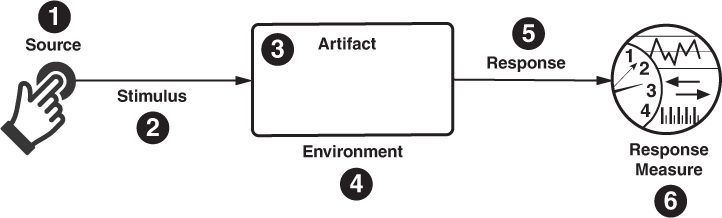
\includegraphics{Figures/qualityattributescenario.jpg}}
\caption{\label{Figure::The parts of a quality attribute scenario} The parts of a quality attribute scenario.}
\end{figure}
\index{Non-functional requirements}\index{testable}\index{unambiguous}\index{Source of stimulus}\index{Stimulus}\index{Environment}\index{Response}\index{Response measure}\index{uptime}\index{error rate}\index{Scenario}
\section{List of Significant Quality Attribute Scenarios\label{Section::SignificantQAS}}
\subsection{Availability\label{subSection::AvailabilityQA}}
\begin{enumerate}
    \item Source of stimulus: A user requests to stitch two images together.
    \item Stimulus: The user clicks on a button to start the stitching process.
    \item Artifact: The two images that the user wants to stitch together.
    \item Environment: The OpenCV Image Stitcher module is running on a computer.
    \item Response: The Image Stitcher module stitches the two images together and displays the result.
    \item Response measure:
    \begin{itemize}
        \item The response measure is the time it takes to stitch the two images together.
        \item The percentage of time that the library is able to process requests and return results without any errors or downtime.
        \item This can be measured using metrics such as uptime, response time, and error rate.
    \end{itemize}
\end{enumerate}
\begin{figure}[H]
\centering
\scalebox{0.6}{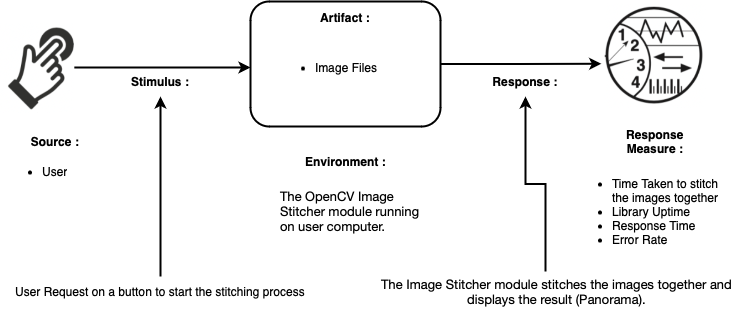
\includegraphics{Figures/Availability.png}}
\caption{\label{Figure::Quality Attribute Scenario for Availability} Quality Attribute Scenario for Availability \cite{drawio}.}
\end{figure}
A high availability score indicates that OpenCV is able to handle a large volume of requests and provide reliable results to users, ensuring that the application is always available and responsive.
In this scenario, the availability quality attribute is met if the Image Stitcher module is able to stitch the two images together in a timely manner. If the Image Stitcher module is not able to stitch the images together, or if it takes a long time to do so, then the availability quality attribute is not met.
\subsection{Deployability\label{subSection::DeployabilityQA}}
\begin{enumerate}
    \item Source of stimulus: A software developer wants to deploy the OpenCV Image Stitcher module in a new application.
    \item Stimulus: The developer downloads the OpenCV Image Stitcher module from the OpenCV website.
    \item Artifact: The OpenCV Image Stitcher module is a C++ library.
    \item Environment: The developer's development environment must have a C++ compiler and the OpenCV libraries installed.
    \item Response: The developer compiles the OpenCV Image Stitcher module and links it to their application.
    \item Response measure: The response measure is the time it takes to deploy the OpenCV Image Stitcher module in the new application.
\end{enumerate} 
\index{Deployability}\index{Energy Efficiency}\index{Integrability}\index{Modifiability}\index{Performance}
\begin{figure}[H]
\centering
\scalebox{0.6}{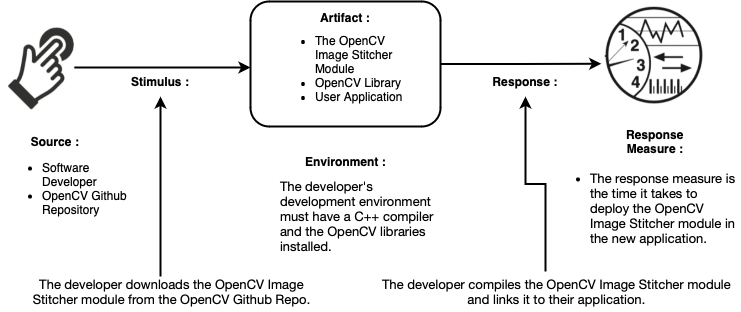
\includegraphics{Figures/Deployability.png}}
\caption{\label{Figure::Quality Attribute Scenario for Deployability} Quality Attribute Scenario for Deployability.}
\end{figure}
In this scenario, the deployability quality attribute is met if the OpenCV Image Stitcher module can be deployed in the new application in a timely manner. If the OpenCV Image Stitcher module cannot be deployed, or if it takes a long time to do so, then the deployability quality attribute is not met.
\subsection{Energy Efficiency\label{subSection::EnergyEfficiencyQA}}
\begin{enumerate}
    \item Source of stimulus: A user wants to use the OpenCV Image Stitcher module to stitch two images together on a mobile device.
    \item Stimulus: The user opens the application that uses the OpenCV Image Stitcher module.
    \item Artifact: The two images that the user wants to stitch together.
    \item Environment: The mobile device has a limited battery life.
    \item Response: The OpenCV Image Stitcher module stitches the two images together and displays the result.
    \item Response measure: The response measure is the amount of energy consumed by the mobile device while the OpenCV Image Stitcher module is running.
\end{enumerate}
\begin{figure}[H]
\centering
\scalebox{0.6}{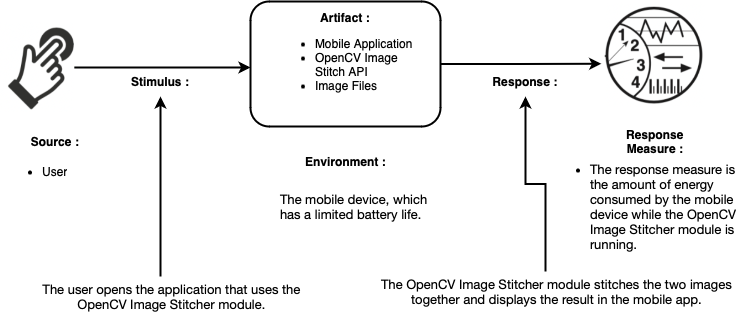
\includegraphics{Figures/energyefficiency.png}}
\caption{\label{Figure::Quality Attribute Scenario for Energy Efficiency} Quality Attribute Scenario for Energy Efficiency.}
\end{figure}
In this scenario, the energy efficiency quality attribute is met if the OpenCV Image Stitcher module is able to stitch the two images together while consuming as little energy as possible. If the OpenCV Image Stitcher module consumes a lot of energy, then the battery life of the mobile device will be reduced.
\subsection{Integrability\label{subSection::IntegrabilityQA}}
\begin{enumerate}
    \item Source of stimulus: Development team
    \item Stimulus: The development team needs to integrate openCV with a new software component.
    \item Artifact: openCV software package, new component
    \item Environment: Development environment with the new software component and its associated hardware and software.
    \item Response: The openCV software package is successfully integrated with the new software component and is fully functional.
    \item Response Measure: The development team measures the time it takes to integrate openCV with the new software component, the number of errors encountered during integration, and the ease of using openCV with the new software component.
\end{enumerate}
\begin{figure}[H]
\centering
\scalebox{0.5}{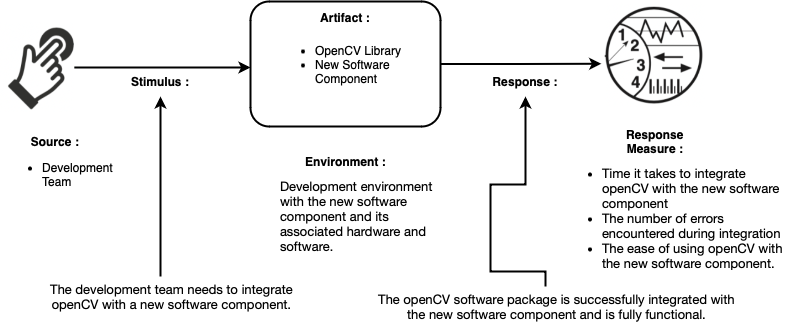
\includegraphics{Figures/Integratability.png}}
\caption{\label{Figure::Quality Attribute Scenario for Integrability} Quality Attribute Scenario for Integrability.}
\end{figure}
Additionally, the team may also measure the impact of the integration on the performance of the new software component and the overall system. The goal is to minimize integration time, errors, and impact on performance, while maximizing ease of use and compatibility with the new software component.
\subsection{Modifiability\label{subSection::ModifiabilityQA}}
\begin{enumerate}
    \item Source of stimulus: Product owner
    \item Stimulus: The product owner requests a new feature to be added to openCV.
    \item Artifact: openCV software package, new feature
    \item Environment: Development environment with the necessary hardware and software.
    \item Response: The development team modifies the openCV software package to include the new feature and ensures that it is fully functional.
    \item Response measure: The development team measures the time it takes to modify openCV to include the new feature, the number of errors encountered during modification, and the impact of the modification on the performance of openCV.
\end{enumerate}
\begin{figure}[H]
\centering
\scalebox{0.5}{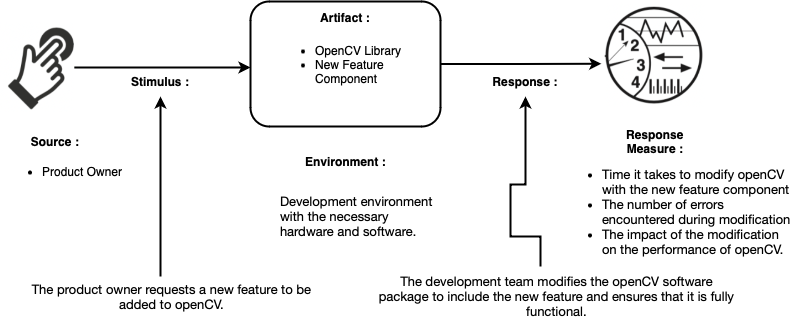
\includegraphics{Figures/modifiability.png}}
\caption{\label{Figure::Quality Attribute Scenario for Modifiability} Quality Attribute Scenario for Modifiability.}
\end{figure}
Additionally, the team may also measure the ease of maintaining the modified code and the impact of the modification on the overall system. The goal is to minimize modification time, errors, and impact on performance, while maximizing ease of maintenance and compatibility with the overall system.
\subsection{Performance\label{subSection::PerformanceQA}}
\begin{enumerate}
    \item Source of stimulus: User
    \item Stimulus: The user requests openCV to process a large image dataset.
    \item Artifact: openCV software package, image dataset, image library
    \item Environment: Production environment with the necessary hardware and software.
    \item Response: openCV processes the large image dataset within an acceptable time frame and with minimal errors.
    \item Response measure: The user measures the time it takes for openCV to process the large image dataset, the number of errors encountered during processing, and the resource utilization of the system during processing.
\end{enumerate}
\begin{figure}[H]
\centering
\scalebox{0.6}{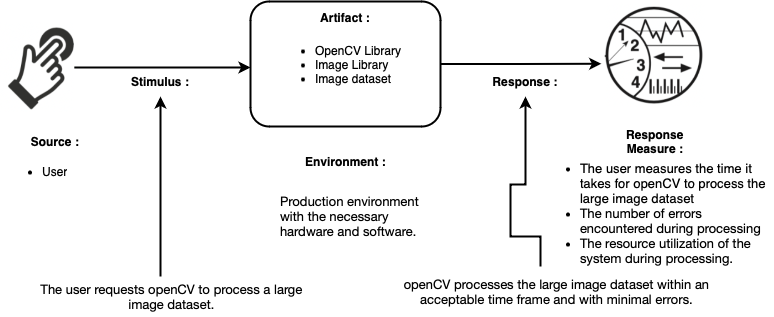
\includegraphics{Figures/Performance.png}}
\caption{\label{Figure::Quality Attribute Scenario for Performance} Quality Attribute Scenario for Performance.}
\end{figure}
Additionally, the user may also measure the accuracy of the processing results and the ease of integrating openCV with other software components in the production environment. The goal is to minimize processing time, errors, and resource utilization, while maximizing accuracy and ease of integration with other software components.
\subsection{Safety\label{subSection::SafetyQA}}
\begin{enumerate}
    \item Source of stimulus: Self-driving car system.
    \item Stimulus: The self-driving car system requests openCV to detect objects on the road and make decisions based on the detected objects.
    \item Artifact: openCV software package, car camera.
    \item Environment: Production environment in a self-driving car with the necessary hardware and software.
    \item Response: openCV accurately detects objects on the road and provides the self-driving car system with the necessary information to make safe driving decisions.
    \item Response measure: The self-driving car system measures the accuracy of openCV's object detection on the road, the number of false positives or false negatives encountered, and the impact of openCV's operation on the safety of the passengers and other vehicles on the road.
\end{enumerate}
\index{Safety}\index{Security}\index{Testability}\index{Usability}
\begin{figure}[H]
\centering
\scalebox{0.6}{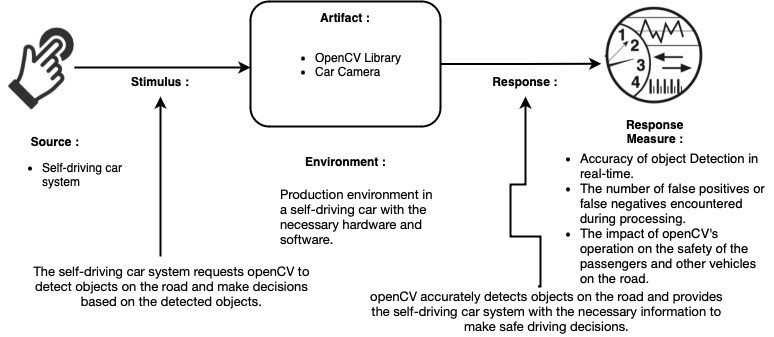
\includegraphics{Figures/Safety.png}}
\caption{\label{Figure::Quality Attribute Scenario for Safety} Quality Attribute Scenario for Safety.}
\end{figure}
Additionally, the system may also measure the ease of integrating openCV with other safety systems in the self-driving car. The goal is to maximize the accuracy of object detection while minimizing any safety hazards or risks associated with openCV's operation in the self-driving car.
\subsection{Security\label{subSection::SecurityQA}}
\begin{enumerate}
    \item Source of stimulus: Unauthorized user
    \item Stimulus: The unauthorized user attempts to gain access to sensitive information or disrupt the operation of openCV.
    \item Artifact: openCV software package, Security log report
    \item Environment: Production environment with the necessary hardware and software.
    \item Response: openCV detects and prevents the unauthorized user's attempts to gain access to sensitive information or disrupt the system's operation and does not compromise the security of the system or any sensitive information.
    \item Response measure: The system measures the number of successful and unsuccessful attempts by the unauthorized user to gain access to sensitive information or disrupt the system's operation, the impact of the unauthorized user's attempts on the security of the system and any sensitive information, and the effectiveness of openCV's security measures in preventing the unauthorized user's attempts.
\end{enumerate}
\begin{figure}[H]
\centering
\scalebox{0.5}{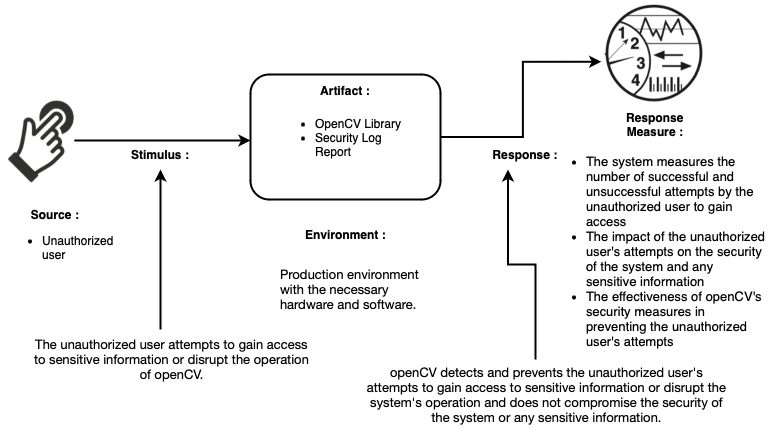
\includegraphics{Figures/Security.png}}
\caption{\label{Figure::Quality Attribute Scenario for Security} Quality Attribute Scenario for Security.}
\end{figure}
Additionally, the system may also measure the ease of maintaining and updating openCV's security measures to address any new vulnerabilities or threats. The goal is to minimize the number of successful unauthorized access attempts and their impact on the security of the system and any sensitive information.
\subsection{Testability\label{subSection::TestabilityQA}}
\begin{enumerate}
    \item Source of stimulus: Testing team
    \item Stimulus: The testing team needs to test the accuracy and performance of the openCV Image Stitching module in a real-world scenario.
    \item Artifact: openCV Image Stitching module, Image files
    \item Environment: Real-world environment with the necessary hardware and software on tester's computer.
    \item Response: The openCV Image Stitching module accurately stitches images in the real-world scenario and performs within acceptable performance parameters.
    \item Response measure: The testing team measures the accuracy of the openCV Image Stitching module in stitching images in the real-world scenario, the number of errors encountered during stitching, and the performance of the module in terms of processing time and resource utilization. Test-cases pass percentage for unique scenarios. Test Coverage percentage of openCV Image Stitching module.
\end{enumerate}
\begin{figure}[H]
\centering
\scalebox{0.5}{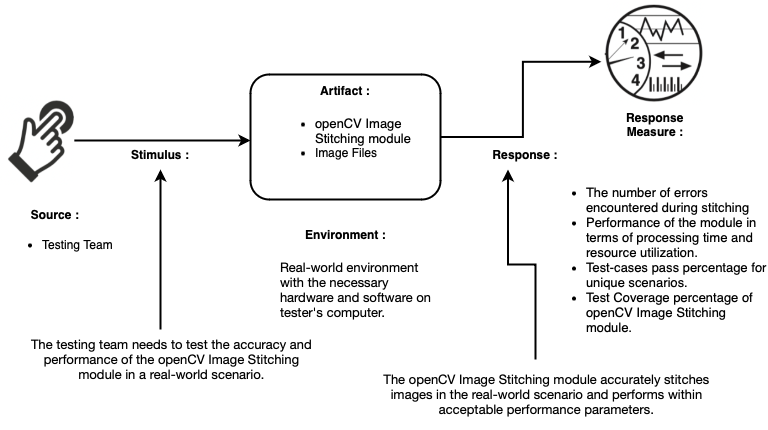
\includegraphics{Figures/Testability.png}}
\caption{\label{Figure::Quality Attribute Scenario for Testability} Quality Attribute Scenario for Testability.}
\end{figure}
Additionally, the team may also measure the ease of testing the openCV Image Stitching module in the real-world scenario and the effectiveness of any testing tools or frameworks used. The goal is to maximize the accuracy and performance of the openCV Image Stitching module in the real-world scenario while minimizing any testing time and effort required.
\subsection{Usability\label{subSection::UsabilityQA}}
\begin{enumerate}
    \item Source of stimulus: User
    \item Stimulus: The user needs to use openCV to perform image processing tasks.
    \item Artifact: openCV software package, image files
    \item Environment: User's environment with the necessary hardware and software.
    \item Response: The user is able to use openCV to perform image processing tasks with ease and efficiency.
    \item Response measure: The user measures the ease of learning and using openCV to perform image processing tasks, the time it takes to complete the tasks, and the user satisfaction with the user interface and overall usability of openCV.
\end{enumerate}
\begin{figure}[H]
\scalebox{0.5}{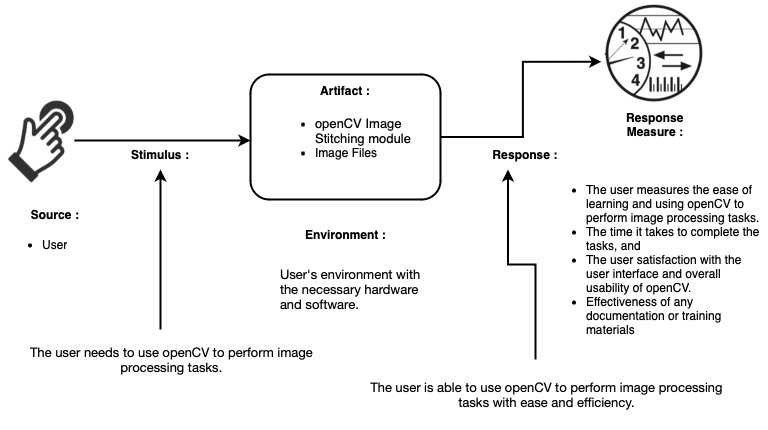
\includegraphics{Figures/Usability.png}}
\caption{\label{Figure::Quality Attribute Scenario for Usability} Quality Attribute Scenario for Usability.}
\end{figure}
Additionally, the user may also measure the effectiveness of any documentation or training materials provided with openCV. The goal is to maximize the ease of use and efficiency of openCV for image processing tasks, while minimizing the time and effort required to learn and use the software.
\section{Evaluation of Business risk and Architectural Significance\label{Section::QAratings}}
\begin{longtable}{|l|c|c|}
\hline
\textbf{Quality Attribute} & \textbf{Business Value (a)} & \textbf{Effect on Architecture (b)} \\
\hline
Availability & H & M \\
Deployability & M & M \\
Energy Efficiency & L & M \\
Integrability & M & M \\
Modifiability & H & M \\
Performance & H & H \\
Safety & H & H \\
Security & H & H \\
Testability & H & M \\
Usability & M & M \\
\hline
\caption{Quality Attribute Evaluation \label{Table::Quality Attribute Evaluation}}
\end{longtable}
\newpage
\subsection{Understanding the values}
Grading Scale Used:\newline
\newline
\underline{\textbf{Rating:}} (a, b):\newline
\textbf{a:} the ASR’s\index{ASR!Architecturally significant requirement} business value\index{Business Value}(importance)\newline
\textbf{b:} the effect on the architecture(difficulty)\newline
\\
\underline{\textbf{Key:}}\newline
\textbf{H}=high\newline
\textbf{M}=medium\newline
\textbf{L}=low\newline
\begin{enumerate}
    \item Availability: openCV is a mature library with a large community of users and developers. There are many different ways to install and use openCV, which makes it easy to deploy in a variety of environments. This is why we rated availability as high.
    \item Deployability: openCV is available for a variety of platforms, including Windows, Linux, and macOS. There are also many different ways to deploy openCV, such as as a static library, a shared library, or a Docker image. This is why we rated deployability as medium.
    \item Energy Efficiency: openCV uses a variety of techniques to optimize its performance, such as using hardware acceleration and image compression. This is why we rated energy efficiency as low.
    \item Integrability: openCV provides a variety of APIs, such as C++, Python, and Java, which make it easy to integrate with other languages and frameworks. This is why we rated integrabilty as medium.
    \item Modifiability: openCV is a open source library, which means that the source code is available for anyone to modify. This makes it easy to customize openCV to meet the specific needs of a project. This is why we rated modifiability as high.
    \item Performance: openCV is designed to be fast and efficient, even on resource-constrained devices. This is why we rated performance as high.
    \item Safety: openCV is designed to be secure and reliable, even in critical applications. This is why I rated safety as high.
    \item Security: openCV is designed to be resistant to attack and intrusion. This is why we rated security as high.
    \item Testability: openCV provides a variety of tools and resources to help developers test their code. This makes it easy to ensure that openCV is working properly before it is deployed in production. This is why we rated testability as high.
    \item Usability: openCV provides a variety of documentation and tutorials to help developers get started. This makes it easy for anyone to use openCV, regardless of their experience level. This is why we rated usability as medium.
\end{enumerate}
\section{Utiltity Tree\label{Section::utilityTree}}
\subsection{Introduction}
\paragraph{} A utility tree starts with the root node "Utility" representing the overall "goodness" of the system. Major Quality Attributes (QAs) are listed under the root node. Each QA is then further refined with specific aspects relevant to the system. These refinements can be broken down into specific Quality Attribute Scenarios (ASRs).
\paragraph{} ASRs are placed as leaves on the tree and evaluated based on business value and technical risk. Business value is assessed as high, medium, or low, indicating the importance of meeting the requirement. Technical risk is evaluated as high, medium, or low, reflecting the level of concern and confidence in meeting the ASR.
\paragraph{} In summary, a utility tree outlines the system's QAs, their refinements, and ASRs as scenarios. These scenarios are then evaluated based on business value and technical risk.
\subsection{Tabular form of Utility Tree}
\begin{figure}[H]
\centering
\scalebox{0.55}{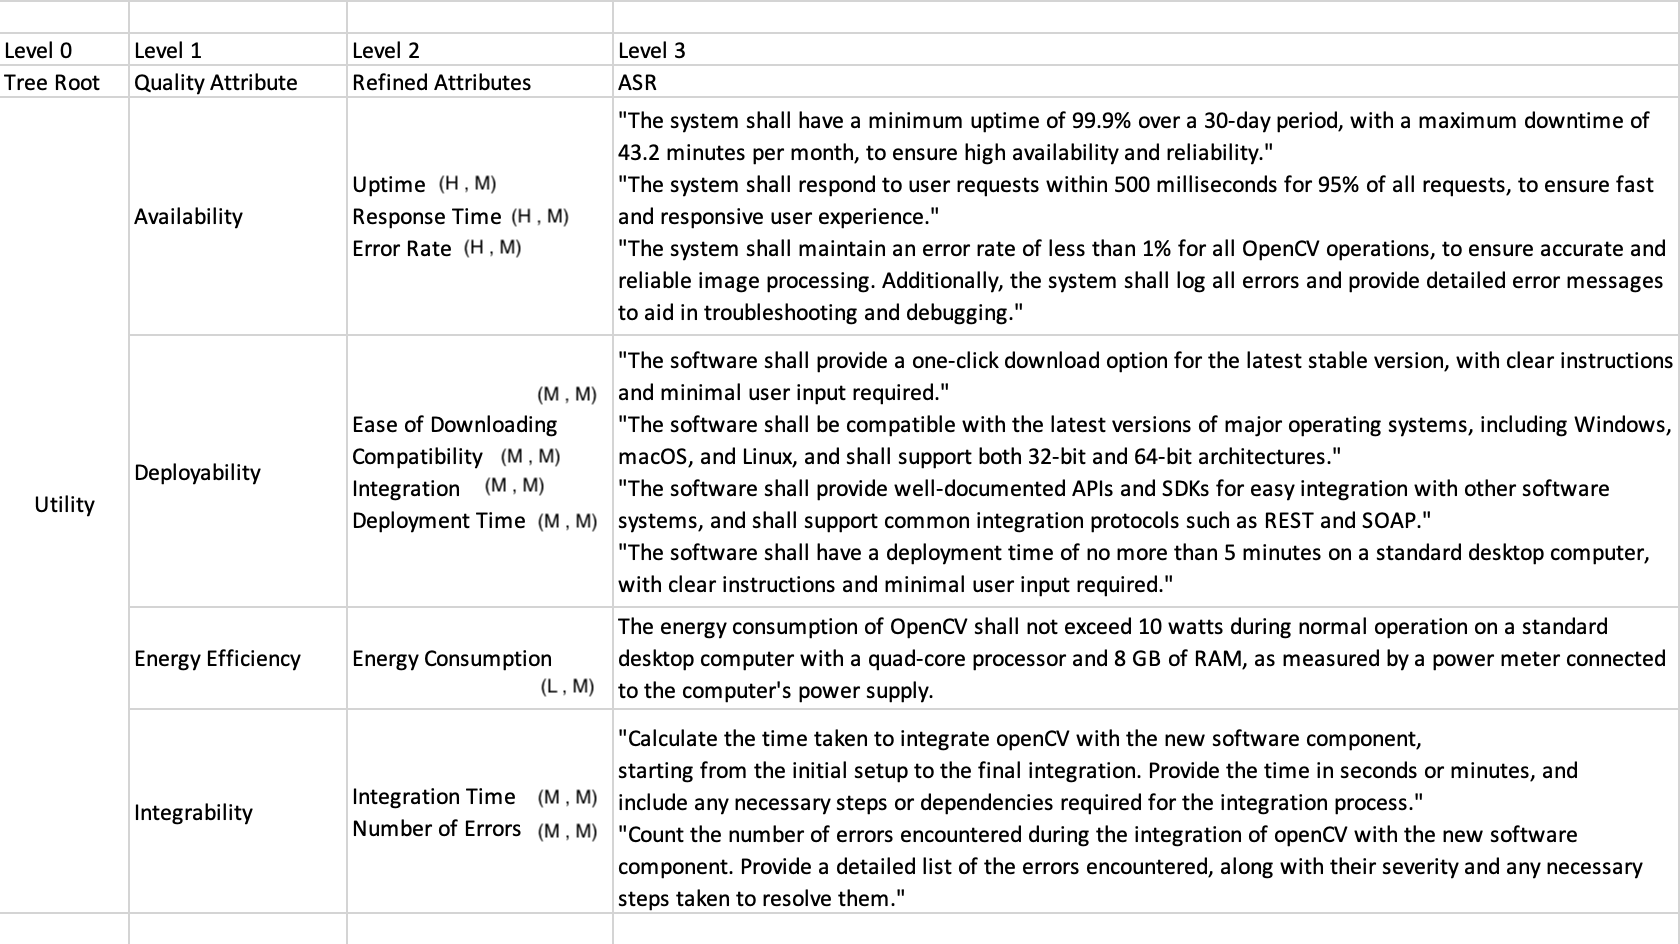
\includegraphics{Figures/UtilityTree1.png}}
\caption{\label{Figure::UtilityTree1} Utility Tree - 1.}
\end{figure}
\begin{figure}[H]
\centering
\scalebox{0.5}{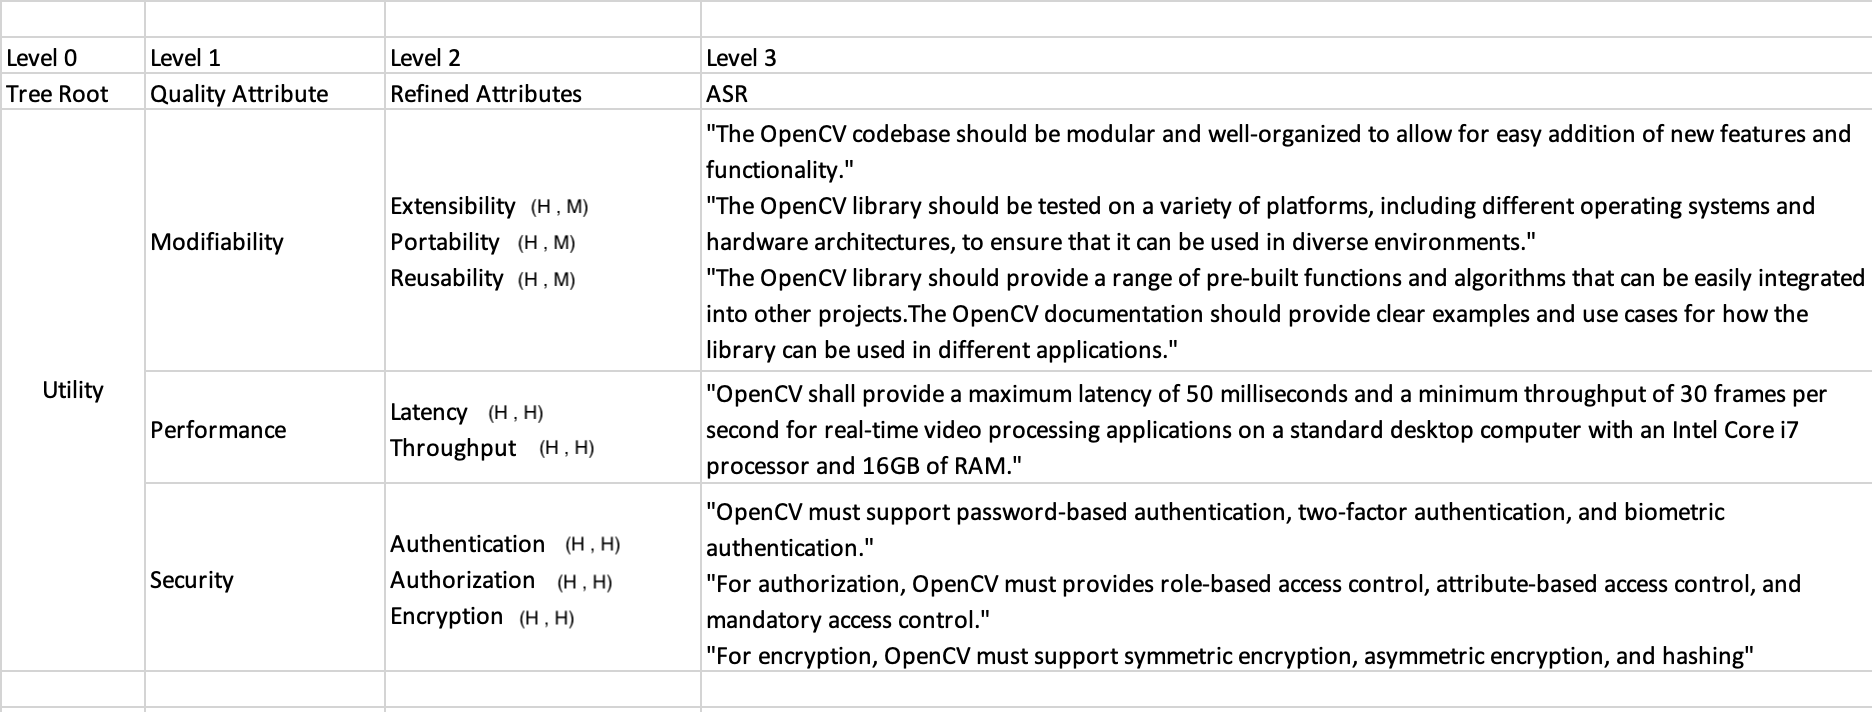
\includegraphics{Figures/UtilityTree2.png}}
\caption{\label{Figure::UtilityTree2} Utility Tree - 2.}
\end{figure}
\begin{figure}[H]
\centering
\scalebox{0.5}{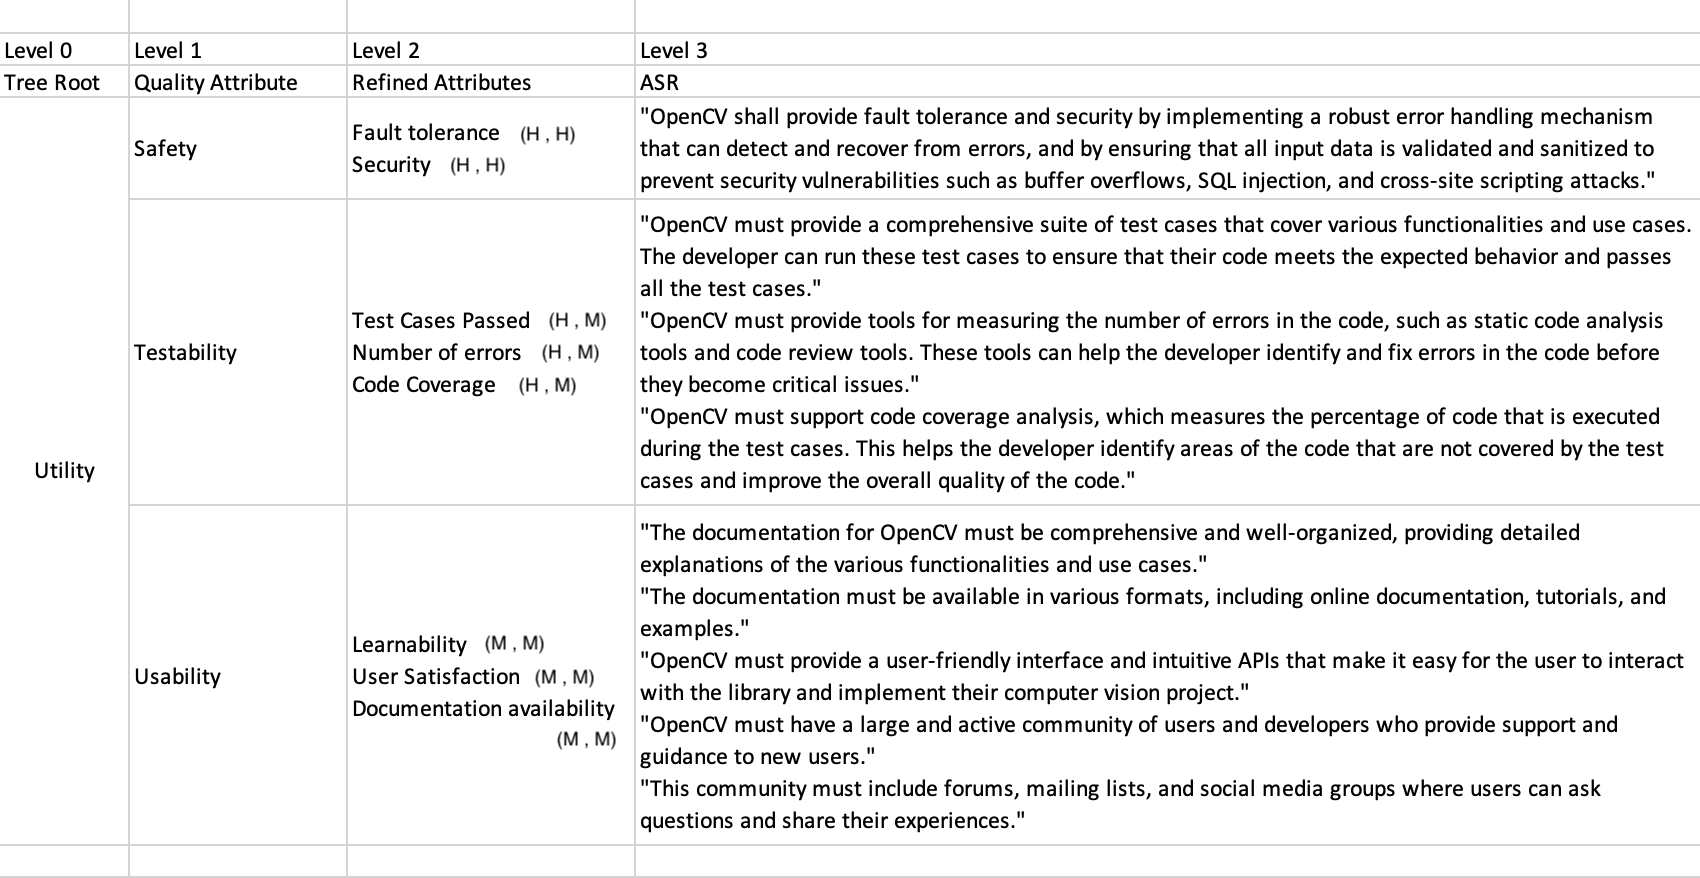
\includegraphics{Figures/UtilityTree3.png}}
\caption{\label{Figure::UtilityTree3} Utility Tree - 3.}
\end{figure}
\chapter{Risks\\
\small{\textit{-- Nikhil Kumar G, Raj Palival}}
\index{Chapter!Risks}
\index{Risks}
\label{Chapter::Risks}}

\section{Introduction \label{Section::RisksChapterIntro}}
OpenCV, like any software, is not immune to risks and challenges. While it is a powerful and widely-used open-source computer vision library, it's important to recognize that there may be potential pitfalls that can impact its usage and effectiveness. These risks can manifest in various areas, such as functionality, performance, security, compatibility, and documentation. Understanding these risks allows developers to be proactive in addressing them and ensuring the smooth integration and deployment of OpenCV in their applications. By staying informed, keeping up with updates, seeking community support, and following best practices, developers can mitigate these risks and harness the full potential of OpenCV for their computer vision needs.

\section{Risks \label{Section::Risks}}
Based on observations and investigations, there are a few anticipated risks and areas that can be improved in OpenCV:

\subsection{Security Risks \label{subSection::SecurityRisk}}
\begin{enumerate}
     \item OpenCV may be vulnerable to security attacks such as buffer overflows or injection attacks, which can lead to unauthorized access or control of systems.
     \item Malicious users could exploit vulnerabilities in the library, potentially causing damage or compromising sensitive data.     
 \end{enumerate}

\subsubsection{Tactics for Security Risks \label{subsubSection::SecurityTactic}}
The tactics that can be applied to above risks are:
\begin{itemize}
    \item Regularly update OpenCV to the latest version to incorporate security patches and fixes.
    \item Implement secure coding practices when using OpenCV, such as input validation and proper memory management.
    \item Perform security audits and vulnerability assessments to identify and mitigate potential risks.
    \item Encourage the OpenCV community to report and address security issues promptly.
\end{itemize}
\index{pitfalls}\index{manifest}\index{Security Risks}\index{Tactics}\index{memory management}
\subsection{Performance Risks \label{subSection::PerformanceRisk}}
\begin{enumerate}
     \item OpenCV may face performance limitations, especially when processing large-scale or real-time video streams or when working with resource-intensive algorithms.
     \item Inefficient use of system resources or suboptimal algorithms could result in slow execution or inadequate responsiveness.    
 \end{enumerate}

 \subsubsection{Tactics for Performance Risks \label{subsubSection::PerformanceTactic}}
The tactics that can be applied to above risks are:
\begin{itemize}
    \item Optimize algorithms and data structures to enhance computational efficiency.
    \item Leverage hardware acceleration technologies like GPU (Graphics Processing Unit) or dedicated AI accelerators when applicable.
    \item Employ parallel processing techniques, such as multi-threading or distributed computing, to distribute computational load and improve performance.
    \item Continuously benchmark and profile OpenCV applications to identify bottlenecks and areas for optimization.
\end{itemize}

\subsection{Usability Risks \label{subSection::UsabilityRisk}}
\begin{enumerate}
     \item OpenCV has a steep learning curve for newcomers and may be challenging for developers without a strong background in computer vision.
     \item Documentation may be insufficient or not beginner-friendly, making it difficult to understand and utilize the library effectively.   
 \end{enumerate}

 \subsubsection{Tactics for Usability Risks \label{subsubSection::UsabilityTactic}}
The tactics that can be applied to above risks are:
\begin{itemize}
    \item Enhance the official OpenCV documentation with comprehensive and well-structured tutorials, examples, and explanations.
    \item Foster an active community that provides support, answers questions, and shares best practices.
    \item Develop user-friendly APIs and higher-level abstractions to simplify common computer vision tasks.
    \item Provide educational resources, such as online courses or workshops, to help developers acquire the necessary skills to use OpenCV effectively.
\end{itemize}
\index{Performance Risks}\index{suboptimal algorithms}\index{resource-intensive algorithms}\index{Usability Risks}\index{computational load} \index{multi-threading} \index{distributed computing}
\subsection{Compatibility and Portability Risks \label{subSection::CompatibilityRisk}}
\begin{enumerate}
     \item OpenCV may face compatibility issues with different operating systems, hardware architectures, or versions of dependencies.
     \item Lack of portability can limit the usage of OpenCV in diverse environments or on specific platforms.  
 \end{enumerate}

 \subsubsection{Tactics for Compatibility and Portability Risks \label{subsubSection::CompatibilityTactic}}
The tactics that can be applied to above risks are:
\begin{itemize}
     \item Conduct extensive testing on different platforms and environments to identify and resolve compatibility issues.
     \item Follow best practices for cross-platform development and ensure proper handling of platform-specific features or dependencies.
     \item Provide pre-compiled binaries or packages for popular operating systems to simplify installation and deployment.
     \item Encourage community contributions and feedback to address compatibility issues specific to certain environments.
\end{itemize}

\subsection{Documentation Risks \label{subSection::DocumentationRisk}}
\begin{enumerate}
     \item OpenCV's documentation may lack clarity, completeness, or up-to-date information, leading to confusion and difficulties for developers.
     \item Inadequate learning resources can make it challenging for beginners to grasp the concepts and effectively utilize the library. 
 \end{enumerate}

 \subsubsection{Tactics for Documentation Risks \label{subsubSection::DocumentationTactic}}
The tactics that can be applied to above risks are:
\begin{itemize}
     \item Establish clear and well-structured documentation that covers all aspects of OpenCV, including detailed explanations, API references, and usage examples.
     \item Maintain an active and accessible community forum or support channel to address questions and provide guidance.
     \item Collaborate with educational institutions or organizations to develop comprehensive learning resources, tutorials, and courses for OpenCV.
     \item Encourage community contributions to enhance documentation and create additional learning materials.
\end{itemize}
\index{Portability Risks}\index{Documentation Risks}\index{Accuracy}\index{Robustness Risks}\index{datasets}
\subsection{Accuracy and Robustness Risks \label{subSection::RobustnessRisk}}
\begin{enumerate}
     \item OpenCV's computer vision algorithms may exhibit inaccuracies or lack robustness in certain scenarios or edge cases.
     \item Performance degradation or incorrect results can occur when the algorithms fail to handle specific image variations or conditions. 
 \end{enumerate}

 \subsubsection{Tactics for Accuracy and Robustness Risks \label{subsubSection::RobustnessTactic}}
The tactics that can be applied to above risks are:
\begin{itemize}
     \item Continuously evaluate and benchmark the performance and accuracy of OpenCV algorithms across a wide range of test cases and datasets.
     \item Collect and analyze user feedback and reported issues to identify areas where algorithms need improvement.
     \item Encourage collaboration and contributions from the computer vision research community to refine and enhance existing algorithms.
     \item Maintain a well-organized repository of sample images and datasets to facilitate testing and evaluation of algorithmic performance.
\end{itemize}
\index{Scalability}\index{Concurrency Risks}\index{Intel TBB}\index{OpenMP}\index{Privacy Risk}
\subsection{Scalability and Concurrency Risks \label{subSection::ScalabilityRisk}}
\begin{enumerate}
     \item OpenCV may encounter challenges in scaling and efficiently utilizing multiple processing cores or distributed computing resources.
     \item In scenarios where high concurrency is required, such as real-time video processing or large-scale computer vision pipelines, performance bottlenecks or resource contention can arise.
 \end{enumerate}

 \subsubsection{Tactics for Scalability and Concurrency Risks \label{subsubSection::ScalabilityTactic}}
The tactics that can be applied to above risks are:
\begin{itemize}
     \item Implement parallel processing techniques, such as multi-threading or task-based concurrency, to distribute workloads and maximize resource utilization.
     \item Utilize frameworks or libraries that offer higher-level concurrency abstractions, such as OpenMP or Intel TBB, to simplify parallel programming in OpenCV.
     \item Optimize critical sections of code and minimize thread synchronization overhead to improve scalability and reduce contention.
     \item Explore distributed computing frameworks, such as Apache Spark or Hadoop, for processing large-scale computer vision tasks across multiple machines.
\end{itemize}

\subsection{Data Privacy Risks \label{subSection::PrivacyRisk}}
\begin{enumerate}
     \item OpenCV applications may process and analyze sensitive data, such as images containing personally identifiable information or proprietary content.
     \item Inadequate data privacy measures can lead to privacy breaches or unauthorized access to confidential information.
 \end{enumerate}

 \subsubsection{Tactics for Data Privacy Risks \label{subsubSection::PrivacyTactic}}
The tactics that can be applied to above risks are:
\begin{itemize}
     \item Adhere to relevant data privacy regulations and standards, such as GDPR or HIPAA, when handling sensitive data with OpenCV.
     \item Implement data anonymization techniques to remove or obfuscate personally identifiable information from images or other data inputs.
     \item Employ encryption mechanisms to protect data at rest or in transit during OpenCV processing.
     \item Educate developers on best practices for data privacy and encourage the use of secure coding principles when working with OpenCV.
\end{itemize}

\subsection{Community Engagement Risks \label{subSection::CommunityRisk}}
\begin{enumerate}
     \item OpenCV may face challenges in actively engaging the community and effectively incorporating user feedback and contributions.
     \item Limited community involvement can result in slower resolution of issues, missed opportunities for improvement, and reduced adoption.
 \end{enumerate}

 \subsubsection{Tactics for Community Engagement Risks \label{subsubSection::CommunityTactic}}
The tactics that can be applied to above risks are:
\begin{itemize}
     \item Foster an inclusive and collaborative community environment where users feel encouraged to provide feedback, report issues, and contribute to the development of OpenCV.
     \item Establish transparent communication channels, such as mailing lists, forums, or dedicated feedback platforms, to gather and address user input effectively.
     \item Regularly acknowledge and appreciate community contributions through recognition, documentation credits, or code attribution.
     \item Actively participate in computer vision conferences, workshops, and hackathons to engage with the broader community and promote OpenCV's advancements.
\end{itemize}

\subsection{Integration Risks \label{subSection::IntegrationRisk}}
\begin{enumerate}
     \item OpenCV's integration with machine learning frameworks and libraries may face challenges in terms of compatibility, ease of use, or performance.
     \item Inadequate integration can hinder the adoption of state-of-the-art machine learning techniques within OpenCV applications.
 \end{enumerate}
\index{Integration Risks}
 \subsubsection{Tactics for Integration Risks \label{subsubSection::IntegrationTactic}}
The tactics that can be applied to above risks are:
\begin{itemize}
     \item Establish seamless integration with popular machine learning frameworks, such as TensorFlow or PyTorch, by providing dedicated APIs or interoperability layers.
     \item Offer pre-trained models or model conversion tools that enable users to easily leverage deep learning models within OpenCV.
     \item Collaborate with the machine learning community to identify and address integration issues, ensure compatibility, and keep up with the latest advancements in the field.
     \item Provide extensive documentation and examples showcasing the integration of OpenCV with machine learning, covering common use cases and best practices.
\end{itemize}


\chapter{Architecture\\
\small{\textit{-- Nikhil Kumar G, Raj Palival}}
\index{Chapter!Architecture}
\index{Architecture}
\label{Chapter::Architecture}}

\section{Description\label{Section::ArchitectureIntro}}
OpenCV (Open Source Computer Vision Library \cite{OCV}) is an open-source library that includes several hundreds of computer vision algorithms. It has a modular structure architecture, which means that the package includes several modules with shared or static libraries. 

\section{Modules \label{subSection::ModulesList}}
There are two types of modules available:
\begin{enumerate}
     \item Main Modules: These modules are the core components of the OpenCV library that provide essential computer vision functionalities.
     \item Extra modules: These are additional modules that offer extended features and algorithms not included in the main modules.
 \end{enumerate}
Below is a list of all the modules available in each category:

\subsection{Main Modules\label{subSection::MainModules}}
\begin{enumerate}
     \item core. Core functionality: a compact module defining basic data structures, including the dense multi-dimensional array Mat and basic functions used by all other modules. \index{Core functionality}
     \item imgproc. Image Processing: an image processing module that includes linear and non-linear image filtering, geometrical image transformations (resize, affine and perspective warping, generic table-based remapping), color space conversion, histograms, and so on. \index{Image Processing}
     \item imgcodecs. Image file reading and writing: This module in OpenCV provides functions for reading and writing image files in various formats \index{imgcodecs}
     \item videoio. Video I/O: This module in OpenCV provides functions for reading and writing video files and accessing video streams from cameras or other devices. \index{videoio}
     \item highgui. High-level GUI: This module in OpenCV provides high-level functions for creating graphical user interfaces (GUI) to display and interact with images, videos, and other visual data. \index{High-level GUI}
     \item video. Video Analysis: This module in OpenCV involves performing various operations on video frames, such as object detection, tracking, motion analysis, and frame manipulation. \index{object detection}
     \item calib3d. Camera Calibration and 3D Reconstruction: This module in OpenCV provides functions for camera calibration and 3D reconstruction. \index{Camera Calibration}
     \item features2d. 2D Features Framework: This module in OpenCV provides a framework for detecting and describing 2D image features. These features can be used for tasks such as image matching, object recognition, and image stitching. \index{2D Features Framework}
     \item objdetect. Object Detection: This module in OpenCV provides functions and pre-trained models for object detection. It allows you to detect and localize objects within images or video frames.\index{objdetect}
     \item dnn. Deep Neural Network module: This module in OpenCV provides a flexible and efficient framework for working with deep neural networks (DNNs). It allows you to load pre-trained models, perform inference on images or videos, and fine-tune models. \index{Deep Neural Network}
     \item ml. Machine Learning: This module in OpenCV provides a set of machine learning algorithms and tools for various tasks, including classification, regression, clustering, and dimensionality reduction.\index{Machine Learning}
     \item flann. Clustering and Search in Multi-Dimensional Spaces: This module in OpenCV provides efficient algorithms for clustering and searching in multi-dimensional spaces. FLANN stands for Fast Library for Approximate Nearest Neighbors. \index{Clustering}
     \item photo. Computational Photography: This module refers to the use of computational techniques and algorithms to enhance or modify digital photographs.\index{Computational Photography} 
     \item stitching. Images stitching: Image stitching is the process of combining multiple overlapping images to create a larger, seamless panorama. \index{Images stitching}
     \item gapi. Graph API: This module is a computational graph-based framework provided by OpenCV that allows for efficient parallel execution of image processing and computer vision algorithms. \index{Graph API}
 \end{enumerate}
 \subsection{Extra Modules\label{subSection::ExtraModules}}
\begin{enumerate}
     \item alphamat. Alpha Matting \index{Alpha Matting}
     \item aruco. Aruco markers, module functionality was moved to objdetect module \index{Aruco markers}
     \item barcode. Barcode detecting and decoding methods \index{Barcode detecting}
     \item bgsegm. Improved Background-Foreground Segmentation Methods \index{Segmentation}
     \item bioinspired. Biologically inspired vision models and derivated tools \index{bioinspired}
     \item ccalib. Custom Calibration Pattern for 3D reconstruction
     \item cudaarithm. Operations on Matrices
     \item cudabgsegm. Background Segmentation
     \item cudacodec. Video Encoding/Decoding
     \item cudafeatures2d. Feature Detection and Description
     \item cudafilters. Image Filtering
     \item cudaimgproc. Image Processing
     \item cudalegacy. Legacy support
     \item cudaobjdetect. Object Detection
     \item cudaoptflow. Optical Flow
     \item cudastereo. Stereo Correspondence
     \item cudawarping. Image Warping
     \item cudev. Device layer
     \item cvv. GUI for Interactive Visual Debugging of Computer Vision Programs
     \item datasets. Framework for working with different datasets
     \item dnn objdetect. DNN used for object detection
     \item dnn superres. DNN used for super resolution
     \item dpm. Deformable Part-based Models
     \item face. Face Analysis
     \item freetype. Drawing UTF-8 strings with freetype/harfbuzz
     \item fuzzy. Image processing based on fuzzy mathematics
     \item hdf. Hierarchical Data Format I/O routines
     \item hfs. Hierarchical Feature Selection for Efficient Image Segmentation
     \item img hash. The module brings implementations of different image hashing algorithms.
     \item intensity transform. The module brings implementations of intensity transformation algorithms to adjust image contrast.
     \item julia. Julia bindings for OpenCV
     \item line descriptor. Binary descriptors for lines extracted from an image
     \item mcc. Macbeth Chart module
     \item optflow. Optical Flow Algorithms
     \item ovis. OGRE 3D Visualiser
     \item phase unwrapping. Phase Unwrapping API
     \item plot. Plot function for Mat data
     \item quality. Image Quality Analysis (IQA) API
     \item rapid. silhouette based 3D object tracking
     \item reg. Image Registration
     \item rgbd. RGB-Depth Processing
     \item saliency. Saliency API
     \item sfm. Structure From Motion
     \item shape. Shape Distance and Matching
     \item stereo. Stereo Correspondance Algorithms
     \item structured light. Structured Light API
     \item superres. Super Resolution
     \item surface matching. Surface Matching
     \item text. Scene Text Detection and Recognition
     \item tracking. Tracking API
     \item videostab. Video Stabilization
     \item viz. 3D Visualizer
     \item wechat qrcode. WeChat QR code detector for detecting and parsing QR code.
     \item xfeatures2d. Extra 2D Features Framework
     \item ximgproc. Extended Image Processing
     \item xobjdetect. Extended object detection
     \item xphoto. Additional photo processing algorithms
\end{enumerate}

\section{Grouping Modules\label{Section::GroupingModules}}
The modules don't have a clear order or hierarchy. Core, python, and java are commonly used modules, but there isn't a definite separation between them. Often, a module that uses the core module also depends on another module, which makes the structure very complex.\\\\
However, we can group all the modules in three categories:
\begin{enumerate}
     \item Main Functionality
     \item Extended Functionality
     \item High Level GUI
\end{enumerate}

\section{15 Most Important Modules\label{Section::HighLevelView}}
Below is a figure of the 15 most important modules in the three categories discussed above:
\begin{figure}[H]
     \centering
     \scalebox{0.8}{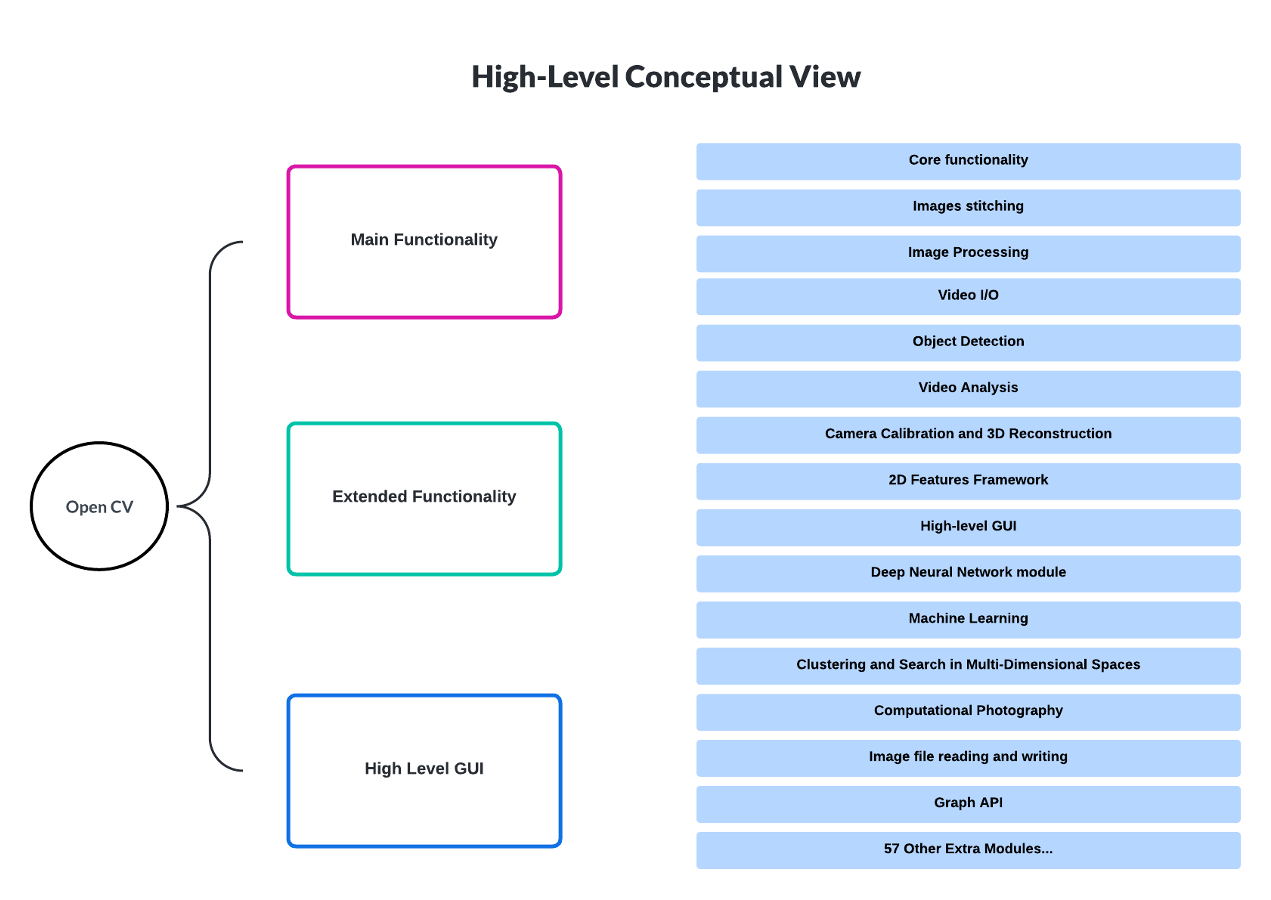
\includegraphics{Figures/Conceptualview.png}}
     \caption{\label{Figure::HighLevelView} High Level Conceptual View}
\end{figure}
\pagebreak

\section{4+1 View of Architecture\label{Section::4+1view}}
The 4+1 architectural view model provides multiple perspectives on the architecture of a system \cite{UNB}. Such as:
\begin{enumerate}
         \item Implementation View
         \item Use Case View
         \item Logical View
         \item Process View
         \item Deployment View
\end{enumerate}
We will use an example of one module to explain the rest of the OpenCV modules in OpenCV’s architecture. More on this later.
\subsection{Implementation View\label{subSection::ImplementationView}} \index{Implementation View}
The implementation view is an architectural view that  provides a detailed perspective on how the system is implemented and how the implementation artifacts are organized and interact with each other.\\\\
     In our case we will consider the following:
     \begin{itemize}
         \item Perspective: Developers, Proj. mngs.
         \item Stage: Design
         \item Focus: Subsystem decomposition
         \item Concerns: Software management
         \item Artefacts: Modules structure, Package diagram
     \end{itemize}
\subsubsection{Implementation View Artefacts\label{subsubSection::ImplementationView}} \index{Artefacts}
The modules structure below shows how all the modules in OpenCV interact with each other. It is clear that the modules in OpenCV are interconnected in a very complex way. \\\\

Modules Structure: Diagram taken from source \cite{OGB} 

\begin{figure}[H]
     \centering
     \scalebox{0.15}{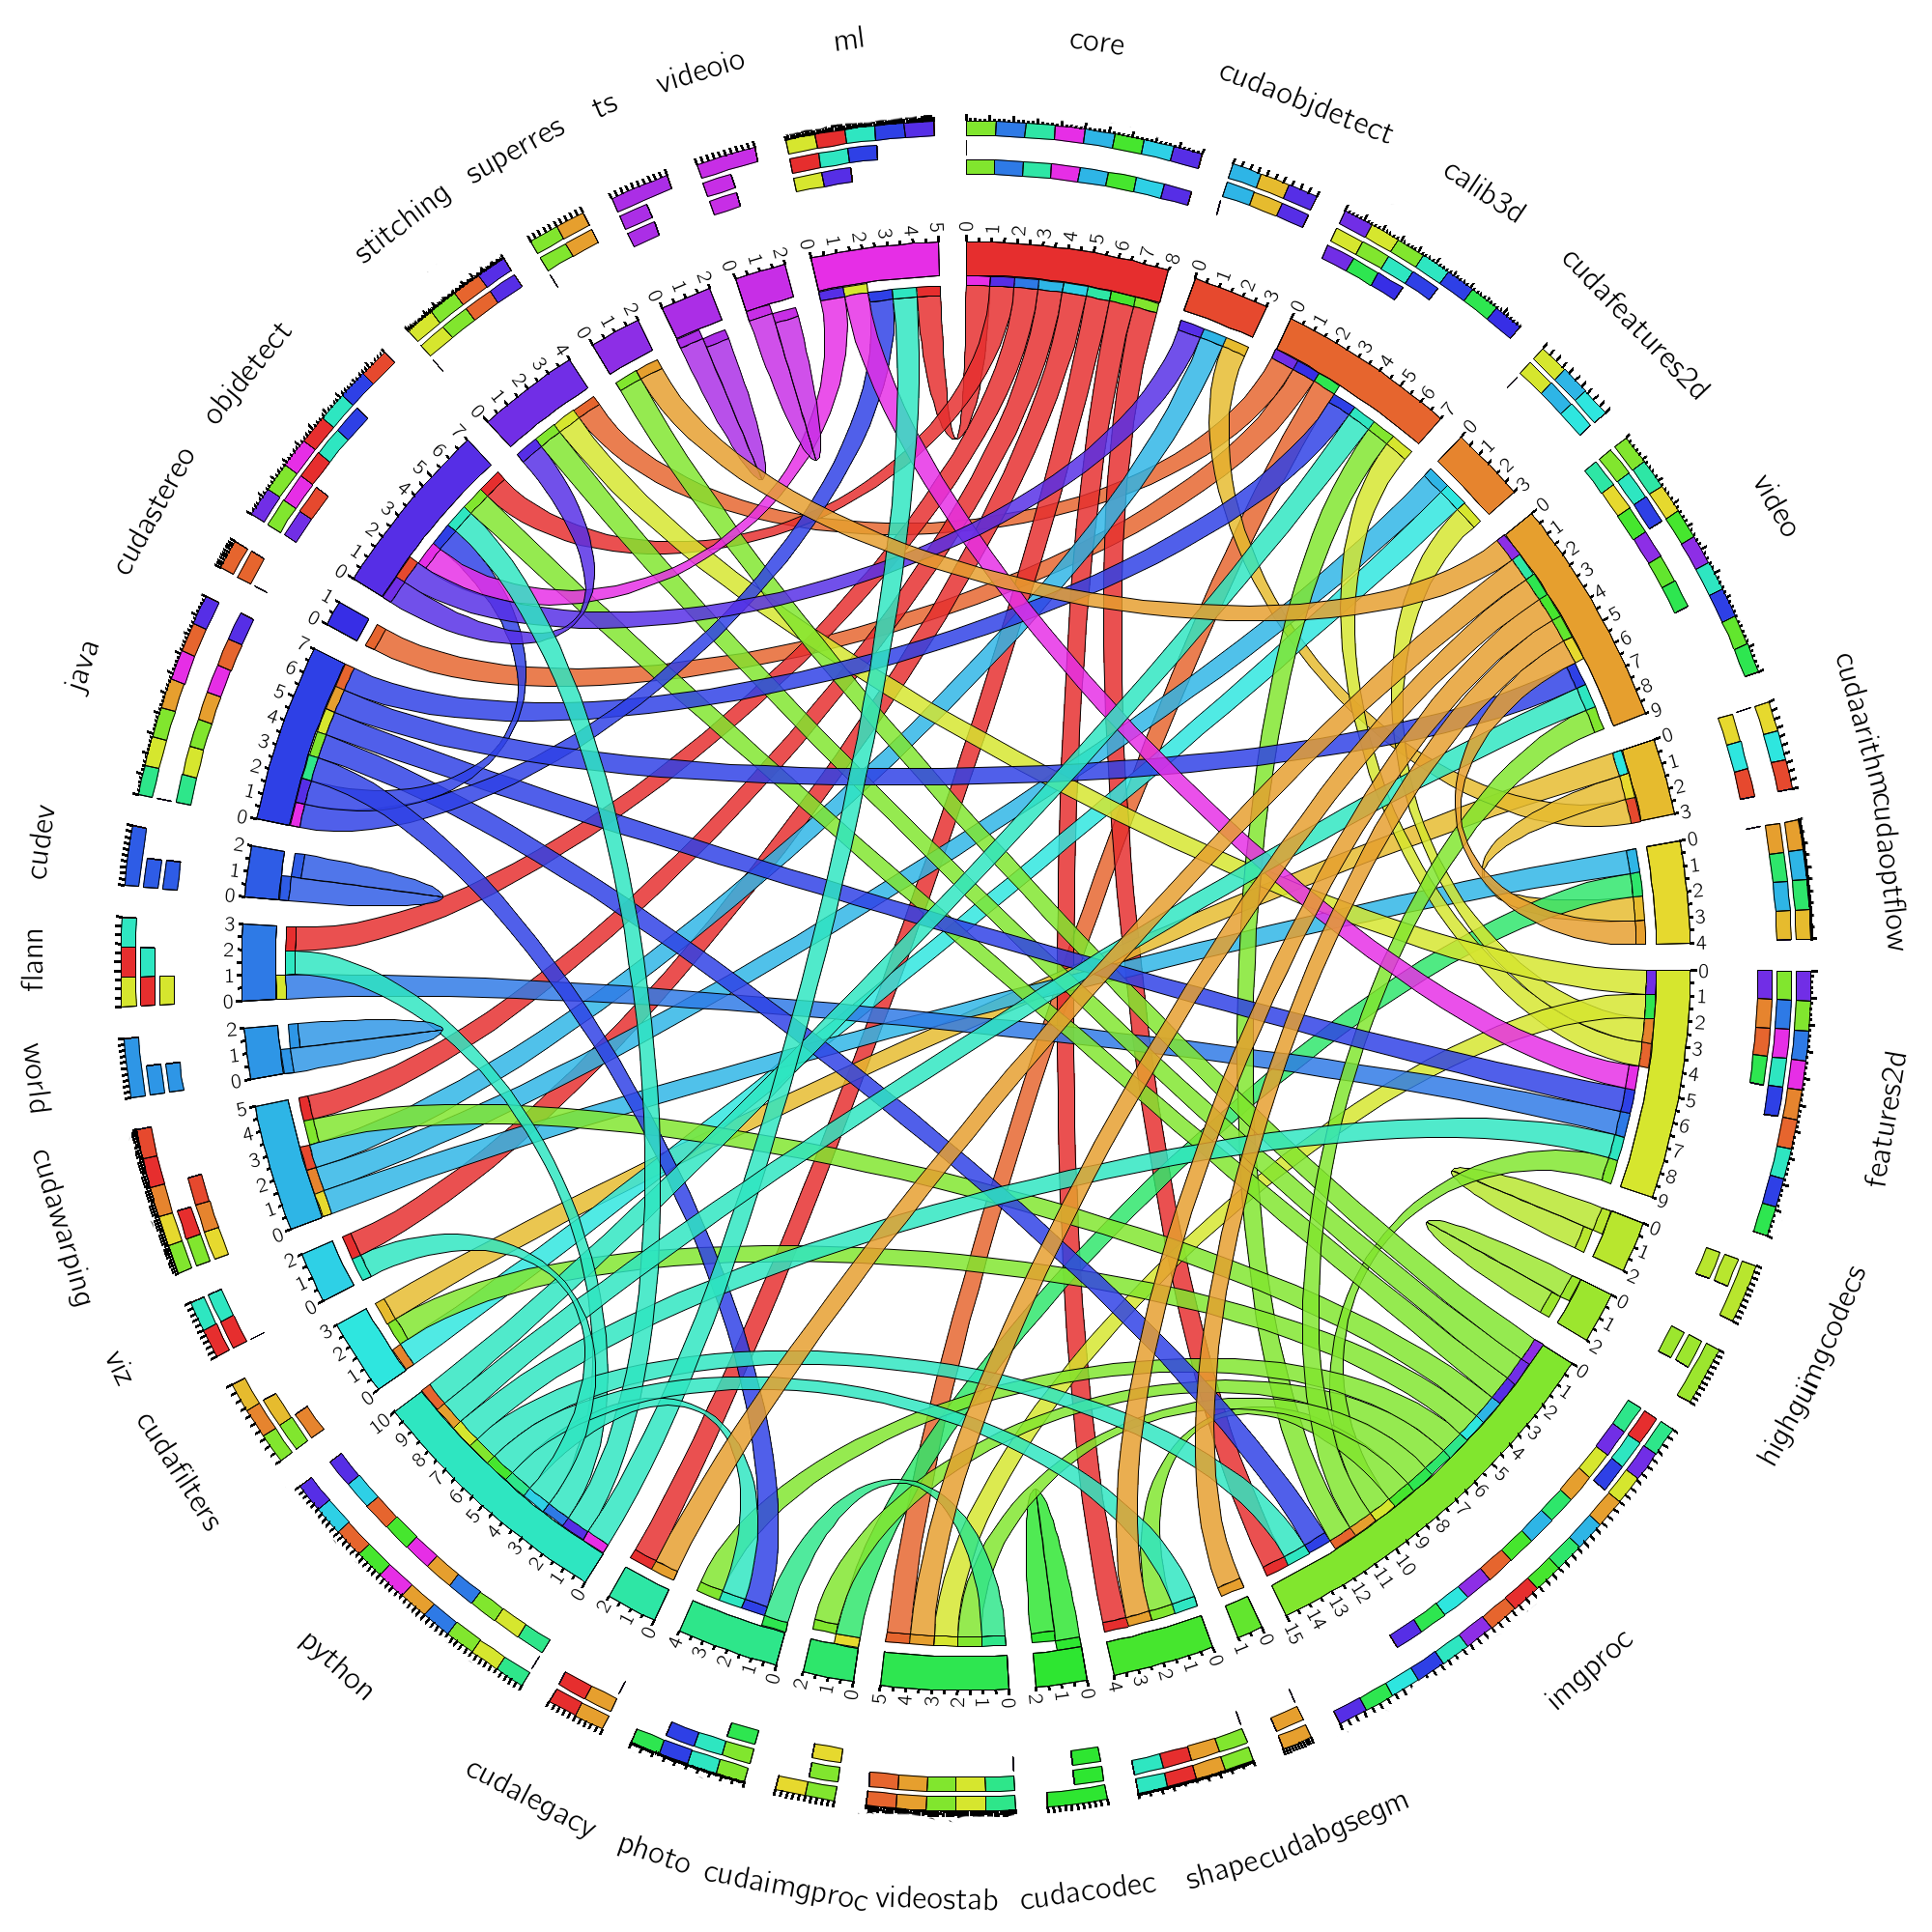
\includegraphics{Figures/ModulesStructure.png}}
     \caption{\label{Figure::ModulesStructure} Modules Interconnection Structure}
\end{figure}
Because of its complex nature, we will zoom into the architecture a little bit and understand one such important module of OpenCV among the 15 most important modules through all the 4+1 views' from here on:
\begin{itemize}
         \item Image Stitching Module (stitching.): Famously used to create panorama images \cite{6896208}. \index{panorama} 
\end{itemize}
The idea is to understand this one module which in-turn sort of explains the rest of the OpenCV modules in OpenCV's architecture. \\\\
Below is a Package Diagram of Image Stitching Module:\\\\
The diagram includes 3 levels:
\begin{enumerate}
         \item 1st Level: It is the OpenCV package that contains all modules.
         \item 2nd Level: It shows how the Image Stitching module is Interacting with other modules in OpenCV package.
         \item 3rd Level: Shows the functions present in Image Stitching module and the other two modules.
\end{enumerate}

\begin{figure}[H]
     \centering
     \scalebox{0.5}{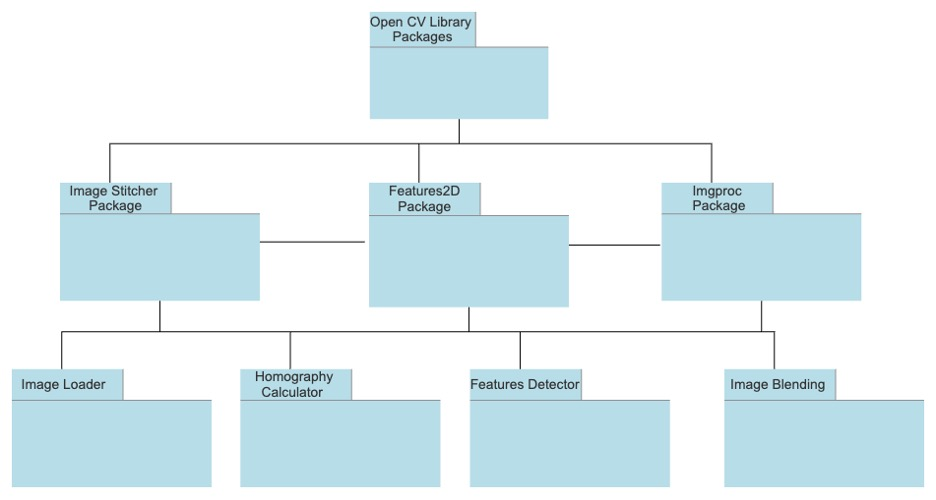
\includegraphics{Figures/PackageDiagram.jpg}}
     \caption{\label{Figure::ImageStitcherPackageDiagram
} Image Stitcher Package Diagram}
\end{figure}

\subsubsection{Functions\label{subsubSection::Functions}}
\begin{enumerate}
         \item Image Loader: It is used to load and prepare the images in Image Stitching package for stitching process.
         \item Homography Calculator: It is used to calculate a homography matrix between two sets of corresponding points in an image. \index{Homography}
         \item Features Detector: It is used to identify and extract distinctive features or points of interest from an image.
         \item Image Blending: It is the process of combining two or more images to create a single composite image that preserves the important information from each input image. \index{Image Blending}
\end{enumerate}
\pagebreak

\subsection{Use Case View\label{subSection::UserCaseView}} \index{User Case View}
The use case view is an architectural view that focuses on describing the system's functionality from the perspective of its users or external actors.\\\\
     In our case we will consider the following:
     \begin{itemize}
         \item Perspective: End users
         \item Stage: Putting it alltogether
         \item Concerns: Understandability, usability
         \item Focus: Feature decomposition
         \item Artefact: Use-case diagram
     \end{itemize}

\subsubsection{Use Case Diagram\label{subsubSection::UseCaseDiag}}
\begin{figure}[H]
     \centering
     \scalebox{0.68}{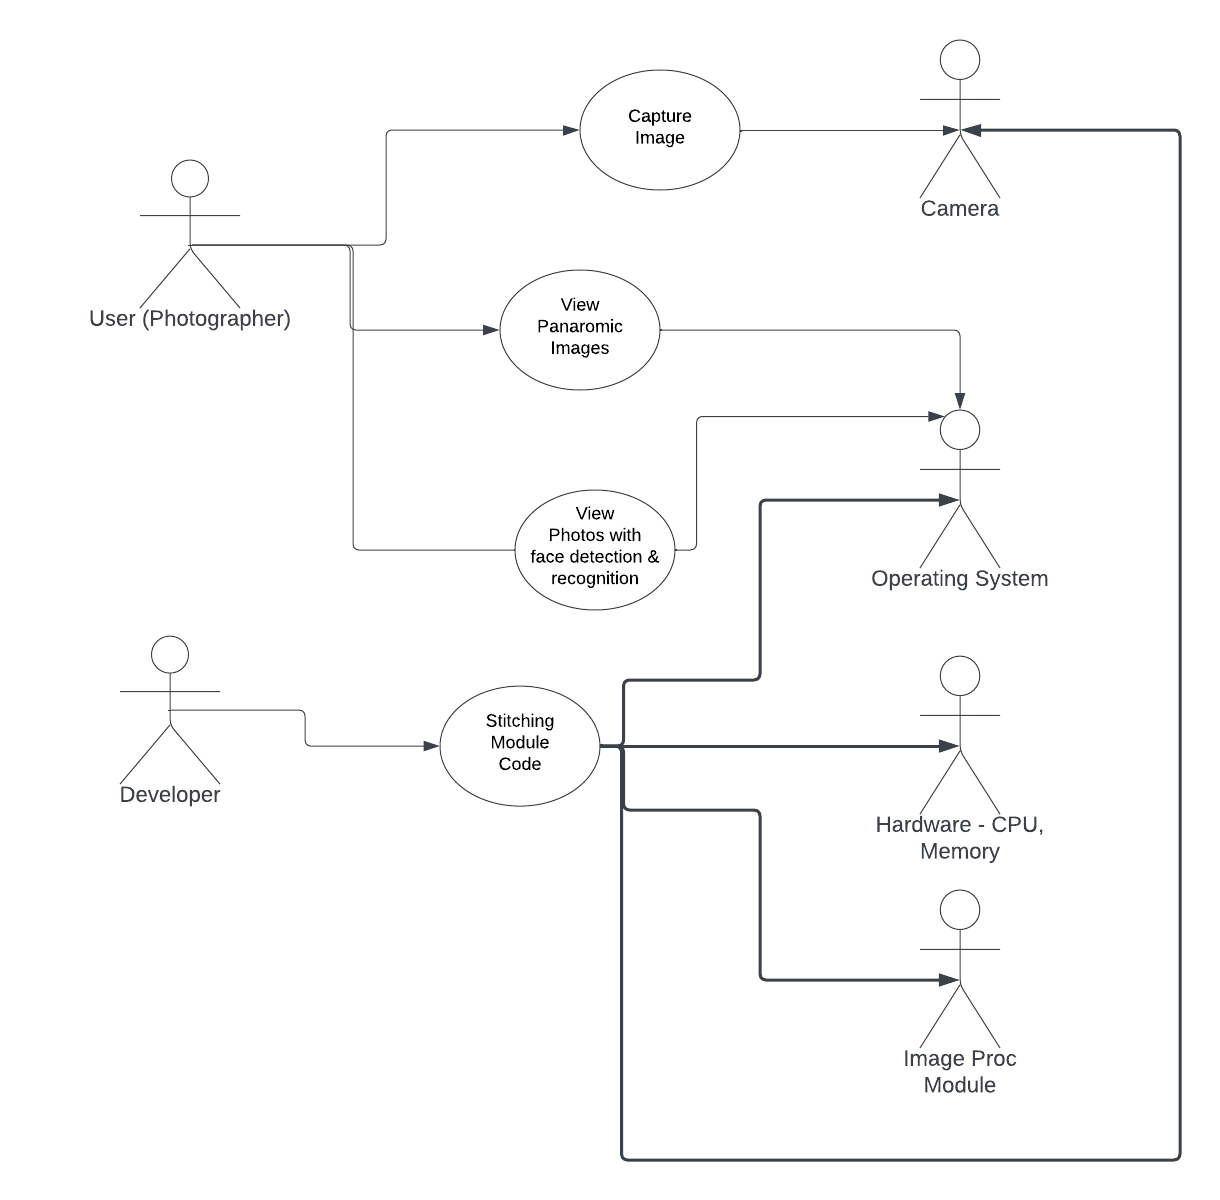
\includegraphics{Figures/Use Case Diagram of ImageStitchingModule.png}}
     \caption{\label{Figure::UseCaseDiagram
} Use Case Diagram for Image Stiching Module \cite{lucidchart}}
\end{figure}

We have the following in our diagram:
\begin{enumerate}
         \item Actors: Two actors \index{Actors}
         \begin{enumerate}
         \item User: Photographer has 3 use cases:- \index{Photographer}
             \begin{enumerate}
             \item To capture images
             \item View panaromic images
             \item View photos with face detection and recognition.
             \end{enumerate}
         \item Developer has 1 use case:- \index{Developer}
             \begin{enumerate}
             \item Develop stitching module code
             \end{enumerate}
\end{enumerate}
         \item Use Cases: Four use cases 
         \begin{enumerate}
             \item To capture images
             \item View panaromic images
             \item View photos with face detection and recognition.
             \item Develop stitching module code
         \end{enumerate}

         \item External Actors: Four external actors
         \begin{enumerate}
             \item Camera: Facilitates in capturing images \index{Camera}
             \item Operating System: Used by both User and developer for their use cases \index{Operating System}
             \item Hardware Components: CPU, Memory \index{CPU} \index{Memory}
             \item Image Proc Module: Provides a wide range of functions and algorithms for manipulating and enhancing images.
         \end{enumerate}
         
\end{enumerate}


\pagebreak

\subsection{Logical View\label{subSection::LogicalView}} \index{Logical View}
The logical view is an architectural view that focuses on representing the high-level structure and organization of the system's functionality and behavior. It provides an abstraction of the system's functionality and its relationships, without delving into implementation details. \\\\
     In our case we will consider the following:
     \begin{itemize}
         \item Perspective: Analysts, Designers Stage: Requirement analysis \index{Analysts}
         \item Focus: Object oriented decomposition
         \item Concerns: Functionality
         \item Artefacts: Class diagram \cite{UMLdiagram}
     \end{itemize}

\begin{figure}[H]
     \centering
     \scalebox{0.6}{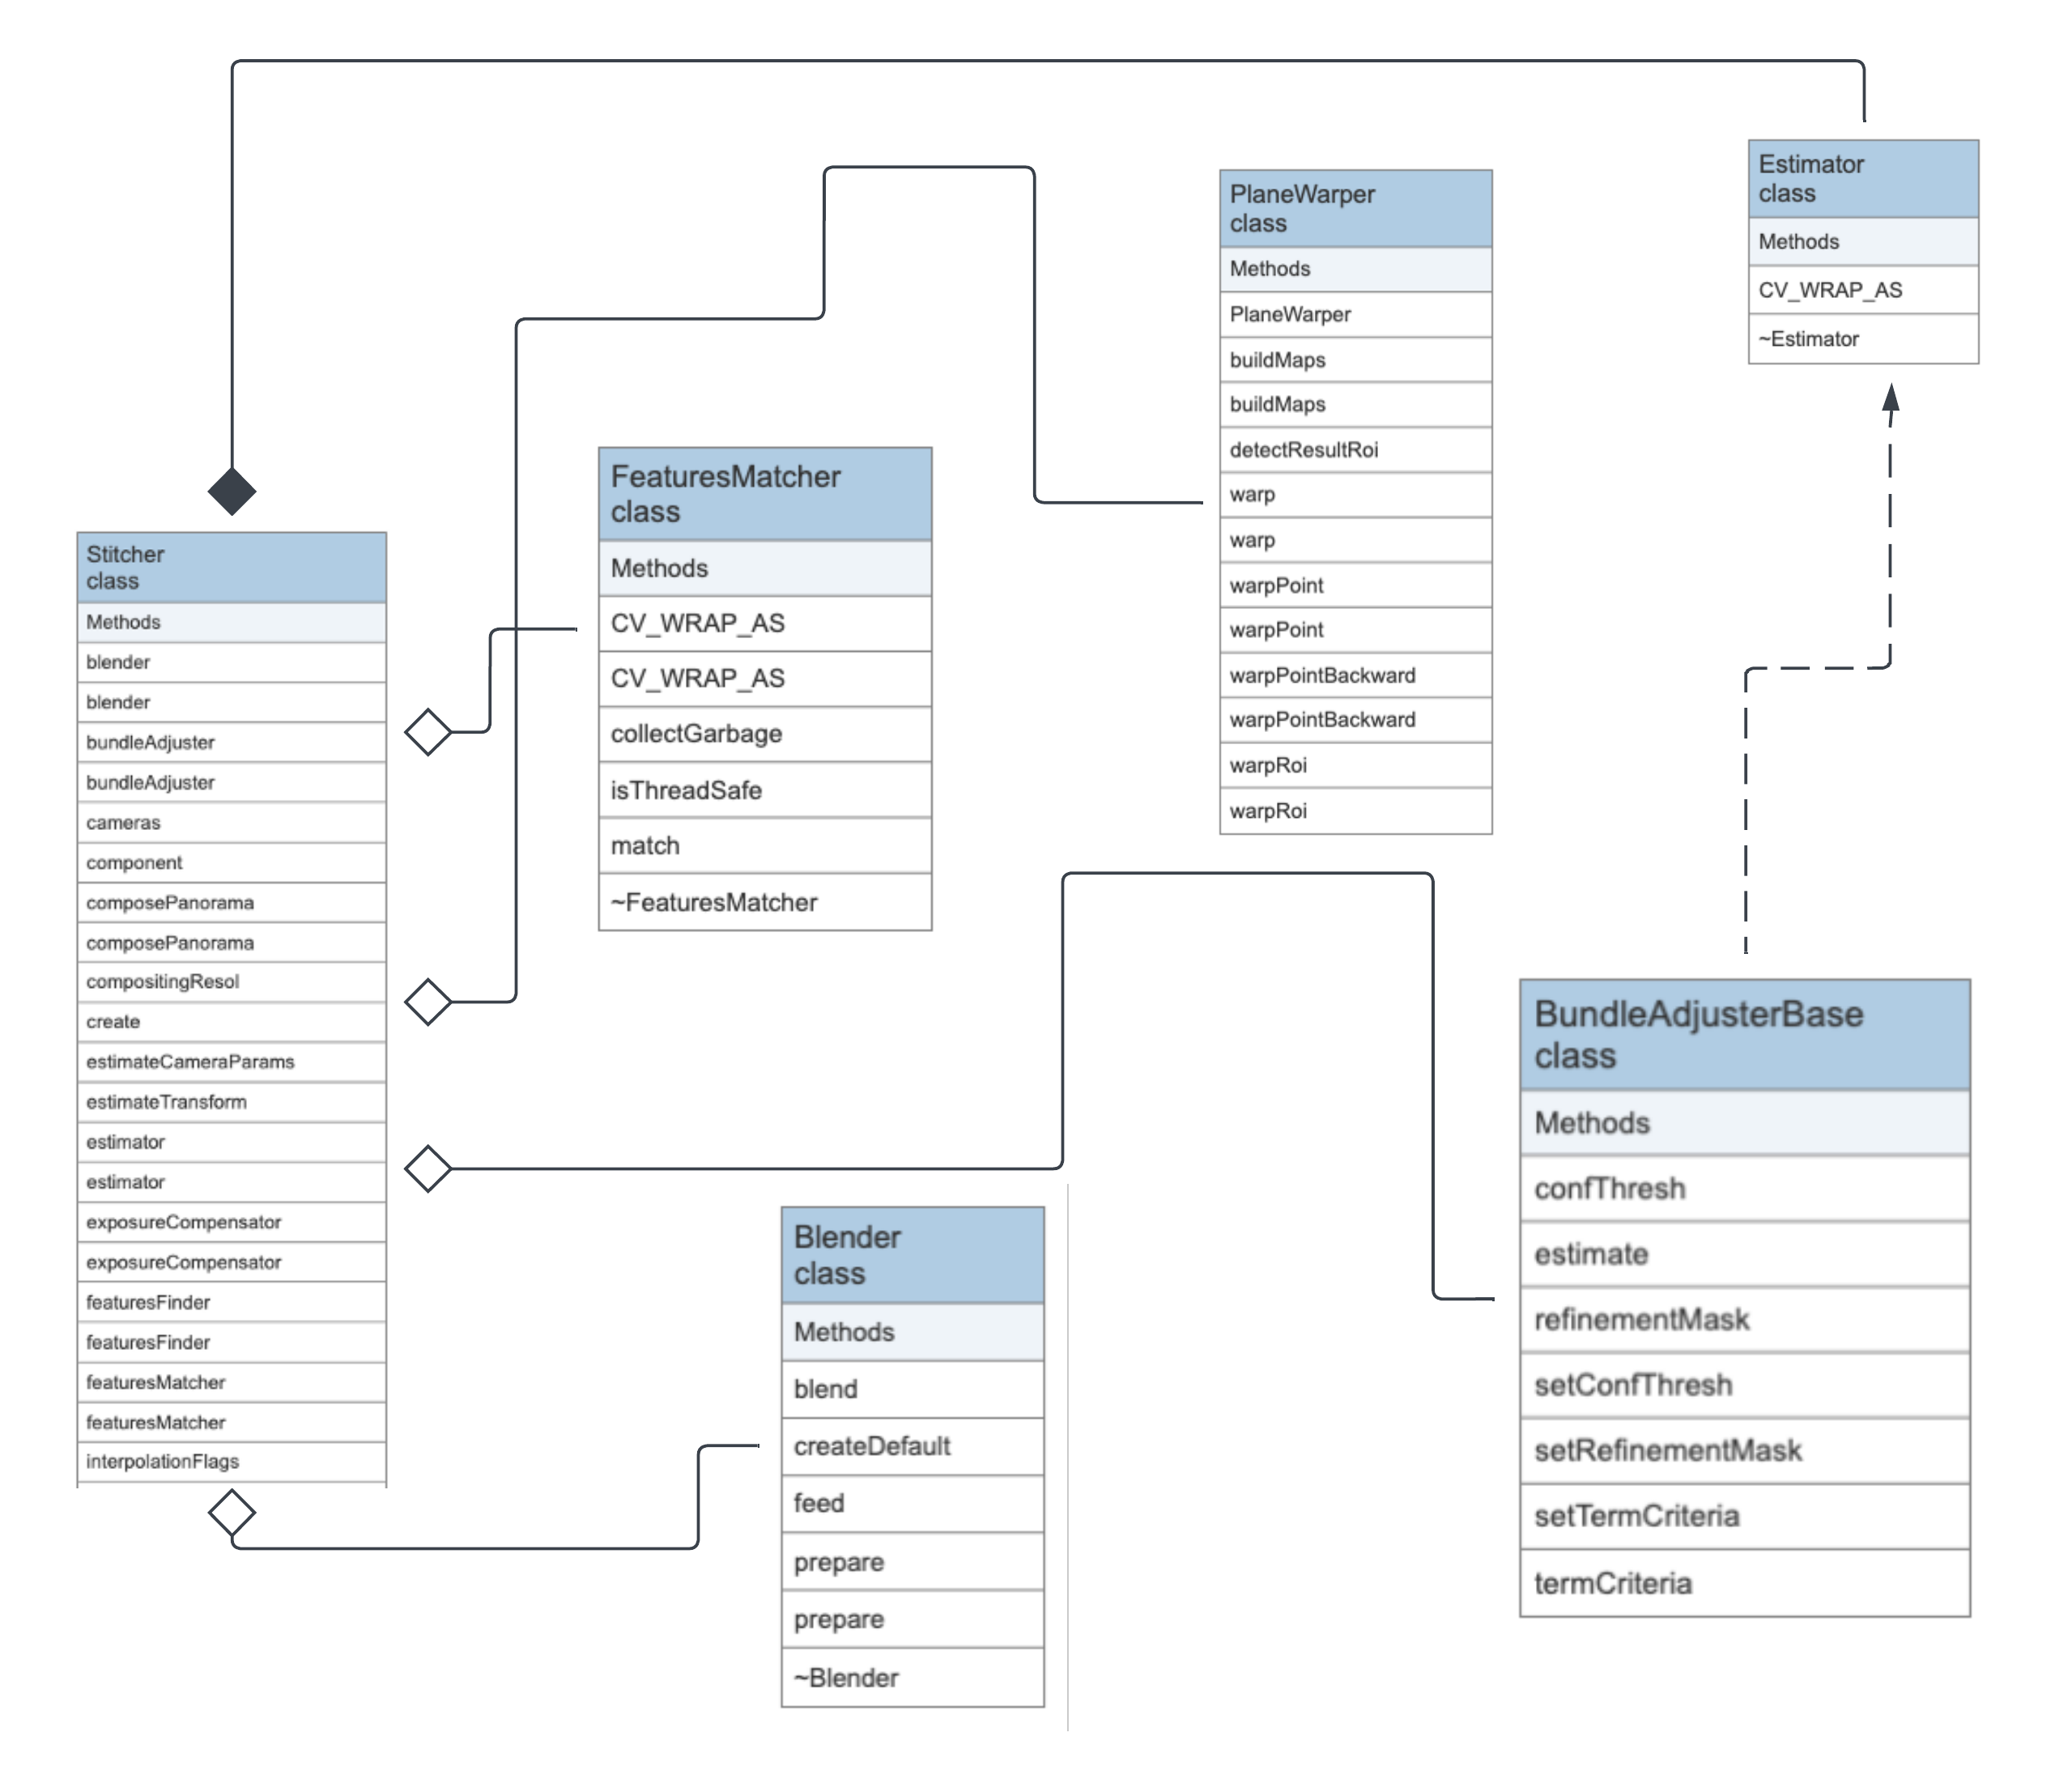
\includegraphics{Figures/ClassDiagram.png}}
     \caption{\label{Figure::BriefOverview} Class Diagram of Image Stitching Module \cite{smartdraw}}
\end{figure}
The logical view of OpenCV's Image Stitching module describes the system's functionality and the relationships between its components. The module consists of several classes, including the Stitcher class, Features Matcher class, Plane Warper class, Blender class, BundleAdjusterBaseClass, and Estimator class. Here is a brief description of each class and how they depend on each other:
\begin{enumerate}
    \item Stitcher class: The Stitcher class is the main class in the Image Stitching module. It provides the functionality to stitch multiple images together to create a panoramic image. The Stitcher class uses other classes in the module to perform various tasks, such as feature detection, feature matching, and image blending.
    \item Features Matcher class: The Features Matcher class is responsible for detecting and matching features in the input images. It uses various algorithms to detect and match features, such as the SIFT algorithm and the SURF algorithm.
    \item Plane Warper class: The Plane Warper class is responsible for warping the input images to a common plane. It uses various algorithms to perform the warping, such as the Homography algorithm and the Affine algorithm.
    \item Blender class: The Blender class is responsible for blending the warped images together to create a seamless panoramic image. It uses various algorithms to perform the blending, such as the Multi-band blending algorithm and the Feather blending algorithm.
    \item BundleAdjusterBaseClass: The BundleAdjusterBaseClass is responsible for adjusting the parameters of the stitching process to improve the quality of the output image. It uses various algorithms to adjust the parameters, such as the Levenberg-Marquardt algorithm and the Gauss-Newton algorithm.
    \item Estimator class: The Estimator class is responsible for estimating the camera parameters of the input images. It uses various algorithms to estimate the parameters, such as the RANSAC algorithm and the Least Squares algorithm.\\
\end{enumerate}
These classes depend on each other in a hierarchical manner. The Stitcher class is the main class that uses the other classes to perform various tasks. The Features Matcher class and the Estimator class are used by the Stitcher class to detect and match features and estimate camera parameters, respectively. The Plane Warper class is used by the Stitcher class to warp the input images to a common plane. The Blender class is used by the Stitcher class to blend the warped images together to create a seamless panoramic image. Finally, the BundleAdjusterBaseClass is used by the Stitcher class to adjust the parameters of the stitching process to improve the quality of the output image. Overall, these classes work together to provide the functionality of the Image Stitching module in OpenCV.
\pagebreak


\subsection{Process View\label{subSection::ProcessView}}
The process view is an architectural view that focuses on illustrating the runtime behavior and concurrency aspects of a system. It provides a perspective on how the system's functionality is executed and how different components or processes interact and collaborate during runtime.\\\\
     In our case we will consider the following:
     \begin{itemize}
         \item Perspective: System Integrators \index{System Integrators}
         \item Stage: Design
         \item Focus: Process decomposition
         \item Concerns: Performance, scalability, throughput \index{throughput}
         \item Artefacts: Sequence diagram \index{Sequence diagram}
     \end{itemize}
     
\subsubsection{Sequence Diagram\label{subsubSection::SequenceDiag}}
\begin{figure}[H]
     \centering
     \scalebox{0.38}{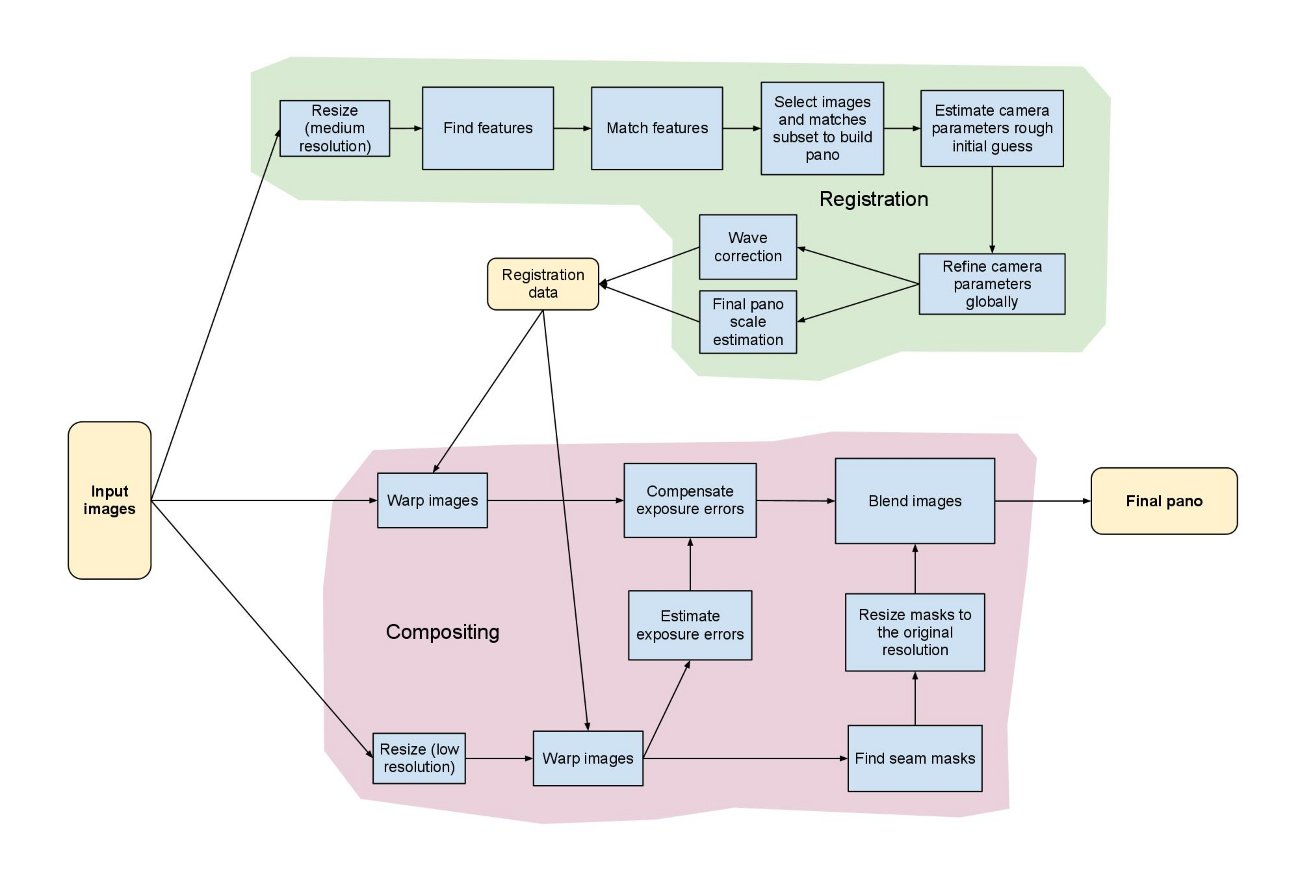
\includegraphics{Figures/StitchingPipeline.jpg}}
     \caption{\label{Figure::StitchingPipeline} Sequence Diagram of Image Stitching Module} \index{Stitching Pipeline}
\end{figure}
The process view of OpenCV's Image Stitching module describes the system's behavior and how it responds to external events. The module performs several operations to stitch multiple images together to create a panoramic image. Here is a brief description of each operation and the steps involved:
\begin{enumerate}
    \item Step 1 - Input Images:\\ The first operation is to input the images that need to be stitched together. These images are typically captured using a camera or downloaded from a source.

    \item Step 2 - Registration:\\ The second operation is registration, which involves several steps:
    \begin{itemize}
        \item Resize (medium resolution): The input images are resized to a medium resolution to reduce the computational complexity of the feature detection and matching algorithms.
        \item Find features: The feature detection algorithm is used to detect features in the input images, such as corners, edges, and blobs.
        \item Match features: The feature matching algorithm is used to match the features between the input images.
        \item Select images and matches subset to build panorama: The input images and their corresponding feature matches are selected to build the panorama.
        \item Estimate camera parameters rough initial guess: The camera parameters of the input images are estimated using a rough initial guess.
        \item Refine camera parameters globally: The camera parameters are refined globally using a bundle adjustment algorithm.
        \item Wave correction: The wave correction algorithm is used to correct the distortion caused by the camera lens.
        \item Final panorama scale estimation: The final scale of the panorama is estimated based on the camera parameters and the input images.
    \end{itemize}

    \item Step 3 - Registration data :\\ The registration data, including the camera parameters and the warped images, are passed to the compositing operation.

    \item Step 4 - Compositing:\\ The final operation is compositing, which involves several steps:
    \begin{itemize}
        \item Warp images: The warped images are transformed to a common coordinate system using the estimated camera parameters.
        \item Estimate exposure errors: The exposure errors in the input images are estimated using an exposure estimation algorithm.
        \item Compensate exposure errors: The exposure errors in the input images are compensated using an exposure compensation algorithm.
        \item Resize (low resolution): The final panoramic image is resized to a low resolution for display or storage purposes.
        \item Warp images: The warped images are transformed again to the original resolution.
        \item Find seam masks: The seam masks are found using a seam finding algorithm.
        \item Resize masks to original resolution: The seam masks are resized to the original resolution.
        \item Blend images: The blended image is created by blending the warped images together using a blending algorithm.
    \end{itemize}
    \item Step 5 - Final panorama:\\ The final panoramic image is created by combining the blended image and the seam masks.
\end{enumerate}
Overall, the process view of OpenCV's Image Stitching module describes the system's behavior and how it responds to external events, such as input images and user requests. The module performs several operations, including registration and compositing, to stitch multiple images together to create a beautiful panoramic image.
\pagebreak

\subsection{Deployment View\label{subSection::DeploymentView}}
The deployment view is an architectural view that focuses on illustrating how the software components of a system are deployed and distributed across hardware resources. It provides a representation of the physical infrastructure and deployment topology of the system.\\\\ \index{Deployment View}
     In our case we will consider the following:
     \begin{itemize}
         \item Perspective: System Engineers
         \item Stage: Design
         \item Focus: Map software to hardware
         \item Concerns: System topology, delivery, installation, communication
         \item Artefacts: Deployment diagram
     \end{itemize}

\subsubsection{Deployment Diagram\label{subsubSection::DeploymentDiag}}
\begin{figure}[H]
     \centering
     \scalebox{0.9}{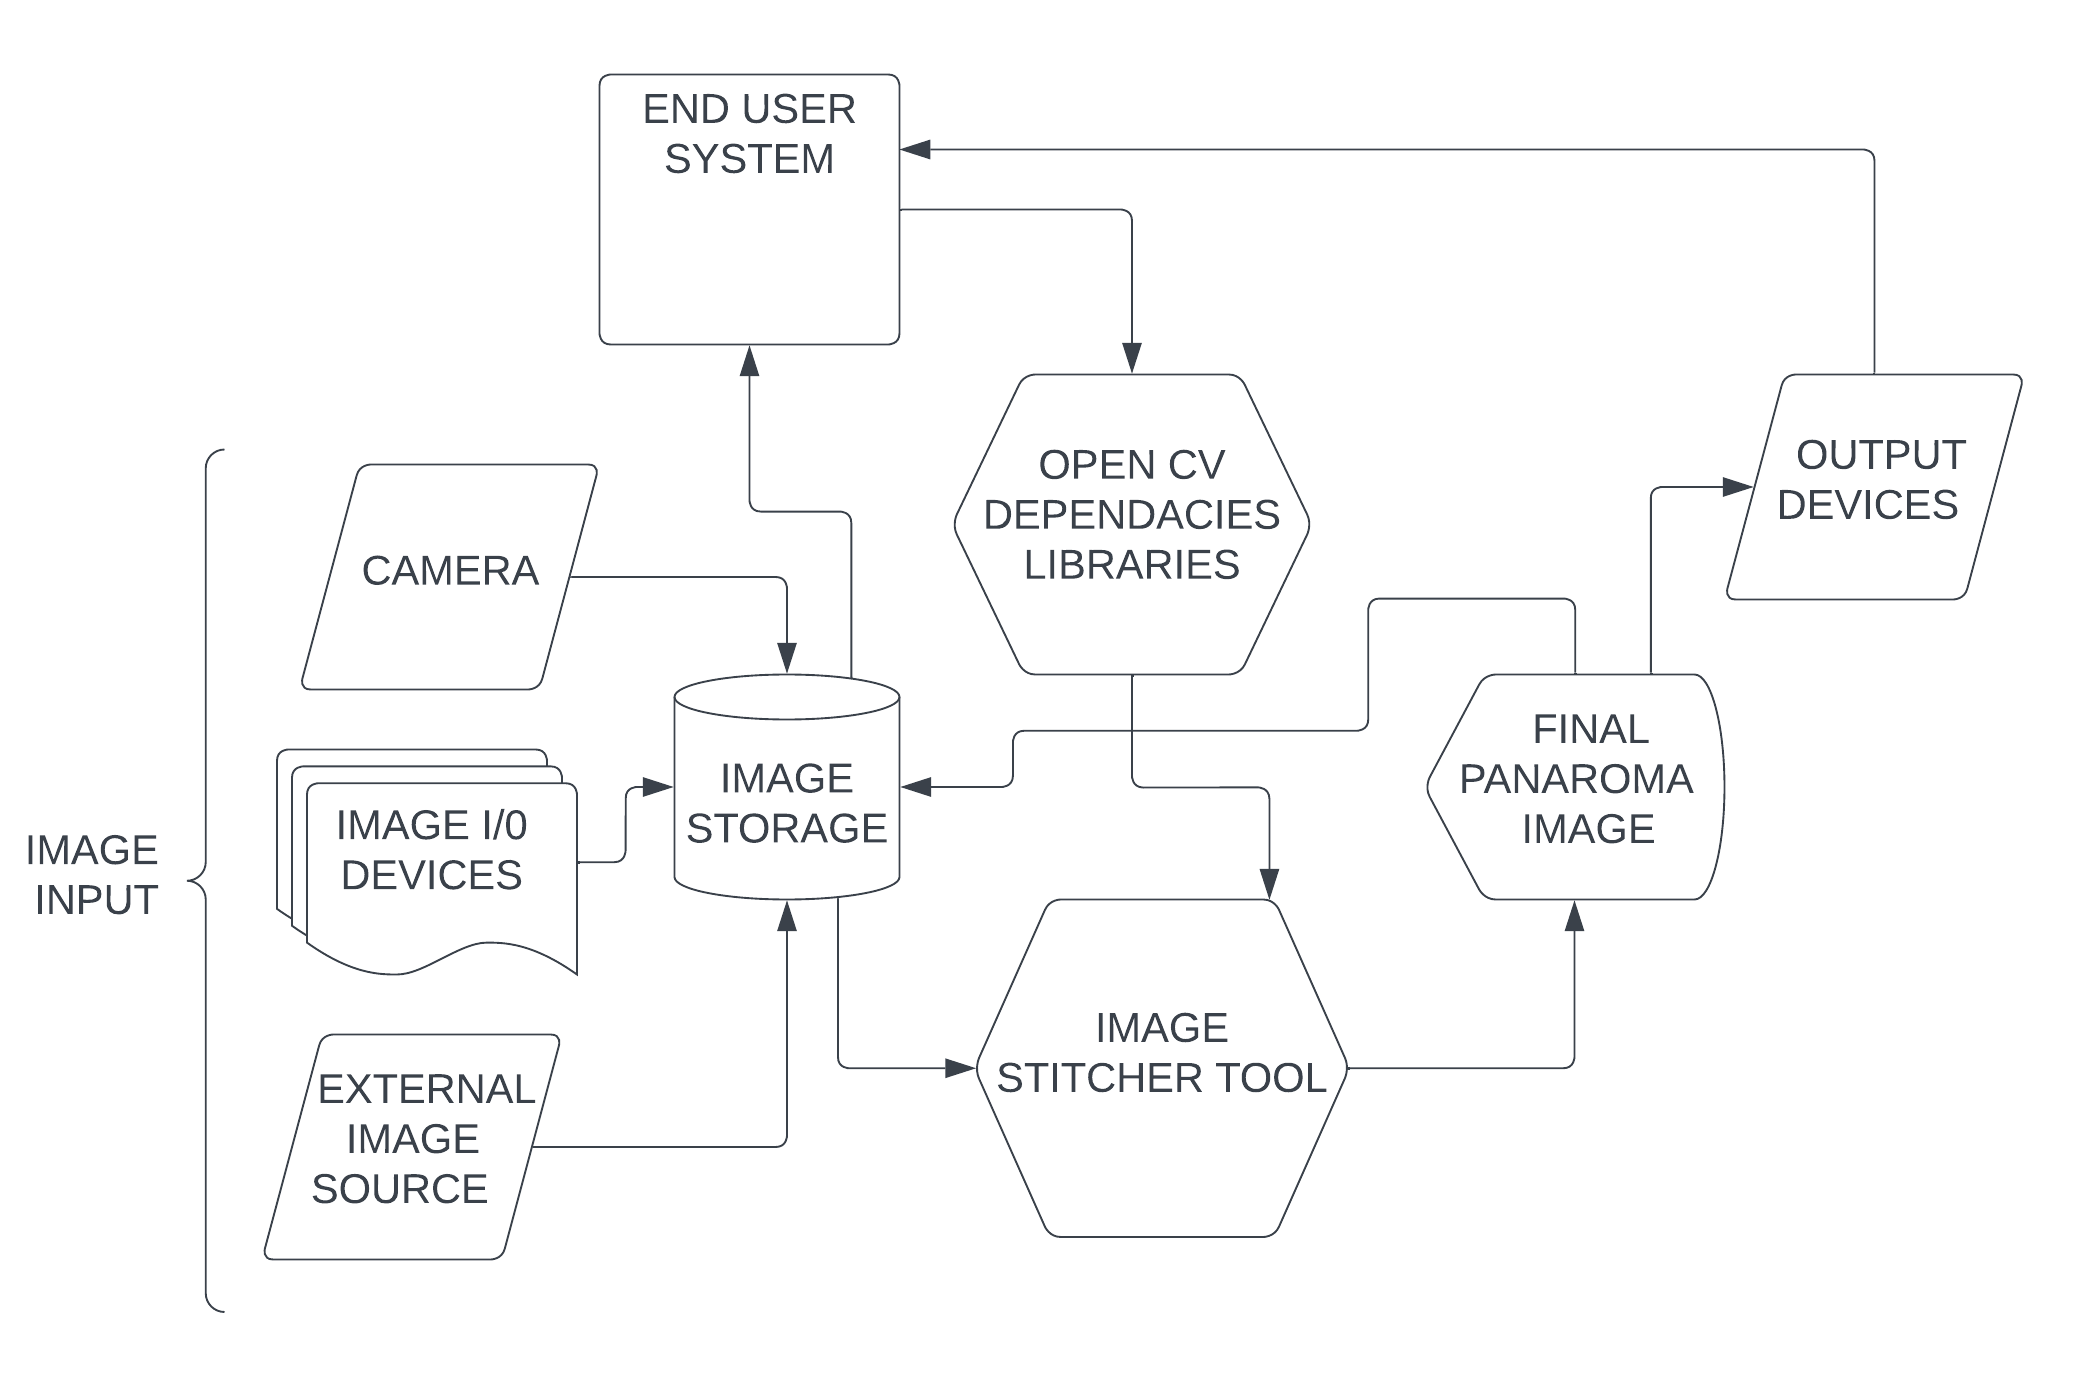
\includegraphics{Figures/DeploymentDiagram.png}}
     \caption{\label{Figure::DeploymentDiagram} Deployment Diagram of Image Stitching Module}
\end{figure}
The deployment view of OpenCV's image stitching module involves several components that work together to produce a final panorama output image: 
\begin{enumerate}
    \item Image input: The images that need to be stitched together.
    \begin{itemize}
        \item Camera: This is the device that captures the images that will be stitched together. 
        \item Image input/output devices: These are devices that can be used to input or output images, such as USB drives or SD cards. 
        \item External image source: This component refers to any external source of images that can be used as input for the stitching process.
    \end{itemize}
    \item Image storage database: This component is responsible for storing the images that will be used for stitching. It can be a local or remote database.

    \item OpenCV libraries / dependencies: This component includes all the necessary libraries and dependencies required for the image stitching module to function properly.

    \item Image Stitching module of OpenCV: This is the core component of the deployment view. It is responsible for stitching the input images together to produce a final panorama output image.

    \item Final panorama output image: This is the output of the image stitching module. It is the final image that is produced after the input images have been stitched together.

    \item Output devices: These are devices that can be used to output the final panorama image, such as a monitor or a printer.

    \item End-user system: This component refers to the system that the end-user will be using to access the image stitching module. It can be a desktop computer, a laptop, or a mobile device.
\end{enumerate}
Overall, the deployment view of OpenCV's image stitching module involves several components that work together to produce a final panorama output image. The input images can come from various sources, and the final output can be displayed on different output devices. The image stitching module is the core component that stitches the input images together, and the end-user system is the system that the end-user will be using to access the module.
\subsubsection{OpenCV Installation Dependencies\label{subsubSection::opencvInstallation}}
To install OpenCV on a system, there are several dependencies that need to be installed first. The specific dependencies required may vary depending on the operating system and the version of OpenCV being installed. Here is a general list of dependencies that are commonly required:
\begin{enumerate}
    \item CMake: This is a cross-platform build system that is used to build OpenCV from source.
    \item Git: This is a version control system that is used to download the OpenCV source code.
    \item GCC: This is a compiler that is used to compile the OpenCV source code.
    \item Python: OpenCV has a Python interface, so Python needs to be installed on the system.
    \item NumPy: This is a Python library that is used for numerical computing. It is required for the Python interface of OpenCV.
    \item libjpeg: This is a library for reading and writing JPEG files. It is required for the imgcodecs module of OpenCV.
    \item libpng: This is a library for reading and writing PNG files. It is required for the imgcodecs module of OpenCV.
    \item libtiff: This is a library for reading and writing TIFF files. It is required for the imgcodecs module of OpenCV.
    \item libjasper: This is a library for reading and writing JPEG-2000 files. It is required for the imgcodecs module of OpenCV.
    \item libwebp: This is a library for reading and writing WebP files. It is required for the imgcodecs module of OpenCV.
    \item OpenEXR: This is a library for reading and writing high dynamic range (HDR) images. It is required for the imgcodecs module of OpenCV.
    \item TBB: This is the Intel Threading Building Blocks library, which is used for parallel processing. It is required for the performance optimization of OpenCV.
    \item Eigen: This is a C++ template library for linear algebra. It is used for the computation of homography matrices in the image stitching process.
    \item CUDA: This is a parallel computing platform and programming model developed by NVIDIA. It is used for GPU acceleration in the image stitching process.
    \item OpenCL: This is an open standard for parallel programming of heterogeneous systems. It is used for GPU acceleration in the image stitching process.
\end{enumerate}
\pagebreak

\section{Summary of 4+1 View:\label{Section::Overview}}
Each view provides a distinct perspective on the OpenCV architecture, allowing stakeholders to understand and analyze the system from different angles. This 4+1 view model helps in capturing the functional, development, process, physical, and use case aspects of the OpenCV backend architecture.\\\\ \index{Backend}
Here is a diagram to showcase a brief overview of what we covered:

\begin{figure}[H]
     \centering
     \scalebox{0.23}{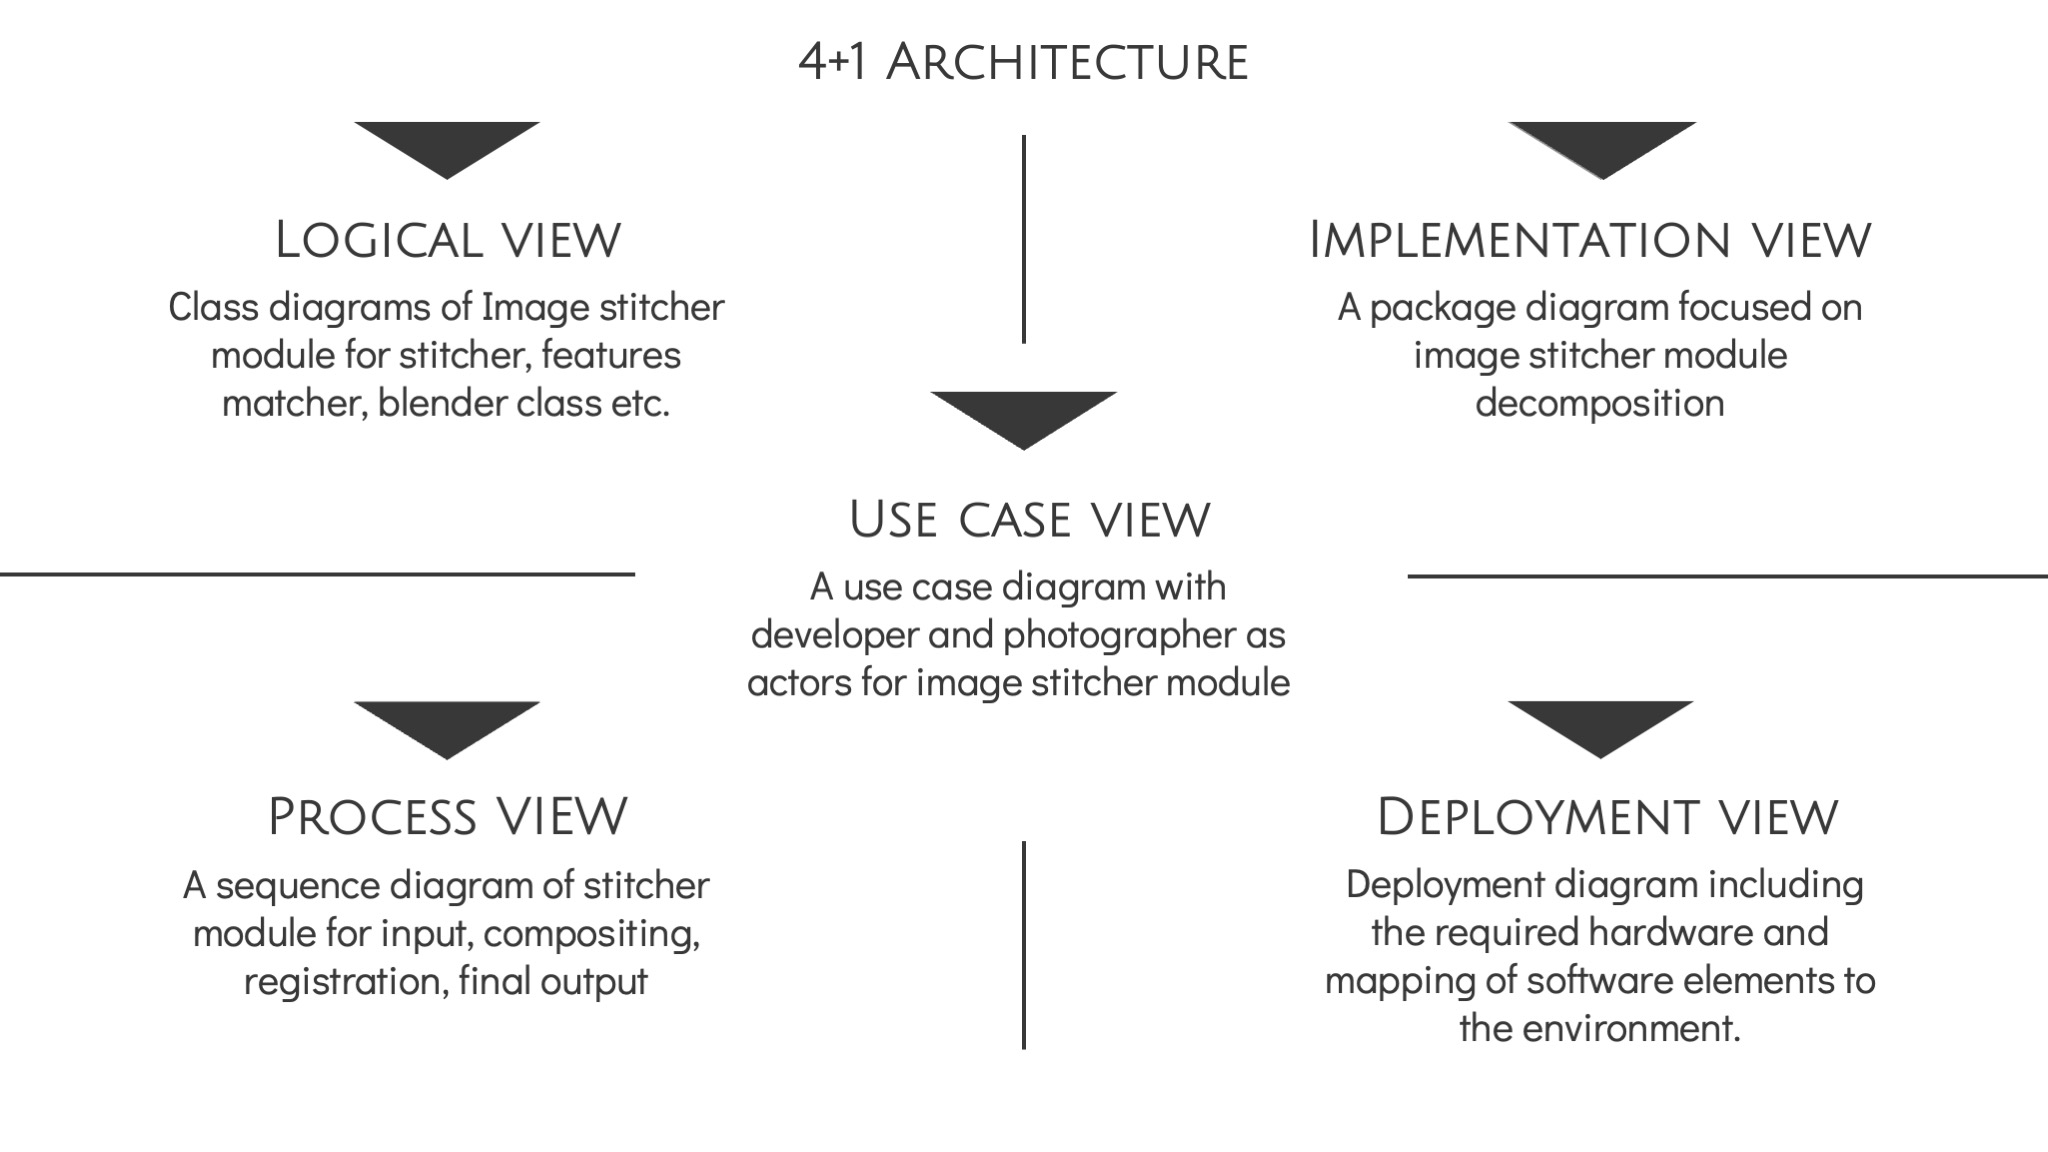
\includegraphics{Figures/BriefOverview.jpg}}
     \caption{\label{Figure::BriefOverview} 4+1 Overview}
\end{figure}
\par{The purpose of using the 4+1 view model for OpenCV's Image Stitching module is to provide a comprehensive understanding of the system's architecture from multiple perspectives. This approach helps to ensure that the system is designed and implemented in a way that meets the needs and requirements of its stakeholders, while also addressing potential risks and quality issues. \index{4+1 view}\\
\\
The Logical View provides a high-level overview of the system's functionality and the relationships between its components. This view focuses on the system's data and functionality, and how they are organized and structured. It helps stakeholders to understand the system's overall purpose and how it achieves its goals.\\
\\
The Process View describes the system's behavior and how it responds to external events. This view focuses on the system's processes and how they interact with each other and with external systems. It helps stakeholders to understand how the system works and how it responds to different inputs and events.\\
\\
The Implementation View describes the system's development environment and how it is organized. This view focuses on the system's development tools, processes, and methodologies. It helps stakeholders to understand how the system is developed and maintained, and how changes are made to the system over time.\\
\\
The Deployment View describes the system's physical architecture and how it is deployed. This view focuses on the system's hardware and software components, and how they are connected and configured. It helps stakeholders to understand how the system is deployed and how it interacts with other systems and devices.\\
\\
The Use Case View describes the system's functionality from the perspective of its users. This view focuses on the system's use cases and how they are implemented in the system. It helps stakeholders to understand how the system is used and how it meets the needs and requirements of its users.
\vspace{20pt}\\
Overall, the 4+1 view model provides a comprehensive understanding of the OpenCV Image Stitching module's architecture from multiple perspectives, helping stakeholders to understand the system's functionality, behavior, development environment, physical architecture, and user requirements. This understanding is essential for ensuring that the system is designed and implemented in a way that meets the needs and requirements of its stakeholders, while also addressing potential risks and quality issues.
}







\bibliography{bibfile}
%\bibliographystyle{unsrt}
\bibliographystyle{IEEEtran}

%% Initial version by Darian Muresan, Ph.D.
% Edit and adjust as needed.

\documentclass[12pt]{cornell}

% add index support
\makeindex

% graphing programs
\usepackage{color}
\usepackage{psfrag}
\usepackage{verbatim}
\usepackage{fancyhdr}
%\usepackage{titlesec}
\usepackage{fancyvrb} 
% hyperlink programs
\usepackage[pdfmark, 
breaklinks=true, 
colorlinks=true,
citecolor=blue,
linkcolor=blue,
menucolor=black,
pagecolor=black,
urlcolor=blue
]{hyperref} % links in pdf
%\usepackage[colorlinks]{hyperref} % links in dvi
\usepackage{listings}
\usepackage{amsfonts} 
\usepackage{amssymb} 
%\usepackage{tabto}

\usepackage{tabularx,colortbl}
\usepackage[chapter]{algorithm} 
\usepackage{algorithmic} 
\usepackage{blindtext}
\usepackage{imakeidx}


\definecolor{DarkGreen}{rgb}{0,0.6,0}
\definecolor{mygreen}{rgb}{0,0.6,0}
\definecolor{mygray}{rgb}{0.5,0.5,0.5}
\definecolor{mymauve}{rgb}{0.58,0,0.82}

\usepackage{tocloft}
\usepackage{amsmath}
\usepackage{tcolorbox}
\usepackage{enumitem}
\usepackage{longtable}
%\usepackage{textcomp}
\usepackage{txfonts}

%part for \part titles
%chap for \chapter titles
%sec for \section titles
%subsec for \subsection titles
%subsubsec for \subsubsection titles
%para for \paragraph titles
%subpara for \subparagraph titles
%fig for figure \caption titles
%subfig for subfigure \caption titles
%tab for table \caption titles
%subtab for subtable \caption titles

% update chapter number spacing
\setlength{\cftchapnumwidth}{2em}
\setlength{\cftsecnumwidth}{2.5em}
\setlength{\cftsubsecnumwidth}{3.5em}
\setlength{\cftsubsubsecnumwidth}{4.5em}

\addtolength{\cftsecindent}{0.5em}
\addtolength{\cftsubsecindent}{0.5em}
\addtolength{\cftsubsubsecindent}{0.5em}

%\titlespacing*{\chapter}{0pt}{-50pt}{20pt}
%\titleformat{\chapter}[display]{\normalfont\huge\bfseries}{\chaptertitlename\ 
%\thechapter}{20pt}{\Huge}
%\pagestyle{fancy}
%\pagestyle{cornell}
%
%\rhead{F054-021-0172}
%\chead{Nonlinear Enhancement of Visual Target Detection (AF05-T021)}
%\lhead{GSTI}
%\lfoot{\scriptsize Use or disclosure of data on this page is subject
%to the restriction on the title page of this proposal.}
%\cfoot{}
%\rfoot{\thepage}

\newfont{\Bp}{msbm10}
\newfont{\BpBig}{msbm10 scaled\magstep2}
\newfont{\Sc}{eusm10}
\newfont{\ScBig}{eusm10 scaled\magstep3}
\newfont{\Fr}{eufm10}
\newfont{\FrBig}{eufm10 scaled\magstep1}

% some commands:
\newcommand{\dxi}{{\tt m\_xDeltaInput}}
\newcommand{\dyi}{{\tt m\_yDeltaInput}}
\newcommand{\dci}{{\tt m\_cDeltaInput}}
\newcommand{\dxo}{{\tt m\_xDeltaOutput}}
\newcommand{\dyo}{{\tt m\_yDeltaOutput}}
\newcommand{\dco}{{\tt m\_cDeltaOutput}}
\newcommand{\ttf}[1]{{\tt #1}}
\newcommand{\tbl}[2]{{\begin{tabular}{c} #1 \\ #2 \end{tabular}}}

\newcommand{\urltwo}[2]{\mbox{\href{#1}{\tt #2}}}
\newcommand{\qnorm}[1]{\|#1\|_{\bQ}}
\newcommand{\qdot}[2]{\lrb #1, #2 \rrb_{\bQ}}
\newcommand{\kdot}[2]{\lrb #1, #2 \rrb_{\bf k}}
\newcommand{\tdot}[2]{\lrb #1, #2 \rrb}
\newcommand{\mydiff}[2]{\lrb #1 - #2 \rrb}
\newcommand{\lena}{\textit{lena}}
\newcommand{\barb}{\textit{barbara}}
\newcommand{\boat}{\textit{boat}}
\newcommand{\leaves}{\textit{leaves}}
\newcommand{\rings}{\textit{rings}}
\newcommand{\treg}{\textit{train region}}
\newcommand{\dreg}{\textit{denoise region}}
\newcommand{\oreg}{\textit{overlap region}}
\newcommand{\sil}{\sigma_l^2}
\newcommand{\sn}{\sigma^2}
\newcommand{\bn}{{\mbox{\bf \FrBig N}}}
\newcommand{\n}{\mbox{\Fr N}}
%\newcommand{\bn}{\bf N}
%\newcommand{\n}{N}
\newcommand{\bY}{\textbf{Y}}
\newcommand{\bX}{\textbf{X}}
\newcommand{\bb}{\textbf{b}}
\newcommand{\bu}{\textbf{u}}
\newcommand{\bv}{\textbf{v}}
\newcommand{\by}{\textbf{y}}
\newcommand{\bx}{\textbf{x}}
\newcommand{\be}{\textbf{e}}
\newcommand{\bz}{\textbf{z}}
\newcommand{\bs}{\textbf{s}}
\newcommand{\bw}{\textbf{w}}
\newcommand{\bQ}{\textbf{Q}}
\newcommand{\bphi}{\textbf{$\phi$}}
\newcommand{\lsb}{\left[}
\newcommand{\rsb}{\right]}
\newcommand{\lrb}{\left(}
\newcommand{\rrb}{\right)}
\newcommand{\lcb}{\left\{}
\newcommand{\rcb}{\right\}}
\newcommand{\R}{\mbox{\BpBig R}}
\newcommand{\F}{{\cal F}}
\newcommand{\Fk}{\mbox{\Sc F}}
\newcommand{\bQF}{\textbf{Q}_{\mbox{\Sc F}}}
\newcommand{\N}{{\cal N}}
\newcommand{\xlz}{X_l(z)}
\newcommand{\xhz}{X_h(z)}
\newcommand{\xz}{X(z)}
\newcommand{\pr}{ perfect reconstruction }
\newcommand{\smb}{Smith-Barnwell }
\newcommand{\xw}{X(e^{j\omega})}
\newcommand{\xmw}{X(-e^{j\omega})}
\newcommand{\dw}{D(e^{j\omega})}
\newcommand{\dmw}{D(-e^{j\omega})}
\newcommand{\ew}{E(e^{j\omega})}
\newcommand{\emw}{E(-e^{j\omega})}
\newcommand{\fw}{F_0(e^{j\omega})}
\newcommand{\fmw}{F_0(-e^{j\omega})}
\newcommand{\hoz}{H_1(z)}
\newcommand{\hzz}{H_0(z)}
\newcommand{\goz}{G_1(z)}
\newcommand{\gzz}{G_0(z)}
\newcommand{\hzw}{H_{0}(e^{j\omega})}
\newcommand{\hzmw}{H_{0}(-e^{j\omega})}
\newcommand{\hzcw}{H_{0}(e^{-j\omega})}
\newcommand{\how}{H_1(e^{j\omega})}
\newcommand{\homw}{H_1(-e^{j\omega})}
\newcommand{\gzw}{G_0(e^{j\omega})}
\newcommand{\gzmw}{G_0(-e^{j\omega})}
\newcommand{\gow}{G_1(e^{j\omega})}
\newcommand{\gomw}{G_1(-e^{j\omega})}
\newcommand{\wl}{e^{-jwL}}
\newcommand{\aqua}{\textit{AQua with OR }}
\newtheorem{theorem}{Theorem}
\newtheorem{lemma}{Lemma}
\newtheorem{corollary}{Corollary}
\newtheorem{claim}{Claim}
\newtheorem{definition}{Definition}
\newenvironment{proof}{\noindent{\em Proof.}}{\ \hfill Q.E.D.}
%\newtheorem{moduleCount}{L}
\newcommand*{\labelfile}[1]{%
  \label{file:#1}%
}

\lstset{ %
  backgroundcolor=\color{white},   % choose the background color; you must add \usepackage{color} or \usepackage{xcolor}
  basicstyle=\footnotesize,        % the size of the fonts that are used for the code
  breakatwhitespace=false,         % sets if automatic breaks should only happen at whitespace
  breaklines=true,                 % sets automatic line breaking
  captionpos=b,                    % sets the caption-position to bottom
  commentstyle=\color{DarkGreen},    % comment style
  deletekeywords={...},            % if you want to delete keywords from the given language
  escapeinside={\%*}{*)},          % if you want to add LaTeX within your code
  extendedchars=true,              % lets you use non-ASCII characters; for 8-bits encodings only, does not work with UTF-8
  %frame=single,                   % adds a frame around the code
  keepspaces=true,                 % keeps spaces in text, useful for keeping indentation of code (possibly needs columns=flexible)
  keywordstyle=\color{blue},       % keyword style
  language=C++,                    % the language of the code
  morekeywords={*,...},            % if you want to add more keywords to the set
  numbers=left,                    % where to put the line-numbers; possible values are (none, left, right)
  numbersep=5pt,                   % how far the line-numbers are from the code
  numberstyle=\tiny\color{mygray}, % the style that is used for the line-numbers
  rulecolor=\color{black},         % if not set, the frame-color may be changed on line-breaks within not-black text (e.g. comments (green here))
  showspaces=false,                % show spaces everywhere adding particular underscores; it overrides 'showstringspaces'
  showstringspaces=false,          % underline spaces within strings only
  showtabs=false,                  % show tabs within strings adding particular underscores
  stepnumber=1,                    % the step between two line-numbers. If it's 1, each line will be numbered
  stringstyle=\color{mymauve}     % string literal style
  %tabsize=2,                      % sets default tabsize to 2 spaces
  %caption=\lstname                % show the filename of files included with \lstinputlisting; also try caption instead of title
}

% Uncomment draftcopy to get the word DRAFT boldly across the first page
%   By the way, xdvi won't show it but it will come out when you print
%\usepackage[light,all]{draftcopy}		% DRAFT on first page
%\draftcopySetGrey{.97}
%\draftcopyName{Confidential}{150}
%\draftcopFirstPage{1}

% Uncomment drafthead to get the date and DRAFT in the header of pages
% that are normallly numbered on the top, pages 2-n of each chapter for example
% This doesn't work with centered page numbers: \pagestyle{cornellc}
%\usepackage{drafthead}

% Including selective chapters:
% use this to selectively process chapters, etc.  Put a % in front of
% the sections that you don't want done this time.  Includes are
% used instead of \input so that LaTeX will keep track of chapters and
% pages without processing everything.  Don't let any spaces creep in
% around the words or it will not work!


\includeonly{
prologue,
manIntroduction,
ProjectProposalWeek5,
ProjectSummary,
Objective,
Stakeholders,
UserStories,
BusinessRequirements,
UserRequirements,
Quality Attributes,
Risks,
Architecture
}

\makeindex[program=makeindex,options=-s pyro,columns=2,intoc=true]

\begin{document}

\pagenumbering{roman}
\singlespacing
% File: prologue.tex
% Thesis prologue:  Title page, acknowledgements, table of contents,
% list of figures, and list of tables.
%
% this file is to be \include'd after the \begin{document}

% Cornell-style title page
\begin{figure}[H]
            \centering
            \scalebox{0.2}{
\includegraphics{Figures/Stevens.png}}
\end{figure}
\begin{titlepage}
        \title{ Final Project Report: OpenCV }
        
        \author{Nikhil Kumar G and Raj Palival \\ Course Instructor: David Darian Muresan \\ Course Name: Software Architecture SSW565  \\
        \MakeUppercase {Stevens Institute of Technology}\\
        Castle Point on Hudson \\
        Hoboken, NJ 07030 }
        \conferraldate{}{May 15, 2023} \maketitle
\end{titlepage}

% Copyright page
%\begin{copyrightpage}
\makecopyright
%\end{copyrightpage}

% Abstract: the abstract body is pulled from the file abstract.tex;
%  the title is pulled from the \title command in the titlepage section
\begin{abstract}
        %\makeabstitle
        \input abstract      % puts the abstract file here
\end{abstract}

% Biographical information pulled from file bio.tex
%\begin{biosketch} \input bio \end{biosketch}

% Dedication (optional):  pulls information from file dedication.tex
%\begin{dedication} 
%\input dedicate 
%\end{dedication}

% Acknowledgements:  pulls information from file acknow
%\begin{acknowledgements} \input acknow \end{acknowledgements}

% Table of contents
\contentspage

% If you have no tables or figures put a % in front of the list page line
% List of tables
\tablelistpage

% List of figures
\figurelistpage



\setcounter{page}{1}        % set page counter
\pagenumbering{arabic}      % set page number style
\pagestyle{fancy}         % top right page numbers
%\pagestyle{cornell}
%\pagestyle{cornellc}       % centered page numbers, disables drafthead

\renewcommand{\chaptermark}[1]{\markboth{#1}{}}
\renewcommand{\sectionmark}[1]{\markright{#1}{}}

\fancyhead{} % clear all fields

\lhead{Chapter \thechapter}
%\lhead{\thechapter}
\chead{\leftmark}
\rhead{\thepage}


\lfoot{Chapter \thechapter}
\cfoot{\copyright Stevens -- \today \mbox{} -- OpenCV}
\rfoot{\thepage}

\renewcommand{\headrulewidth}{0.4pt}
\renewcommand{\footrulewidth}{0.4pt}

%\rhead{F054-021-0172}
%\chead{Nonlinear Enhancement of Visual Target Detection (AF05-T021)}
%\lhead{GSTI}
%\lfoot{\scriptsize Use or disclosure of data on this page is subject
%to the restriction on the title page of this proposal.}
%\cfoot{}
%\rfoot{\thepage}


\singlespacing
\chapter{Team Members Introduction \\
\small{\textit{-- Nikhil Kumar G, Raj Palival}} 
\index{Chapter!Introduction}
\index{Introduction}
\label{Chapter::Introduction}}

% Add a section and label it so that we can reference it later
\section{Nikhil Kumar G \label{Section::chp1NikhilIntro}}
I'm pursuing my masters in Software Engineering\index{Software Engineering} at SSE\index{SSE}. I've always had a natural tendency to think very logically which has driven me to pursue this degree. Considering all the major ongoing technological advancements, I believe we can offer the future a lot more than we can imagine.\\
I have worked as an intern on "Home automation and Security Systems"\index{Home automation} \index{Security Systems} at a startup business "Li2 Technologies". \index{Li2 Technologies} After finishing my undergrad studies, I started working at "Accenture", \index{Accenture} where I spent more than a year creating Java, OIC, and SOA services. \index{Java} \index{OIC} \index{SOA}

\section{Raj Palival \label{Section::chp1RajIntro}}
I am currently pursuing my masters in Software Engineering from Stevens Institute of Technology. My background work experience was working as a software devloper in Health sector domain, During my time here I have helped automate the front-end queries \index{Front-End Queries} of our web application called 'GuidingCare' using Structured Rule Language in FICO Blaze system \index{FICO Blaze System}. I am looking forward to finish this degree with high honors and continue to work in computer science division as a software devloper and create meaningful applications.

\chapter{Project Proposal\\
\small{\textit{-- Nikhil Kumar G, Raj Palival}}
\index{Chapter!Project Proposal}
\index{Project Proposal}
\label{Chapter::Project Proposal}}

\section{Open Source Project: Open CV \label{Section::chp2OpenCV}}
\subsection{Description}
The open source project that we have chosen for the project evaluation\index{Evaluation} is "OpenCV.org" \cite{OCV}.
As we have personally used Open CV for projects before, we recognize its importance and we are familiar with its functionality\index{Functionality} to go ahead with it.\\ 
\\
\begin{figure}[ht]
\centering
\scalebox{0.4}{
\includegraphics{Figures/Logo.png}}
\caption{\label{Figure::OpenCVlogo} Open CV Logo}
\end{figure}
\\
OpenCV (Open Source Computer Vision Library) is an open source computer vision\index{Computer Vision} and machine learning\index{Machine Learning} software library. OpenCV was built to provide a common infrastructure\index{Infrastructure} for computer vision applications and to accelerate the use of machine perception\index{Machine Perception} in the commercial products. Being an Apache 2\index{Apache 2} licensed product, OpenCV makes it easy for businesses to utilize and modify the code \cite{6240859}. 
\chapter{Summary\\
\small{\textit{-- Nikhil Kumar G, Raj Palival}}
\index{Chapter!Summary}
\index{Summary}
\label{Chapter::Summary}}

\par{The purpose of this document is to provide a overview of openCV's architecture and a comprehensive overview of the software architecture for OpenCV's Image Stitching module \cite{openCVReport}. The document outlines the key stakeholders, user requirements, business requirements, quality attributes \cite{qualityattributes}, and risks involved in the system, and provides a detailed description of the architecture from multiple perspectives. The document is intended to serve as a reference for developers, project managers, and other stakeholders who need to understand the system and its architecture. By providing a clear and detailed description of the system's architecture, the document helps ensure that the system is designed and implemented in a way that meets the needs and requirements of its stakeholders, while also addressing potential risks and quality issues. Overall, the purpose of this document is to facilitate effective communication and collaboration among stakeholders, and to ensure the successful development and deployment of the OpenCV Image Stitching module.}\\

\par{Overall, the 4+1 view model provides a comprehensive understanding of the OpenCV Image Stitching module's architecture from multiple perspectives, helping stakeholders to understand the system's functionality, behavior, development environment, physical architecture, and user requirements. This understanding is essential for ensuring that the system is designed and implemented in a way that meets the needs and requirements of its stakeholders, while also addressing potential risks and quality issues.
}
\chapter{Objective\\
\small{\textit{-- Nikhil Kumar G, Raj Palival}}
\index{Chapter!Objective}
\index{Objective}
\label{Chapter::Objective}}

\section{OpenCV\label{openCVObjective}}
The objective of OpenCV architecture is to provide a flexible and modular framework for computer vision applications \cite{sampleArch}. The architecture is designed to be highly customizable and extensible, allowing developers to easily integrate new functionalities and algorithms into their applications. The architecture also provides a set of core modules that cover a wide range of computer vision tasks, such as image processing, feature detection, object recognition, and machine learning.\\These modules are designed to be efficient and optimized for performance, making them suitable for real-time applications. Additionally, the architecture provides a user-friendly interface and intuitive APIs that make it easy for developers to interact with the library and implement their computer vision projects. Overall, the objective of OpenCV architecture is to provide a powerful and flexible tool for computer vision applications that can be tailored to meet the specific needs and requirements of each project. 
\index{modular framework} \index{APIs}\index{pairwise stitching}\index{multi-band blending}\index{multi-row stitching}\index{user-friendly interface}
\section{OpenCV Image-Stitching Module\label{imageStitchObjective}}
The objective of the OpenCV image stitching module is to provide a set of tools and algorithms for stitching multiple images together to create a panoramic image. The module is designed to be efficient and optimized for performance, making it suitable for real-time applications. The module provides a set of core functionalities, such as feature detection, feature matching, and image blending, that are used to align and blend the input images into a seamless panoramic image.\\
\\The module also provides various stitching methods, such as pairwise stitching, multi-row stitching, and multi-band blending, that can be used to achieve different levels of quality and performance. Additionally, the module provides a user-friendly interface and intuitive APIs that make it easy for developers to interact with the library and implement their image stitching projects. Overall, the objective of the OpenCV image stitching module is to provide a powerful and flexible tool for creating panoramic images that can be tailored to meet the specific needs and requirements of each project.
\chapter{Stakeholders\\
\small{\textit{-- Nikhil Kumar G, Raj Palival}}
\index{Chapter!Stakeholders}
\index{Stakeholders}
\label{Chapter::Stakeholders}}

\section{Introduction \label{Section::StakeholdersIntroduction}}
In this chapter, we are going to learn about the stakeholders of Open CV. Stakeholders in general for OpenCV can be classified as people or roles who are affected, in some way, by OpenCV. Also, it's worth noting that stakeholders may vary over time as the OpenCV community and ecosystem evolve.

\section{Types of Stakeholders \label{Section::StakeholdersType}}
We will try to group the stakeholders of OpenCV into two broad categories:
\begin{enumerate}
     \item OpenCV Builders
     \item OpenCV Users
 \end{enumerate}
 
\subsection{OpenCV Builders \label{subSection::OpenCVBuilders}}
These stakeholders are involved in developing, maintaining, and enhancing the OpenCV library. They contribute to its code-base, research and implement new algorithms, and ensure its continuous development. The potential stakeholders involved in building OpenCV are:
\begin{enumerate}
     \item Developers
     \item Contributors
     \item OpenCV Foundation
     \item Open-Source community
 \end{enumerate}

 \subsection{OpenCV Users \label{subSection::OpenCVUsers}}
These stakeholders utilize the OpenCV library for various computer vision tasks and applications. They leverage the functionality provided by OpenCV in their projects, products, or services. They can be sub-divided into an exhaustive list. Hence, the potential stakeholders involved in using OpenCV are:
\begin{enumerate}
     \item End-Users
     \item Researchers
     \item Academic institutions
     \item Industry partners
     \item Government agencies
 \end{enumerate}
\index{OpenCV Foundation}\index{Open-Source community}\index{End-Users}\index{Researchers}\index{Academic institutions} \index{Industry partners}\index{Government agencies}\index{bug reports}
\begin{table} [H]
\begin{tabular}{|c|m{11.4cm}|} 
\hline
\textbf{STAKEHOLDERS} & \textbf{DESCRIPTION} \\ \hline
Developers & Developers are the core team responsible for actively developing, maintaining, and enhancing the OpenCV library's source code and features. \\ \hline 

Contributors & They are individuals or organizations who support the project by providing bug reports, feedback, documentation, tutorials, and code changes, helping to improve and expand its functionality. \\ \hline 

OpenCV Foundation & The organization responsible for managing and overseeing the development and maintenance of the OpenCV library, ensuring its long-term sustainability and growth. \\ \hline 

Open-Source Community & The broader community of developers, enthusiasts, and users who provide feedback, support, and contribute to the improvement and expansion of OpenCV. \\ \hline 

End-Users & The ultimate beneficiaries or users of the project's outcome, who will interact with the OpenCV-based functionalities directly or indirectly. \\ \hline 

Researchers & Professionals and academics who employ OpenCV in their research work, leveraging its computer vision algorithms and functionalities. \\ \hline 

Academic Institutions & Universities and research institutes that incorporate OpenCV into their computer vision courses and projects, helping educate future computer vision professionals. \\ \hline 

Industry Partners & Companies and organizations that integrate OpenCV into their products, services, or platforms, enabling computer vision capabilities. \\ \hline 

Government Agencies & Public sector organizations that may utilize OpenCV for various purposes, such as surveillance, image analysis, or research initiatives. \\ \hline 
\end{tabular}
\caption{Stakeholders' description \label{Table::StakeholdersDescription}}
\end{table}

\chapter{User Stories\\
\small{\textit{-- Nikhil Kumar G, Raj Palival}}
\index{Chapter!User Stories}
\index{User Stories}
\label{Chapter::User Stories}}

\section{What is a User Story ? \label{Section::UserStoriesIntroduction}}
A user story is a small, self-contained unit of development work designed to accomplish a specific goal within a product. A user story is usually written from the user’s perspective and follows the format: “As [a user persona], I want [to perform this action] so that [I can accomplish this goal].”\newline
\newline
User stories:
\begin{itemize}
\item Are easy for anyone to understand
\item Represent bite-sized deliverables that can fit in sprints, whereas not all full features can. \index{bite-sized deliverables}
\item Help the team focus on real people, rather than abstract features
\item Build momentum by giving development teams a feeling of progress
\end{itemize}
\section{User Stories\label{Section::UserStories}}
\begin{enumerate}
    \item As a developer, I want to use OpenCV to easily integrate computer vision capabilities into my software applications, so that I can create more advanced and intelligent applications that can analyze and interpret visual data.
    \item As a contributor, I want to contribute to the development of OpenCV by submitting bug reports, fixing issues, and adding new features, so that I can help improve the quality and functionality of the software for the benefit of the community.
    \item As the OpenCV foundation, we want to promote the use and development of OpenCV by providing resources, support, and guidance to developers, researchers, and industry partners, so that we can advance the field of computer vision and make it more accessible to everyone.
    \item As a member of the open source community, I want to collaborate with other developers and contributors to improve OpenCV, share my knowledge and expertise, and help make computer vision more accessible and useful to everyone.
    \item As an end-user, I want to use OpenCV to solve real-world problems, such as object recognition, face detection, and image processing, so that I can improve my productivity, efficiency, and quality of life.
    \item As a researcher, I want to use OpenCV to conduct experiments, analyze data, and develop new algorithms and techniques in the field of computer vision, so that I can advance the state of the art and contribute to the scientific community \cite{888718}.
    \item As an academic institution, we want to use OpenCV to teach computer vision concepts and techniques to our students, conduct research, and collaborate with other institutions and industry partners, so that we can prepare our students for careers in this rapidly growing field \cite{9103956}.
    \item As an industry partner, we want to use OpenCV to develop innovative products and services that leverage computer vision technology, so that we can improve our competitiveness, create new business opportunities, and provide value to our customers \cite{8097324}.
    \item As a government agency, we want to use OpenCV to develop solutions that can help us address various challenges, such as public safety, transportation, and environmental monitoring, so that we can improve the quality of life for our citizens and promote economic growth.
\end{enumerate}
\chapter{Business Requirements\\
\small{\textit{-- Nikhil Kumar G, Raj Palival}}
\index{Chapter!Business Requirements}
\index{Business Requirements}
\label{Chapter::Business Requirements}}

\section{Introduction \label{Section::BusinessRequirementIntro}} \index{Business Requirements}
Business requirements outline a project's needs and prerequisites for success while taking the target audience into account. It explains the rationale behind developing a certain project, who will use it, what advantages users will experience, and how the project's success will be measured. Business requirements do not specify how the project is to be developed \cite{businessRequirement}.
\subsection{What does a business requirement include ?\label{SubSection::BRInclusions}}
\begin{itemize}
    \item Key objectives and identification of a problem.
    \item Benefits of the proposed solution.
    \item Project scope.
    \item Rules, regulations, and policies.
    \item Key features of the project.
    \item Performance and security features.
    \item Metrics to measure the success of the project.
\end{itemize}
\subsection{What does a business requirement not include ?\label{SubSection::BRExclusions}}
\begin{itemize}
    \item Details of the functional requirements of the system.
    \item Details of the implementation of functional or performance requirements.
    \item Details of how to implement policies and regulations.
\end{itemize}
\newpage
\section{Business Requirements\label{Section::BusinessRequirements}}
\begin{enumerate}
    \item Open source: Develop and maintain an open source computer vision and machine learning software library that provides a common infrastructure for computer vision applications, which will allow developers to contribute to the project and make it better. This will also make OpenCV more accessible to a wider range of developers.
    \item Real-time performance: OpenCV must be able to process images and videos in real time, which is essential for many applications such as facial recognition, object detection, and video surveillance.
    \item Documentation: OpenCV must have comprehensive documentation, which will help developers learn how to use the library. This will make it easier for developers to get started with OpenCV and build their applications.
    \item Image Processing: OpenCV should be able to process images of various formats, including JPEG, PNG, and BMP. It should be able to perform basic image processing operations such as resizing, cropping, and rotating images. Additionally, it should be able to apply filters such as blur, sharpen, and edge detection to images.
    \item Hardware acceleration: OpenCV must support hardware acceleration, such as CUDA and OpenCL, to improve performance. This will allow developers to take advantage of the latest hardware to speed up their applications. \index{Hardware acceleration} \index{CUDA} \index{OpenCL} \index{video surveillance}
    \item Support: OpenCV should have a strong support system that provides timely and effective assistance to users. It should have a large and active community forum where users can ask questions and share their experiences. It should also have a dedicated support team that can help users troubleshoot issues and provide solutions to problems.
    \item Cross-platform compatibility: Develop and maintain a computer vision and machine learning software library that can be used on various platforms, including Windows, Linux, Android, and Mac OS. This will allow developers to use OpenCV on a variety of devices and systems. \index{Cross-platform} \index{Windows} \index{Linux} \index{Android} \index{Mac OS}
    \item Lowering costs: Enable businesses to utilize and modify the code for their specific needs, without incurring high licensing costs.
    \item Multi-Language Support: Ensure compatibility with popular programming languages, including C++, Python, Java, and MATLAB. \index{C++} \index{Python} \index{Java} \index{MATLAB} \index{Customization} \index{filters}
    \item Customization: OpenCV should be customizable to meet the specific needs of the business. It should allow users to create custom filters, algorithms, and models. It should also allow users to modify the user interface to suit their preferences and workflows.
\end{enumerate}
\chapter{User Requirements\\
\small{\textit{-- Nikhil Kumar G, Raj Palival}}
\index{Chapter!User Requirements}
\index{User Requirements}
\label{Chapter::User Requirements}}

\section{What is a User Requirement? \label{Section::UserRequirementsIntroduction}}
In this chapter, we are going to learn about the 'User Requirements' of OpenCV. User requirements are detailed and specific statements that outline the functionality, constraints, and qualities expected from a system or product. 

\section{User Requirements of OpenCV \label{Section::UserRequirements}}
Users often have certain expectations and needs when utilizing OpenCV in their projects. Some common user requirements of OpenCV can include:
\begin{longtable}{| p{.21\textwidth} | p{.79\textwidth} |} 
\hline
\textbf{User requirements} & \textbf{Description}  \\ \hline
Versatile Image and Video Processing & Users expect OpenCV to provide a wide range of image and video processing capabilities, such as image filtering, resizing, color space conversions, object detection, and tracking. \\ \hline 
Efficient and Optimized Algorithms & Users require efficient and optimized algorithms implemented in OpenCV, enabling fast and accurate computer vision operations even on resource-constrained devices. \\ \hline
Robust and Accurate Functions & Users depend on OpenCV to deliver reliable and accurate computer vision functions, such as feature extraction, pattern recognition, image segmentation, and optical flow analysis. \\ \hline
Documentation and Support & Users look for comprehensive documentation, tutorials, and examples that help them understand and effectively use the OpenCV library. They also appreciate active community support, forums, and resources that assist in troubleshooting and problem-solving. \\ \hline
Cross-Platform Compatibility & Users expect OpenCV to work seamlessly across different platforms and operating systems, including Windows, macOS, Linux, Android, and iOS. \\ \hline
Integration with Libraries and Frameworks & Users often require OpenCV to integrate smoothly with other libraries and frameworks commonly used in computer vision and machine learning, such as NumPy, TensorFlow, and PyTorch. \\ \hline
Flexibility and Customization & Users appreciate the ability to customize and extend OpenCV to suit their specific project requirements, including the option to add new algorithms, modify existing functions, or interface with specialized hardware. \\ \hline
Performance Optimization Tools & Users often require tools and techniques to optimize the performance of OpenCV-based applications, including multi-threading, GPU acceleration, and code profiling. \\ \hline
License Compatibility & Users may have specific requirements regarding the licensing of OpenCV to ensure compliance with their project's open-source or commercial license obligations. \\ \hline
Real-Time Camera & Users require OpenCV to provide seamless integration with cameras and enable real-time capture and processing of camera input. \\ \hline 
\caption{User Requirements \label{Table::UserRequirements}}
\end{longtable}

These user stories demonstrate the diverse range of users and their specific needs when utilizing OpenCV for various applications, spanning from research and development to commercial projects and personal interests.
\chapter{Quality Attributes\\
\small{\textit{-- Nikhil Kumar G, Raj Palival}}
\index{Chapter!Quality Attributes}
\index{Quality Attributes}
\label{Chapter::Quality Attributes}}

\section{Introduction\label{Section::QAIntro}}
\begin{quote}
Quality is never an accident; it is always the result of high intention, sincere effort, intelligent direction and skillful execution. 
\end{quote}
\begin{flushright}
- William A. Foster
\end{flushright}
Non-functional requirements (NFRs) define the criteria that are used to evaluate the whole system, but not for a specific behavior, and are also called quality attributes and described in detail in architectural specifications.
\\
All NFRs can be divided into two main categories:
\begin{enumerate}
\item NFRs that affect system behavior, design, and user interface during work.
\item NFRs that affect the development and support of the system.
\end{enumerate}
\section{Quality Attribute Scenario\label{Section::QAScenarios}}
A common form to specify all QA requirements as scenarios. The common form is testable and unambiguous; Thus it provides regularity in how we treat all quality attributes.
\\
Quality attribute scenarios have six parts:
\begin{enumerate}
    \item Source of stimulus: This is some entity (a human, a computer system, or any other actuator) that generated the stimulus.
    \item Stimulus: The stimulus is a condition that needs to be considered when it arrives at a system.
    \item Artifact: Some artifact is stimulated. This may be the whole system or some pieces of it.
    \item Environment: The stimulus occurs within certain conditions. The system may be in an overload condition or may be running when the stimulus occurs, or some other condition may be true.
    \item Response: The response is the activity undertaken after the arrival of the stimulus.
    \item Response measure: When the response occurs, it should be measurable in some fashion so that the requirement can be tested.
\end{enumerate}
\begin{figure}
\centering
\scalebox{1.0}{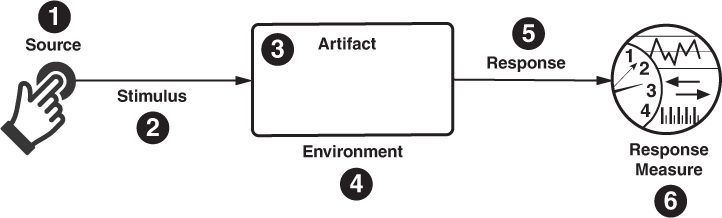
\includegraphics{Figures/qualityattributescenario.jpg}}
\caption{\label{Figure::The parts of a quality attribute scenario} The parts of a quality attribute scenario.}
\end{figure}
\index{Non-functional requirements}\index{testable}\index{unambiguous}\index{Source of stimulus}\index{Stimulus}\index{Environment}\index{Response}\index{Response measure}\index{uptime}\index{error rate}\index{Scenario}
\section{List of Significant Quality Attribute Scenarios\label{Section::SignificantQAS}}
\subsection{Availability\label{subSection::AvailabilityQA}}
\begin{enumerate}
    \item Source of stimulus: A user requests to stitch two images together.
    \item Stimulus: The user clicks on a button to start the stitching process.
    \item Artifact: The two images that the user wants to stitch together.
    \item Environment: The OpenCV Image Stitcher module is running on a computer.
    \item Response: The Image Stitcher module stitches the two images together and displays the result.
    \item Response measure:
    \begin{itemize}
        \item The response measure is the time it takes to stitch the two images together.
        \item The percentage of time that the library is able to process requests and return results without any errors or downtime.
        \item This can be measured using metrics such as uptime, response time, and error rate.
    \end{itemize}
\end{enumerate}
\begin{figure}[H]
\centering
\scalebox{0.6}{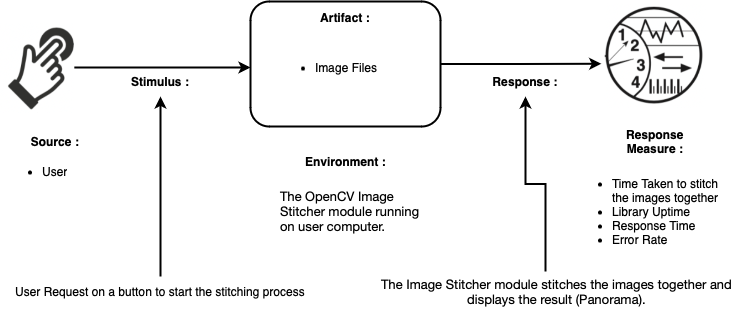
\includegraphics{Figures/Availability.png}}
\caption{\label{Figure::Quality Attribute Scenario for Availability} Quality Attribute Scenario for Availability \cite{drawio}.}
\end{figure}
A high availability score indicates that OpenCV is able to handle a large volume of requests and provide reliable results to users, ensuring that the application is always available and responsive.
In this scenario, the availability quality attribute is met if the Image Stitcher module is able to stitch the two images together in a timely manner. If the Image Stitcher module is not able to stitch the images together, or if it takes a long time to do so, then the availability quality attribute is not met.
\subsection{Deployability\label{subSection::DeployabilityQA}}
\begin{enumerate}
    \item Source of stimulus: A software developer wants to deploy the OpenCV Image Stitcher module in a new application.
    \item Stimulus: The developer downloads the OpenCV Image Stitcher module from the OpenCV website.
    \item Artifact: The OpenCV Image Stitcher module is a C++ library.
    \item Environment: The developer's development environment must have a C++ compiler and the OpenCV libraries installed.
    \item Response: The developer compiles the OpenCV Image Stitcher module and links it to their application.
    \item Response measure: The response measure is the time it takes to deploy the OpenCV Image Stitcher module in the new application.
\end{enumerate} 
\index{Deployability}\index{Energy Efficiency}\index{Integrability}\index{Modifiability}\index{Performance}
\begin{figure}[H]
\centering
\scalebox{0.6}{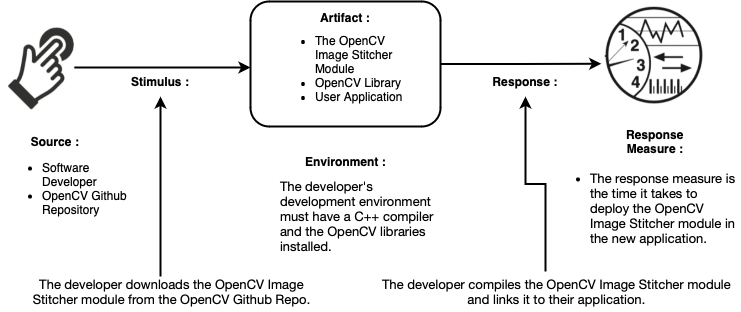
\includegraphics{Figures/Deployability.png}}
\caption{\label{Figure::Quality Attribute Scenario for Deployability} Quality Attribute Scenario for Deployability.}
\end{figure}
In this scenario, the deployability quality attribute is met if the OpenCV Image Stitcher module can be deployed in the new application in a timely manner. If the OpenCV Image Stitcher module cannot be deployed, or if it takes a long time to do so, then the deployability quality attribute is not met.
\subsection{Energy Efficiency\label{subSection::EnergyEfficiencyQA}}
\begin{enumerate}
    \item Source of stimulus: A user wants to use the OpenCV Image Stitcher module to stitch two images together on a mobile device.
    \item Stimulus: The user opens the application that uses the OpenCV Image Stitcher module.
    \item Artifact: The two images that the user wants to stitch together.
    \item Environment: The mobile device has a limited battery life.
    \item Response: The OpenCV Image Stitcher module stitches the two images together and displays the result.
    \item Response measure: The response measure is the amount of energy consumed by the mobile device while the OpenCV Image Stitcher module is running.
\end{enumerate}
\begin{figure}[H]
\centering
\scalebox{0.6}{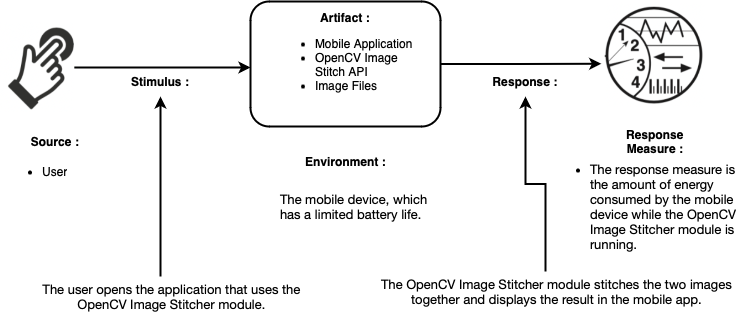
\includegraphics{Figures/energyefficiency.png}}
\caption{\label{Figure::Quality Attribute Scenario for Energy Efficiency} Quality Attribute Scenario for Energy Efficiency.}
\end{figure}
In this scenario, the energy efficiency quality attribute is met if the OpenCV Image Stitcher module is able to stitch the two images together while consuming as little energy as possible. If the OpenCV Image Stitcher module consumes a lot of energy, then the battery life of the mobile device will be reduced.
\subsection{Integrability\label{subSection::IntegrabilityQA}}
\begin{enumerate}
    \item Source of stimulus: Development team
    \item Stimulus: The development team needs to integrate openCV with a new software component.
    \item Artifact: openCV software package, new component
    \item Environment: Development environment with the new software component and its associated hardware and software.
    \item Response: The openCV software package is successfully integrated with the new software component and is fully functional.
    \item Response Measure: The development team measures the time it takes to integrate openCV with the new software component, the number of errors encountered during integration, and the ease of using openCV with the new software component.
\end{enumerate}
\begin{figure}[H]
\centering
\scalebox{0.5}{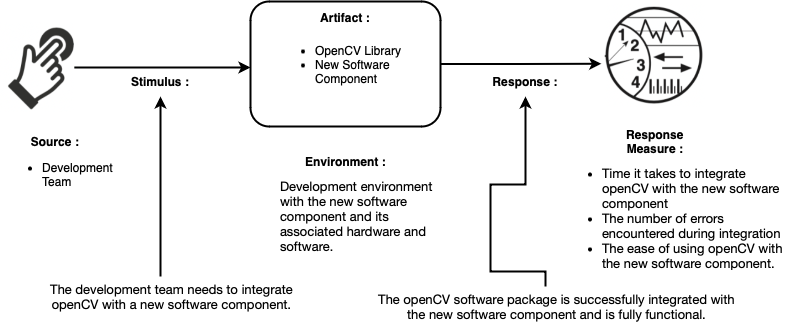
\includegraphics{Figures/Integratability.png}}
\caption{\label{Figure::Quality Attribute Scenario for Integrability} Quality Attribute Scenario for Integrability.}
\end{figure}
Additionally, the team may also measure the impact of the integration on the performance of the new software component and the overall system. The goal is to minimize integration time, errors, and impact on performance, while maximizing ease of use and compatibility with the new software component.
\subsection{Modifiability\label{subSection::ModifiabilityQA}}
\begin{enumerate}
    \item Source of stimulus: Product owner
    \item Stimulus: The product owner requests a new feature to be added to openCV.
    \item Artifact: openCV software package, new feature
    \item Environment: Development environment with the necessary hardware and software.
    \item Response: The development team modifies the openCV software package to include the new feature and ensures that it is fully functional.
    \item Response measure: The development team measures the time it takes to modify openCV to include the new feature, the number of errors encountered during modification, and the impact of the modification on the performance of openCV.
\end{enumerate}
\begin{figure}[H]
\centering
\scalebox{0.5}{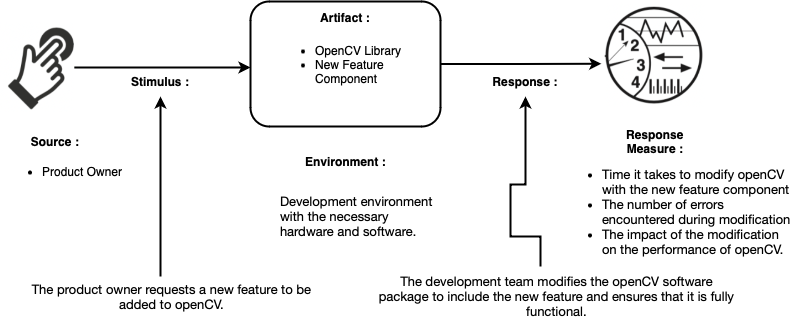
\includegraphics{Figures/modifiability.png}}
\caption{\label{Figure::Quality Attribute Scenario for Modifiability} Quality Attribute Scenario for Modifiability.}
\end{figure}
Additionally, the team may also measure the ease of maintaining the modified code and the impact of the modification on the overall system. The goal is to minimize modification time, errors, and impact on performance, while maximizing ease of maintenance and compatibility with the overall system.
\subsection{Performance\label{subSection::PerformanceQA}}
\begin{enumerate}
    \item Source of stimulus: User
    \item Stimulus: The user requests openCV to process a large image dataset.
    \item Artifact: openCV software package, image dataset, image library
    \item Environment: Production environment with the necessary hardware and software.
    \item Response: openCV processes the large image dataset within an acceptable time frame and with minimal errors.
    \item Response measure: The user measures the time it takes for openCV to process the large image dataset, the number of errors encountered during processing, and the resource utilization of the system during processing.
\end{enumerate}
\begin{figure}[H]
\centering
\scalebox{0.6}{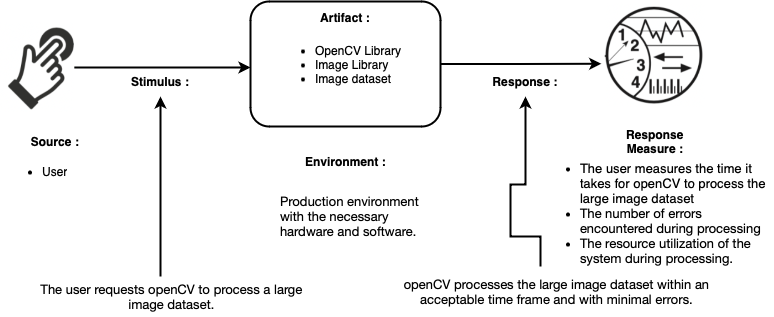
\includegraphics{Figures/Performance.png}}
\caption{\label{Figure::Quality Attribute Scenario for Performance} Quality Attribute Scenario for Performance.}
\end{figure}
Additionally, the user may also measure the accuracy of the processing results and the ease of integrating openCV with other software components in the production environment. The goal is to minimize processing time, errors, and resource utilization, while maximizing accuracy and ease of integration with other software components.
\subsection{Safety\label{subSection::SafetyQA}}
\begin{enumerate}
    \item Source of stimulus: Self-driving car system.
    \item Stimulus: The self-driving car system requests openCV to detect objects on the road and make decisions based on the detected objects.
    \item Artifact: openCV software package, car camera.
    \item Environment: Production environment in a self-driving car with the necessary hardware and software.
    \item Response: openCV accurately detects objects on the road and provides the self-driving car system with the necessary information to make safe driving decisions.
    \item Response measure: The self-driving car system measures the accuracy of openCV's object detection on the road, the number of false positives or false negatives encountered, and the impact of openCV's operation on the safety of the passengers and other vehicles on the road.
\end{enumerate}
\index{Safety}\index{Security}\index{Testability}\index{Usability}
\begin{figure}[H]
\centering
\scalebox{0.6}{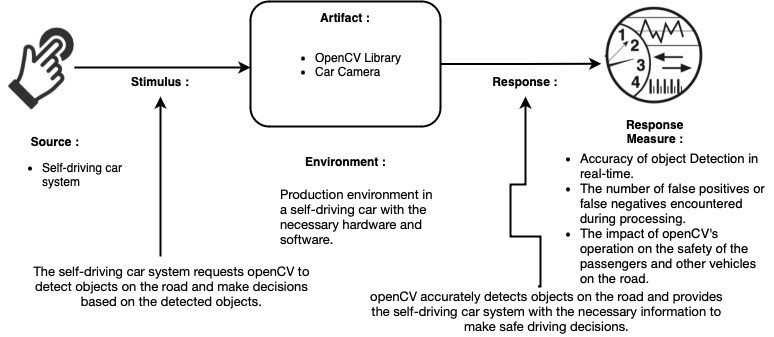
\includegraphics{Figures/Safety.png}}
\caption{\label{Figure::Quality Attribute Scenario for Safety} Quality Attribute Scenario for Safety.}
\end{figure}
Additionally, the system may also measure the ease of integrating openCV with other safety systems in the self-driving car. The goal is to maximize the accuracy of object detection while minimizing any safety hazards or risks associated with openCV's operation in the self-driving car.
\subsection{Security\label{subSection::SecurityQA}}
\begin{enumerate}
    \item Source of stimulus: Unauthorized user
    \item Stimulus: The unauthorized user attempts to gain access to sensitive information or disrupt the operation of openCV.
    \item Artifact: openCV software package, Security log report
    \item Environment: Production environment with the necessary hardware and software.
    \item Response: openCV detects and prevents the unauthorized user's attempts to gain access to sensitive information or disrupt the system's operation and does not compromise the security of the system or any sensitive information.
    \item Response measure: The system measures the number of successful and unsuccessful attempts by the unauthorized user to gain access to sensitive information or disrupt the system's operation, the impact of the unauthorized user's attempts on the security of the system and any sensitive information, and the effectiveness of openCV's security measures in preventing the unauthorized user's attempts.
\end{enumerate}
\begin{figure}[H]
\centering
\scalebox{0.5}{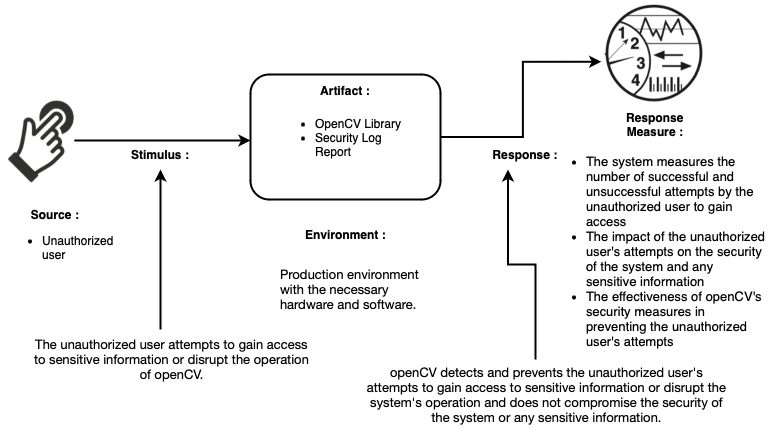
\includegraphics{Figures/Security.png}}
\caption{\label{Figure::Quality Attribute Scenario for Security} Quality Attribute Scenario for Security.}
\end{figure}
Additionally, the system may also measure the ease of maintaining and updating openCV's security measures to address any new vulnerabilities or threats. The goal is to minimize the number of successful unauthorized access attempts and their impact on the security of the system and any sensitive information.
\subsection{Testability\label{subSection::TestabilityQA}}
\begin{enumerate}
    \item Source of stimulus: Testing team
    \item Stimulus: The testing team needs to test the accuracy and performance of the openCV Image Stitching module in a real-world scenario.
    \item Artifact: openCV Image Stitching module, Image files
    \item Environment: Real-world environment with the necessary hardware and software on tester's computer.
    \item Response: The openCV Image Stitching module accurately stitches images in the real-world scenario and performs within acceptable performance parameters.
    \item Response measure: The testing team measures the accuracy of the openCV Image Stitching module in stitching images in the real-world scenario, the number of errors encountered during stitching, and the performance of the module in terms of processing time and resource utilization. Test-cases pass percentage for unique scenarios. Test Coverage percentage of openCV Image Stitching module.
\end{enumerate}
\begin{figure}[H]
\centering
\scalebox{0.5}{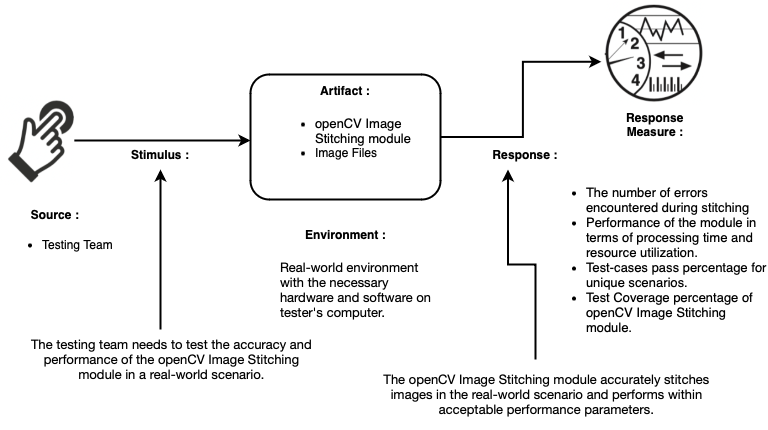
\includegraphics{Figures/Testability.png}}
\caption{\label{Figure::Quality Attribute Scenario for Testability} Quality Attribute Scenario for Testability.}
\end{figure}
Additionally, the team may also measure the ease of testing the openCV Image Stitching module in the real-world scenario and the effectiveness of any testing tools or frameworks used. The goal is to maximize the accuracy and performance of the openCV Image Stitching module in the real-world scenario while minimizing any testing time and effort required.
\subsection{Usability\label{subSection::UsabilityQA}}
\begin{enumerate}
    \item Source of stimulus: User
    \item Stimulus: The user needs to use openCV to perform image processing tasks.
    \item Artifact: openCV software package, image files
    \item Environment: User's environment with the necessary hardware and software.
    \item Response: The user is able to use openCV to perform image processing tasks with ease and efficiency.
    \item Response measure: The user measures the ease of learning and using openCV to perform image processing tasks, the time it takes to complete the tasks, and the user satisfaction with the user interface and overall usability of openCV.
\end{enumerate}
\begin{figure}[H]
\scalebox{0.5}{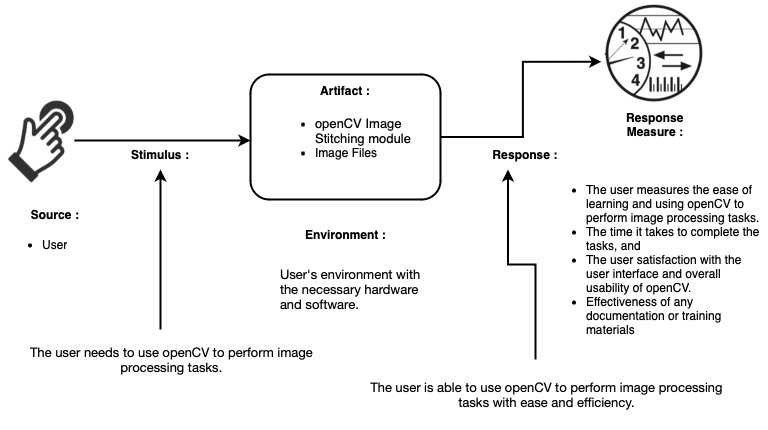
\includegraphics{Figures/Usability.png}}
\caption{\label{Figure::Quality Attribute Scenario for Usability} Quality Attribute Scenario for Usability.}
\end{figure}
Additionally, the user may also measure the effectiveness of any documentation or training materials provided with openCV. The goal is to maximize the ease of use and efficiency of openCV for image processing tasks, while minimizing the time and effort required to learn and use the software.
\section{Evaluation of Business risk and Architectural Significance\label{Section::QAratings}}
\begin{longtable}{|l|c|c|}
\hline
\textbf{Quality Attribute} & \textbf{Business Value (a)} & \textbf{Effect on Architecture (b)} \\
\hline
Availability & H & M \\
Deployability & M & M \\
Energy Efficiency & L & M \\
Integrability & M & M \\
Modifiability & H & M \\
Performance & H & H \\
Safety & H & H \\
Security & H & H \\
Testability & H & M \\
Usability & M & M \\
\hline
\caption{Quality Attribute Evaluation \label{Table::Quality Attribute Evaluation}}
\end{longtable}
\newpage
\subsection{Understanding the values}
Grading Scale Used:\newline
\newline
\underline{\textbf{Rating:}} (a, b):\newline
\textbf{a:} the ASR’s\index{ASR!Architecturally significant requirement} business value\index{Business Value}(importance)\newline
\textbf{b:} the effect on the architecture(difficulty)\newline
\\
\underline{\textbf{Key:}}\newline
\textbf{H}=high\newline
\textbf{M}=medium\newline
\textbf{L}=low\newline
\begin{enumerate}
    \item Availability: openCV is a mature library with a large community of users and developers. There are many different ways to install and use openCV, which makes it easy to deploy in a variety of environments. This is why we rated availability as high.
    \item Deployability: openCV is available for a variety of platforms, including Windows, Linux, and macOS. There are also many different ways to deploy openCV, such as as a static library, a shared library, or a Docker image. This is why we rated deployability as medium.
    \item Energy Efficiency: openCV uses a variety of techniques to optimize its performance, such as using hardware acceleration and image compression. This is why we rated energy efficiency as low.
    \item Integrability: openCV provides a variety of APIs, such as C++, Python, and Java, which make it easy to integrate with other languages and frameworks. This is why we rated integrabilty as medium.
    \item Modifiability: openCV is a open source library, which means that the source code is available for anyone to modify. This makes it easy to customize openCV to meet the specific needs of a project. This is why we rated modifiability as high.
    \item Performance: openCV is designed to be fast and efficient, even on resource-constrained devices. This is why we rated performance as high.
    \item Safety: openCV is designed to be secure and reliable, even in critical applications. This is why I rated safety as high.
    \item Security: openCV is designed to be resistant to attack and intrusion. This is why we rated security as high.
    \item Testability: openCV provides a variety of tools and resources to help developers test their code. This makes it easy to ensure that openCV is working properly before it is deployed in production. This is why we rated testability as high.
    \item Usability: openCV provides a variety of documentation and tutorials to help developers get started. This makes it easy for anyone to use openCV, regardless of their experience level. This is why we rated usability as medium.
\end{enumerate}
\section{Utiltity Tree\label{Section::utilityTree}}
\subsection{Introduction}
\paragraph{} A utility tree starts with the root node "Utility" representing the overall "goodness" of the system. Major Quality Attributes (QAs) are listed under the root node. Each QA is then further refined with specific aspects relevant to the system. These refinements can be broken down into specific Quality Attribute Scenarios (ASRs).
\paragraph{} ASRs are placed as leaves on the tree and evaluated based on business value and technical risk. Business value is assessed as high, medium, or low, indicating the importance of meeting the requirement. Technical risk is evaluated as high, medium, or low, reflecting the level of concern and confidence in meeting the ASR.
\paragraph{} In summary, a utility tree outlines the system's QAs, their refinements, and ASRs as scenarios. These scenarios are then evaluated based on business value and technical risk.
\subsection{Tabular form of Utility Tree}
\begin{figure}[H]
\centering
\scalebox{0.55}{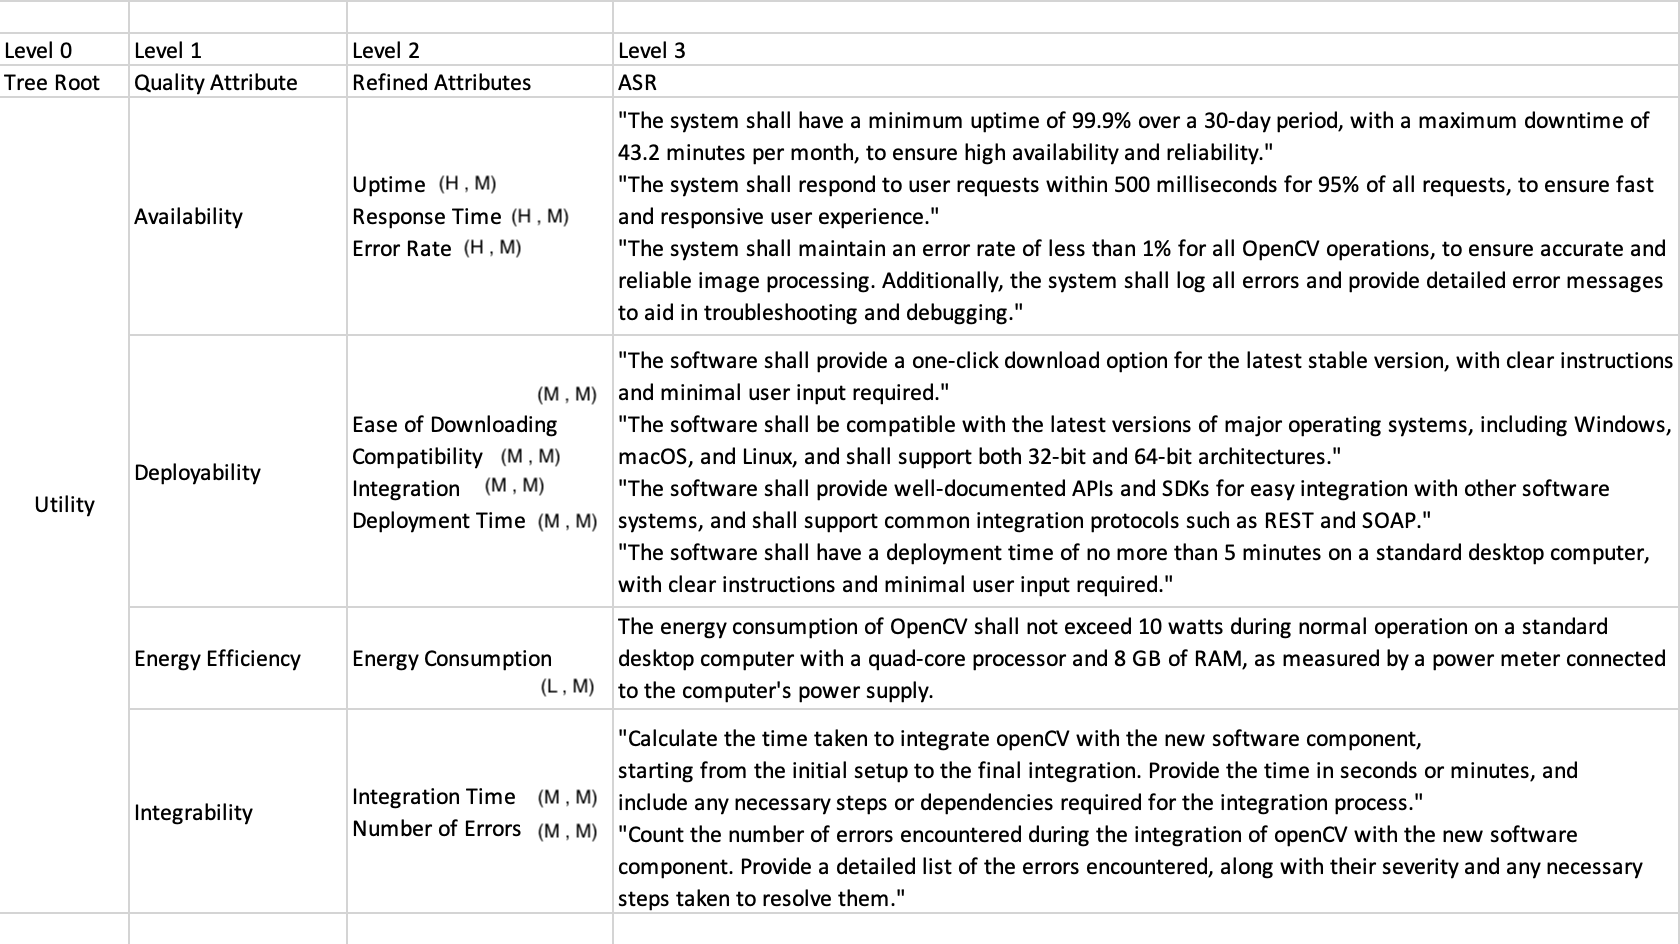
\includegraphics{Figures/UtilityTree1.png}}
\caption{\label{Figure::UtilityTree1} Utility Tree - 1.}
\end{figure}
\begin{figure}[H]
\centering
\scalebox{0.5}{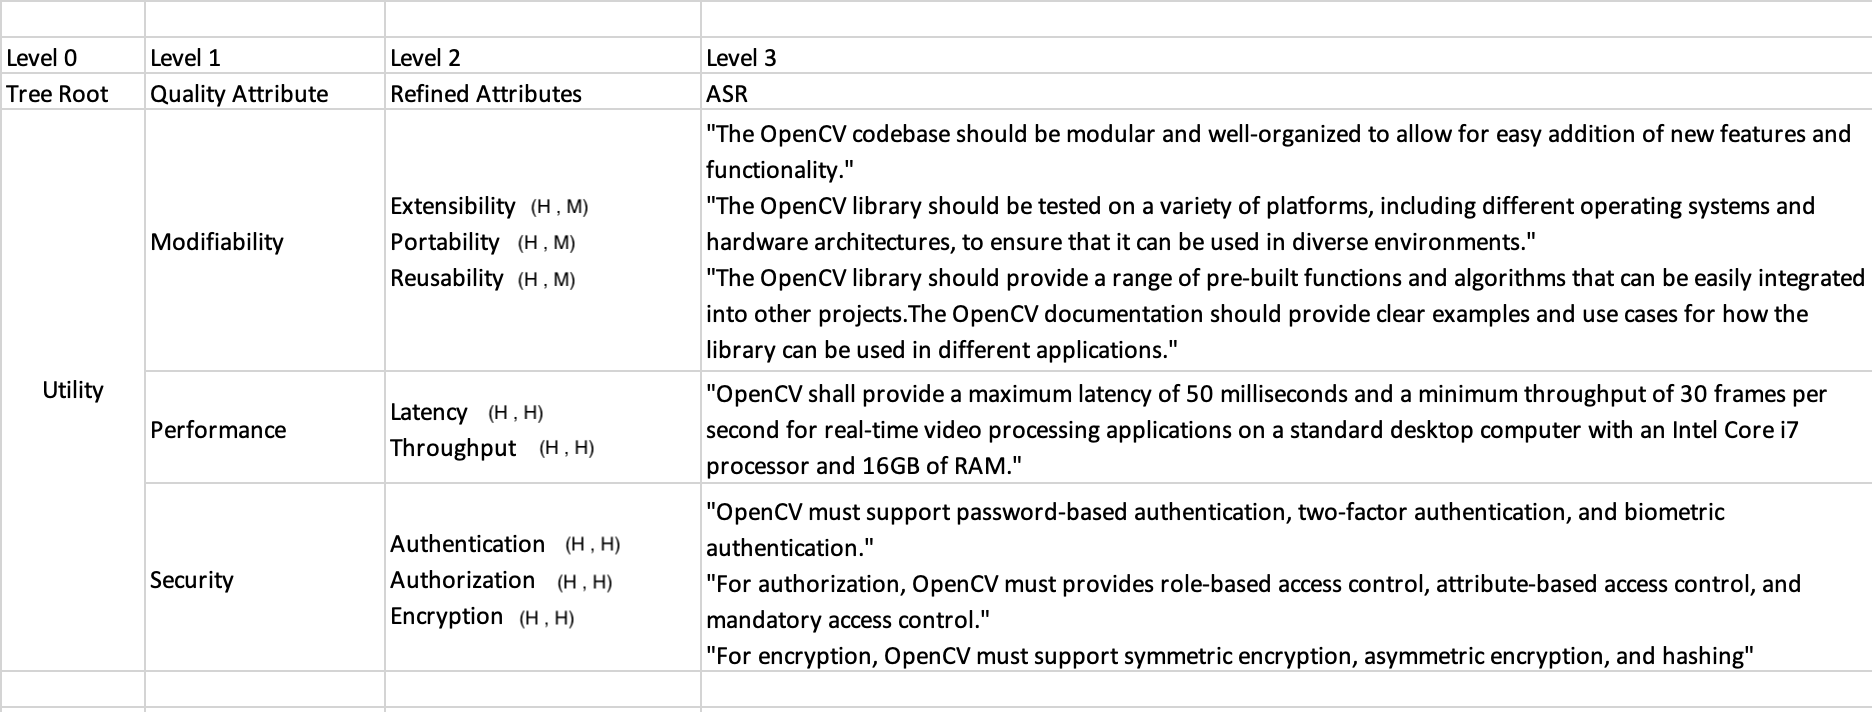
\includegraphics{Figures/UtilityTree2.png}}
\caption{\label{Figure::UtilityTree2} Utility Tree - 2.}
\end{figure}
\begin{figure}[H]
\centering
\scalebox{0.5}{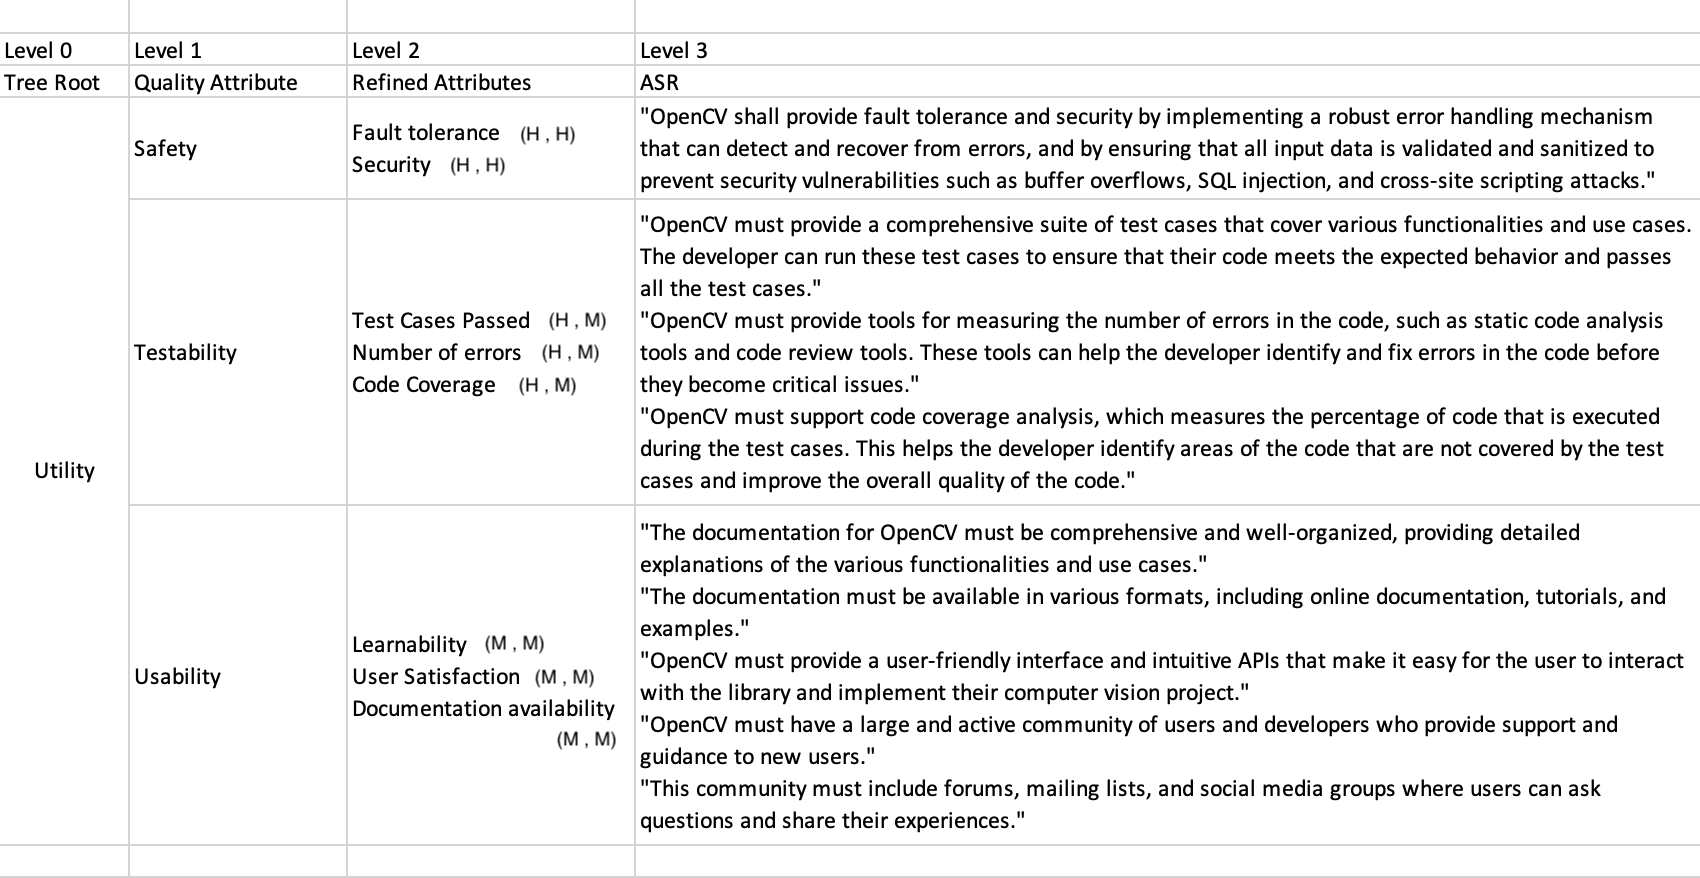
\includegraphics{Figures/UtilityTree3.png}}
\caption{\label{Figure::UtilityTree3} Utility Tree - 3.}
\end{figure}
\chapter{Risks\\
\small{\textit{-- Nikhil Kumar G, Raj Palival}}
\index{Chapter!Risks}
\index{Risks}
\label{Chapter::Risks}}

\section{Introduction \label{Section::RisksChapterIntro}}
OpenCV, like any software, is not immune to risks and challenges. While it is a powerful and widely-used open-source computer vision library, it's important to recognize that there may be potential pitfalls that can impact its usage and effectiveness. These risks can manifest in various areas, such as functionality, performance, security, compatibility, and documentation. Understanding these risks allows developers to be proactive in addressing them and ensuring the smooth integration and deployment of OpenCV in their applications. By staying informed, keeping up with updates, seeking community support, and following best practices, developers can mitigate these risks and harness the full potential of OpenCV for their computer vision needs.

\section{Risks \label{Section::Risks}}
Based on observations and investigations, there are a few anticipated risks and areas that can be improved in OpenCV:

\subsection{Security Risks \label{subSection::SecurityRisk}}
\begin{enumerate}
     \item OpenCV may be vulnerable to security attacks such as buffer overflows or injection attacks, which can lead to unauthorized access or control of systems.
     \item Malicious users could exploit vulnerabilities in the library, potentially causing damage or compromising sensitive data.     
 \end{enumerate}

\subsubsection{Tactics for Security Risks \label{subsubSection::SecurityTactic}}
The tactics that can be applied to above risks are:
\begin{itemize}
    \item Regularly update OpenCV to the latest version to incorporate security patches and fixes.
    \item Implement secure coding practices when using OpenCV, such as input validation and proper memory management.
    \item Perform security audits and vulnerability assessments to identify and mitigate potential risks.
    \item Encourage the OpenCV community to report and address security issues promptly.
\end{itemize}
\index{pitfalls}\index{manifest}\index{Security Risks}\index{Tactics}\index{memory management}
\subsection{Performance Risks \label{subSection::PerformanceRisk}}
\begin{enumerate}
     \item OpenCV may face performance limitations, especially when processing large-scale or real-time video streams or when working with resource-intensive algorithms.
     \item Inefficient use of system resources or suboptimal algorithms could result in slow execution or inadequate responsiveness.    
 \end{enumerate}

 \subsubsection{Tactics for Performance Risks \label{subsubSection::PerformanceTactic}}
The tactics that can be applied to above risks are:
\begin{itemize}
    \item Optimize algorithms and data structures to enhance computational efficiency.
    \item Leverage hardware acceleration technologies like GPU (Graphics Processing Unit) or dedicated AI accelerators when applicable.
    \item Employ parallel processing techniques, such as multi-threading or distributed computing, to distribute computational load and improve performance.
    \item Continuously benchmark and profile OpenCV applications to identify bottlenecks and areas for optimization.
\end{itemize}

\subsection{Usability Risks \label{subSection::UsabilityRisk}}
\begin{enumerate}
     \item OpenCV has a steep learning curve for newcomers and may be challenging for developers without a strong background in computer vision.
     \item Documentation may be insufficient or not beginner-friendly, making it difficult to understand and utilize the library effectively.   
 \end{enumerate}

 \subsubsection{Tactics for Usability Risks \label{subsubSection::UsabilityTactic}}
The tactics that can be applied to above risks are:
\begin{itemize}
    \item Enhance the official OpenCV documentation with comprehensive and well-structured tutorials, examples, and explanations.
    \item Foster an active community that provides support, answers questions, and shares best practices.
    \item Develop user-friendly APIs and higher-level abstractions to simplify common computer vision tasks.
    \item Provide educational resources, such as online courses or workshops, to help developers acquire the necessary skills to use OpenCV effectively.
\end{itemize}
\index{Performance Risks}\index{suboptimal algorithms}\index{resource-intensive algorithms}\index{Usability Risks}\index{computational load} \index{multi-threading} \index{distributed computing}
\subsection{Compatibility and Portability Risks \label{subSection::CompatibilityRisk}}
\begin{enumerate}
     \item OpenCV may face compatibility issues with different operating systems, hardware architectures, or versions of dependencies.
     \item Lack of portability can limit the usage of OpenCV in diverse environments or on specific platforms.  
 \end{enumerate}

 \subsubsection{Tactics for Compatibility and Portability Risks \label{subsubSection::CompatibilityTactic}}
The tactics that can be applied to above risks are:
\begin{itemize}
     \item Conduct extensive testing on different platforms and environments to identify and resolve compatibility issues.
     \item Follow best practices for cross-platform development and ensure proper handling of platform-specific features or dependencies.
     \item Provide pre-compiled binaries or packages for popular operating systems to simplify installation and deployment.
     \item Encourage community contributions and feedback to address compatibility issues specific to certain environments.
\end{itemize}

\subsection{Documentation Risks \label{subSection::DocumentationRisk}}
\begin{enumerate}
     \item OpenCV's documentation may lack clarity, completeness, or up-to-date information, leading to confusion and difficulties for developers.
     \item Inadequate learning resources can make it challenging for beginners to grasp the concepts and effectively utilize the library. 
 \end{enumerate}

 \subsubsection{Tactics for Documentation Risks \label{subsubSection::DocumentationTactic}}
The tactics that can be applied to above risks are:
\begin{itemize}
     \item Establish clear and well-structured documentation that covers all aspects of OpenCV, including detailed explanations, API references, and usage examples.
     \item Maintain an active and accessible community forum or support channel to address questions and provide guidance.
     \item Collaborate with educational institutions or organizations to develop comprehensive learning resources, tutorials, and courses for OpenCV.
     \item Encourage community contributions to enhance documentation and create additional learning materials.
\end{itemize}
\index{Portability Risks}\index{Documentation Risks}\index{Accuracy}\index{Robustness Risks}\index{datasets}
\subsection{Accuracy and Robustness Risks \label{subSection::RobustnessRisk}}
\begin{enumerate}
     \item OpenCV's computer vision algorithms may exhibit inaccuracies or lack robustness in certain scenarios or edge cases.
     \item Performance degradation or incorrect results can occur when the algorithms fail to handle specific image variations or conditions. 
 \end{enumerate}

 \subsubsection{Tactics for Accuracy and Robustness Risks \label{subsubSection::RobustnessTactic}}
The tactics that can be applied to above risks are:
\begin{itemize}
     \item Continuously evaluate and benchmark the performance and accuracy of OpenCV algorithms across a wide range of test cases and datasets.
     \item Collect and analyze user feedback and reported issues to identify areas where algorithms need improvement.
     \item Encourage collaboration and contributions from the computer vision research community to refine and enhance existing algorithms.
     \item Maintain a well-organized repository of sample images and datasets to facilitate testing and evaluation of algorithmic performance.
\end{itemize}
\index{Scalability}\index{Concurrency Risks}\index{Intel TBB}\index{OpenMP}\index{Privacy Risk}
\subsection{Scalability and Concurrency Risks \label{subSection::ScalabilityRisk}}
\begin{enumerate}
     \item OpenCV may encounter challenges in scaling and efficiently utilizing multiple processing cores or distributed computing resources.
     \item In scenarios where high concurrency is required, such as real-time video processing or large-scale computer vision pipelines, performance bottlenecks or resource contention can arise.
 \end{enumerate}

 \subsubsection{Tactics for Scalability and Concurrency Risks \label{subsubSection::ScalabilityTactic}}
The tactics that can be applied to above risks are:
\begin{itemize}
     \item Implement parallel processing techniques, such as multi-threading or task-based concurrency, to distribute workloads and maximize resource utilization.
     \item Utilize frameworks or libraries that offer higher-level concurrency abstractions, such as OpenMP or Intel TBB, to simplify parallel programming in OpenCV.
     \item Optimize critical sections of code and minimize thread synchronization overhead to improve scalability and reduce contention.
     \item Explore distributed computing frameworks, such as Apache Spark or Hadoop, for processing large-scale computer vision tasks across multiple machines.
\end{itemize}

\subsection{Data Privacy Risks \label{subSection::PrivacyRisk}}
\begin{enumerate}
     \item OpenCV applications may process and analyze sensitive data, such as images containing personally identifiable information or proprietary content.
     \item Inadequate data privacy measures can lead to privacy breaches or unauthorized access to confidential information.
 \end{enumerate}

 \subsubsection{Tactics for Data Privacy Risks \label{subsubSection::PrivacyTactic}}
The tactics that can be applied to above risks are:
\begin{itemize}
     \item Adhere to relevant data privacy regulations and standards, such as GDPR or HIPAA, when handling sensitive data with OpenCV.
     \item Implement data anonymization techniques to remove or obfuscate personally identifiable information from images or other data inputs.
     \item Employ encryption mechanisms to protect data at rest or in transit during OpenCV processing.
     \item Educate developers on best practices for data privacy and encourage the use of secure coding principles when working with OpenCV.
\end{itemize}

\subsection{Community Engagement Risks \label{subSection::CommunityRisk}}
\begin{enumerate}
     \item OpenCV may face challenges in actively engaging the community and effectively incorporating user feedback and contributions.
     \item Limited community involvement can result in slower resolution of issues, missed opportunities for improvement, and reduced adoption.
 \end{enumerate}

 \subsubsection{Tactics for Community Engagement Risks \label{subsubSection::CommunityTactic}}
The tactics that can be applied to above risks are:
\begin{itemize}
     \item Foster an inclusive and collaborative community environment where users feel encouraged to provide feedback, report issues, and contribute to the development of OpenCV.
     \item Establish transparent communication channels, such as mailing lists, forums, or dedicated feedback platforms, to gather and address user input effectively.
     \item Regularly acknowledge and appreciate community contributions through recognition, documentation credits, or code attribution.
     \item Actively participate in computer vision conferences, workshops, and hackathons to engage with the broader community and promote OpenCV's advancements.
\end{itemize}

\subsection{Integration Risks \label{subSection::IntegrationRisk}}
\begin{enumerate}
     \item OpenCV's integration with machine learning frameworks and libraries may face challenges in terms of compatibility, ease of use, or performance.
     \item Inadequate integration can hinder the adoption of state-of-the-art machine learning techniques within OpenCV applications.
 \end{enumerate}
\index{Integration Risks}
 \subsubsection{Tactics for Integration Risks \label{subsubSection::IntegrationTactic}}
The tactics that can be applied to above risks are:
\begin{itemize}
     \item Establish seamless integration with popular machine learning frameworks, such as TensorFlow or PyTorch, by providing dedicated APIs or interoperability layers.
     \item Offer pre-trained models or model conversion tools that enable users to easily leverage deep learning models within OpenCV.
     \item Collaborate with the machine learning community to identify and address integration issues, ensure compatibility, and keep up with the latest advancements in the field.
     \item Provide extensive documentation and examples showcasing the integration of OpenCV with machine learning, covering common use cases and best practices.
\end{itemize}


\chapter{Architecture\\
\small{\textit{-- Nikhil Kumar G, Raj Palival}}
\index{Chapter!Architecture}
\index{Architecture}
\label{Chapter::Architecture}}

\section{Description\label{Section::ArchitectureIntro}}
OpenCV (Open Source Computer Vision Library \cite{OCV}) is an open-source library that includes several hundreds of computer vision algorithms. It has a modular structure architecture, which means that the package includes several modules with shared or static libraries. 

\section{Modules \label{subSection::ModulesList}}
There are two types of modules available:
\begin{enumerate}
     \item Main Modules: These modules are the core components of the OpenCV library that provide essential computer vision functionalities.
     \item Extra modules: These are additional modules that offer extended features and algorithms not included in the main modules.
 \end{enumerate}
Below is a list of all the modules available in each category:

\subsection{Main Modules\label{subSection::MainModules}}
\begin{enumerate}
     \item core. Core functionality: a compact module defining basic data structures, including the dense multi-dimensional array Mat and basic functions used by all other modules. \index{Core functionality}
     \item imgproc. Image Processing: an image processing module that includes linear and non-linear image filtering, geometrical image transformations (resize, affine and perspective warping, generic table-based remapping), color space conversion, histograms, and so on. \index{Image Processing}
     \item imgcodecs. Image file reading and writing: This module in OpenCV provides functions for reading and writing image files in various formats \index{imgcodecs}
     \item videoio. Video I/O: This module in OpenCV provides functions for reading and writing video files and accessing video streams from cameras or other devices. \index{videoio}
     \item highgui. High-level GUI: This module in OpenCV provides high-level functions for creating graphical user interfaces (GUI) to display and interact with images, videos, and other visual data. \index{High-level GUI}
     \item video. Video Analysis: This module in OpenCV involves performing various operations on video frames, such as object detection, tracking, motion analysis, and frame manipulation. \index{object detection}
     \item calib3d. Camera Calibration and 3D Reconstruction: This module in OpenCV provides functions for camera calibration and 3D reconstruction. \index{Camera Calibration}
     \item features2d. 2D Features Framework: This module in OpenCV provides a framework for detecting and describing 2D image features. These features can be used for tasks such as image matching, object recognition, and image stitching. \index{2D Features Framework}
     \item objdetect. Object Detection: This module in OpenCV provides functions and pre-trained models for object detection. It allows you to detect and localize objects within images or video frames.\index{objdetect}
     \item dnn. Deep Neural Network module: This module in OpenCV provides a flexible and efficient framework for working with deep neural networks (DNNs). It allows you to load pre-trained models, perform inference on images or videos, and fine-tune models. \index{Deep Neural Network}
     \item ml. Machine Learning: This module in OpenCV provides a set of machine learning algorithms and tools for various tasks, including classification, regression, clustering, and dimensionality reduction.\index{Machine Learning}
     \item flann. Clustering and Search in Multi-Dimensional Spaces: This module in OpenCV provides efficient algorithms for clustering and searching in multi-dimensional spaces. FLANN stands for Fast Library for Approximate Nearest Neighbors. \index{Clustering}
     \item photo. Computational Photography: This module refers to the use of computational techniques and algorithms to enhance or modify digital photographs.\index{Computational Photography} 
     \item stitching. Images stitching: Image stitching is the process of combining multiple overlapping images to create a larger, seamless panorama. \index{Images stitching}
     \item gapi. Graph API: This module is a computational graph-based framework provided by OpenCV that allows for efficient parallel execution of image processing and computer vision algorithms. \index{Graph API}
 \end{enumerate}
 \subsection{Extra Modules\label{subSection::ExtraModules}}
\begin{enumerate}
     \item alphamat. Alpha Matting \index{Alpha Matting}
     \item aruco. Aruco markers, module functionality was moved to objdetect module \index{Aruco markers}
     \item barcode. Barcode detecting and decoding methods \index{Barcode detecting}
     \item bgsegm. Improved Background-Foreground Segmentation Methods \index{Segmentation}
     \item bioinspired. Biologically inspired vision models and derivated tools \index{bioinspired}
     \item ccalib. Custom Calibration Pattern for 3D reconstruction
     \item cudaarithm. Operations on Matrices
     \item cudabgsegm. Background Segmentation
     \item cudacodec. Video Encoding/Decoding
     \item cudafeatures2d. Feature Detection and Description
     \item cudafilters. Image Filtering
     \item cudaimgproc. Image Processing
     \item cudalegacy. Legacy support
     \item cudaobjdetect. Object Detection
     \item cudaoptflow. Optical Flow
     \item cudastereo. Stereo Correspondence
     \item cudawarping. Image Warping
     \item cudev. Device layer
     \item cvv. GUI for Interactive Visual Debugging of Computer Vision Programs
     \item datasets. Framework for working with different datasets
     \item dnn objdetect. DNN used for object detection
     \item dnn superres. DNN used for super resolution
     \item dpm. Deformable Part-based Models
     \item face. Face Analysis
     \item freetype. Drawing UTF-8 strings with freetype/harfbuzz
     \item fuzzy. Image processing based on fuzzy mathematics
     \item hdf. Hierarchical Data Format I/O routines
     \item hfs. Hierarchical Feature Selection for Efficient Image Segmentation
     \item img hash. The module brings implementations of different image hashing algorithms.
     \item intensity transform. The module brings implementations of intensity transformation algorithms to adjust image contrast.
     \item julia. Julia bindings for OpenCV
     \item line descriptor. Binary descriptors for lines extracted from an image
     \item mcc. Macbeth Chart module
     \item optflow. Optical Flow Algorithms
     \item ovis. OGRE 3D Visualiser
     \item phase unwrapping. Phase Unwrapping API
     \item plot. Plot function for Mat data
     \item quality. Image Quality Analysis (IQA) API
     \item rapid. silhouette based 3D object tracking
     \item reg. Image Registration
     \item rgbd. RGB-Depth Processing
     \item saliency. Saliency API
     \item sfm. Structure From Motion
     \item shape. Shape Distance and Matching
     \item stereo. Stereo Correspondance Algorithms
     \item structured light. Structured Light API
     \item superres. Super Resolution
     \item surface matching. Surface Matching
     \item text. Scene Text Detection and Recognition
     \item tracking. Tracking API
     \item videostab. Video Stabilization
     \item viz. 3D Visualizer
     \item wechat qrcode. WeChat QR code detector for detecting and parsing QR code.
     \item xfeatures2d. Extra 2D Features Framework
     \item ximgproc. Extended Image Processing
     \item xobjdetect. Extended object detection
     \item xphoto. Additional photo processing algorithms
\end{enumerate}

\section{Grouping Modules\label{Section::GroupingModules}}
The modules don't have a clear order or hierarchy. Core, python, and java are commonly used modules, but there isn't a definite separation between them. Often, a module that uses the core module also depends on another module, which makes the structure very complex.\\\\
However, we can group all the modules in three categories:
\begin{enumerate}
     \item Main Functionality
     \item Extended Functionality
     \item High Level GUI
\end{enumerate}

\section{15 Most Important Modules\label{Section::HighLevelView}}
Below is a figure of the 15 most important modules in the three categories discussed above:
\begin{figure}[H]
     \centering
     \scalebox{0.8}{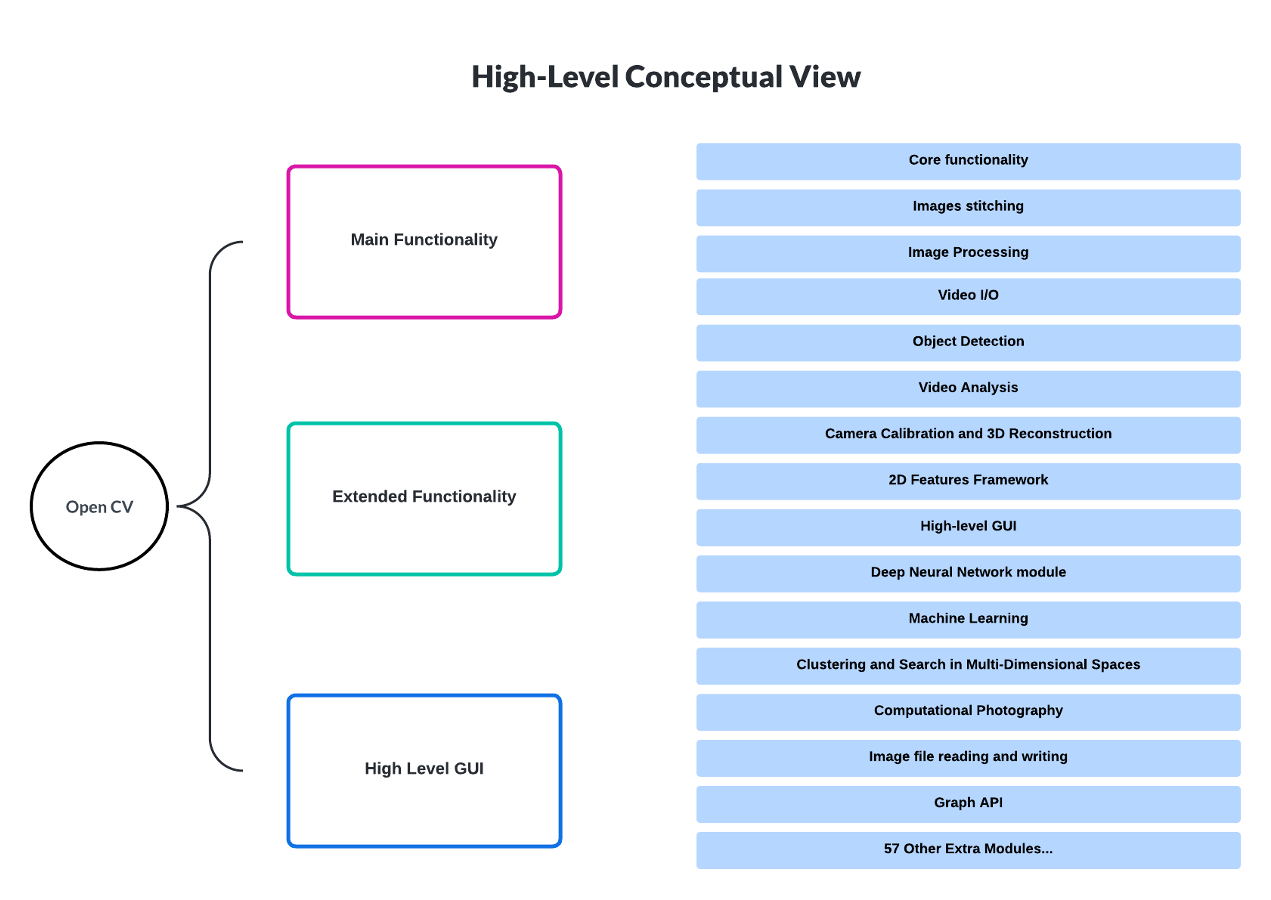
\includegraphics{Figures/Conceptualview.png}}
     \caption{\label{Figure::HighLevelView} High Level Conceptual View}
\end{figure}
\pagebreak

\section{4+1 View of Architecture\label{Section::4+1view}}
The 4+1 architectural view model provides multiple perspectives on the architecture of a system \cite{UNB}. Such as:
\begin{enumerate}
         \item Implementation View
         \item Use Case View
         \item Logical View
         \item Process View
         \item Deployment View
\end{enumerate}
We will use an example of one module to explain the rest of the OpenCV modules in OpenCV’s architecture. More on this later.
\subsection{Implementation View\label{subSection::ImplementationView}} \index{Implementation View}
The implementation view is an architectural view that  provides a detailed perspective on how the system is implemented and how the implementation artifacts are organized and interact with each other.\\\\
     In our case we will consider the following:
     \begin{itemize}
         \item Perspective: Developers, Proj. mngs.
         \item Stage: Design
         \item Focus: Subsystem decomposition
         \item Concerns: Software management
         \item Artefacts: Modules structure, Package diagram
     \end{itemize}
\subsubsection{Implementation View Artefacts\label{subsubSection::ImplementationView}} \index{Artefacts}
The modules structure below shows how all the modules in OpenCV interact with each other. It is clear that the modules in OpenCV are interconnected in a very complex way. \\\\

Modules Structure: Diagram taken from source \cite{OGB} 

\begin{figure}[H]
     \centering
     \scalebox{0.15}{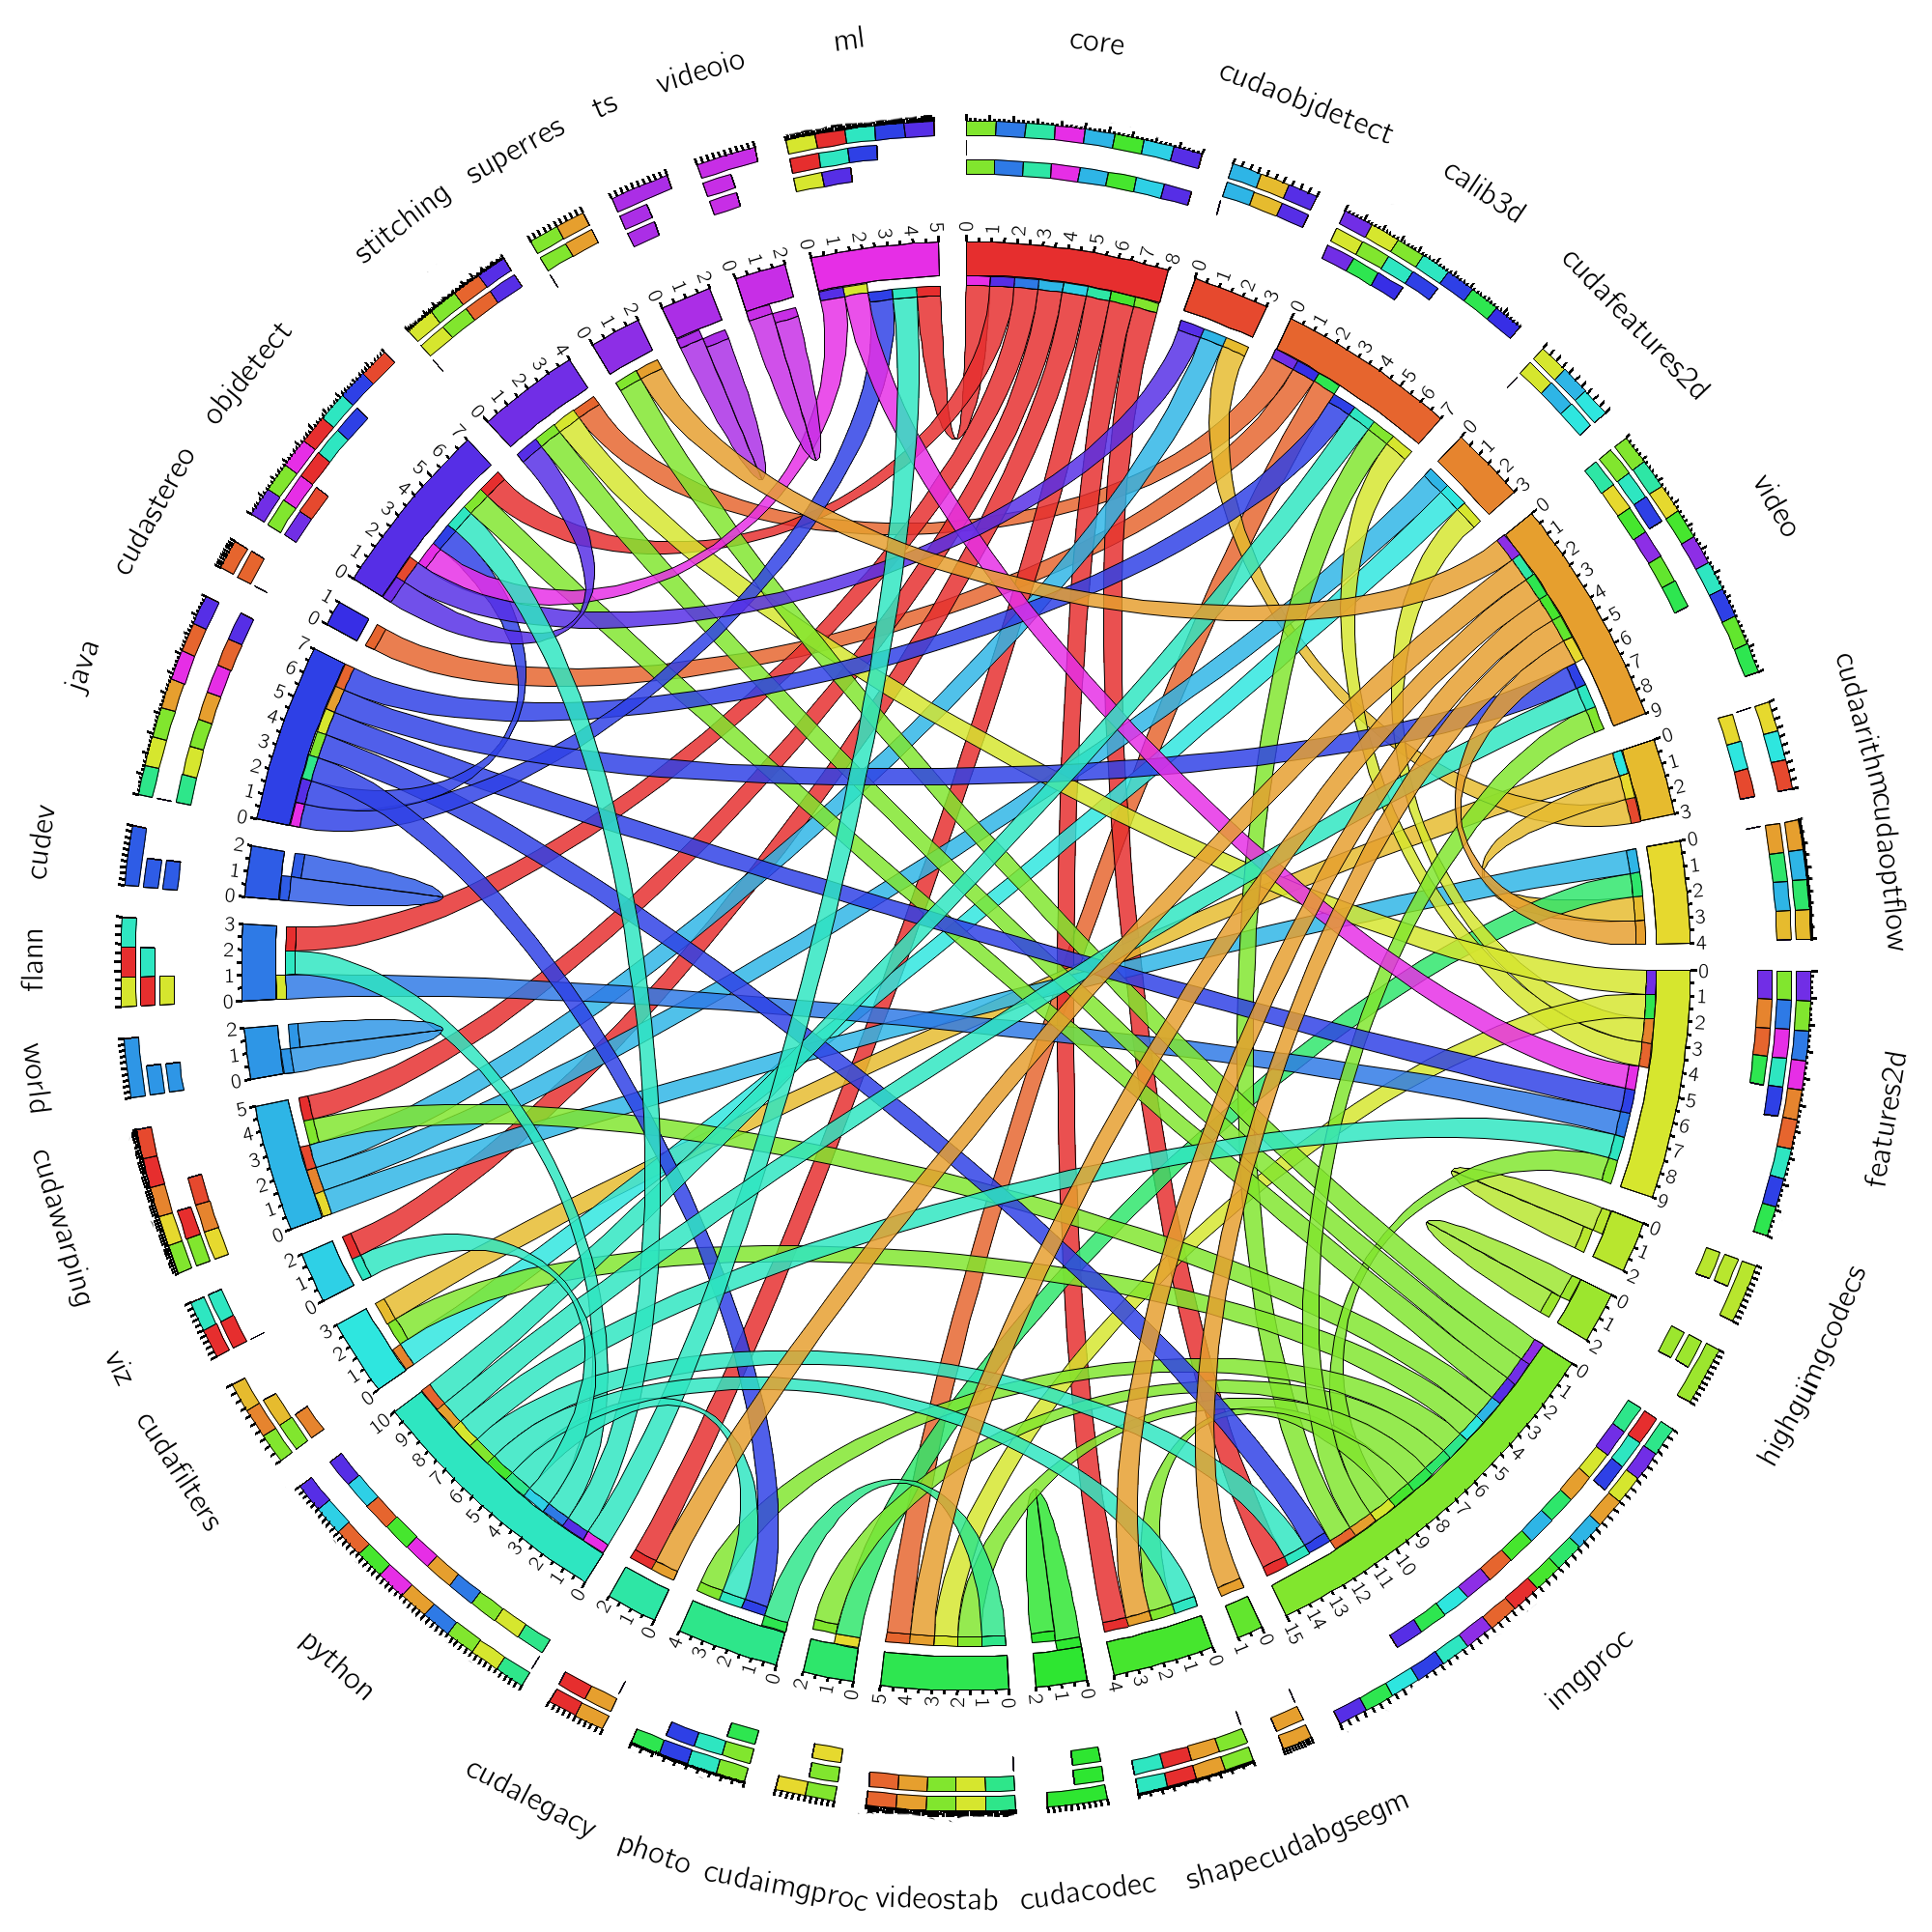
\includegraphics{Figures/ModulesStructure.png}}
     \caption{\label{Figure::ModulesStructure} Modules Interconnection Structure}
\end{figure}
Because of its complex nature, we will zoom into the architecture a little bit and understand one such important module of OpenCV among the 15 most important modules through all the 4+1 views' from here on:
\begin{itemize}
         \item Image Stitching Module (stitching.): Famously used to create panorama images \cite{6896208}. \index{panorama} 
\end{itemize}
The idea is to understand this one module which in-turn sort of explains the rest of the OpenCV modules in OpenCV's architecture. \\\\
Below is a Package Diagram of Image Stitching Module:\\\\
The diagram includes 3 levels:
\begin{enumerate}
         \item 1st Level: It is the OpenCV package that contains all modules.
         \item 2nd Level: It shows how the Image Stitching module is Interacting with other modules in OpenCV package.
         \item 3rd Level: Shows the functions present in Image Stitching module and the other two modules.
\end{enumerate}

\begin{figure}[H]
     \centering
     \scalebox{0.5}{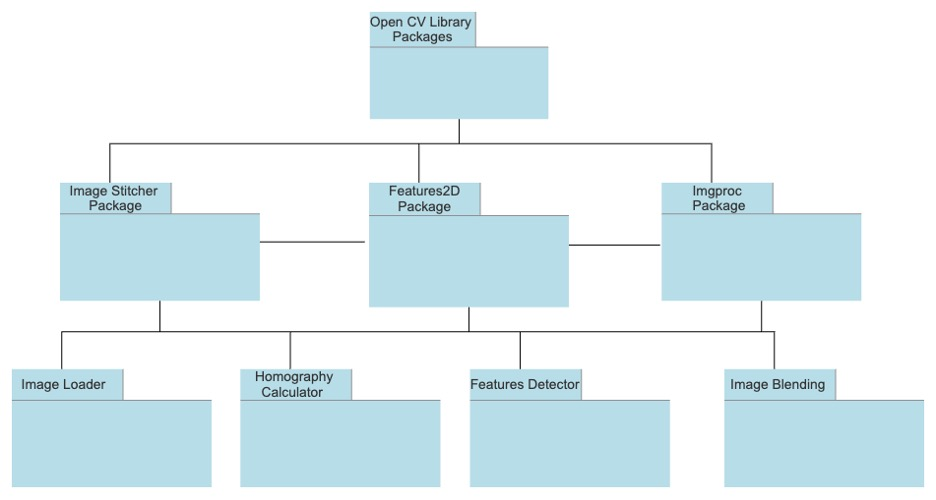
\includegraphics{Figures/PackageDiagram.jpg}}
     \caption{\label{Figure::ImageStitcherPackageDiagram
} Image Stitcher Package Diagram}
\end{figure}

\subsubsection{Functions\label{subsubSection::Functions}}
\begin{enumerate}
         \item Image Loader: It is used to load and prepare the images in Image Stitching package for stitching process.
         \item Homography Calculator: It is used to calculate a homography matrix between two sets of corresponding points in an image. \index{Homography}
         \item Features Detector: It is used to identify and extract distinctive features or points of interest from an image.
         \item Image Blending: It is the process of combining two or more images to create a single composite image that preserves the important information from each input image. \index{Image Blending}
\end{enumerate}
\pagebreak

\subsection{Use Case View\label{subSection::UserCaseView}} \index{User Case View}
The use case view is an architectural view that focuses on describing the system's functionality from the perspective of its users or external actors.\\\\
     In our case we will consider the following:
     \begin{itemize}
         \item Perspective: End users
         \item Stage: Putting it alltogether
         \item Concerns: Understandability, usability
         \item Focus: Feature decomposition
         \item Artefact: Use-case diagram
     \end{itemize}

\subsubsection{Use Case Diagram\label{subsubSection::UseCaseDiag}}
\begin{figure}[H]
     \centering
     \scalebox{0.68}{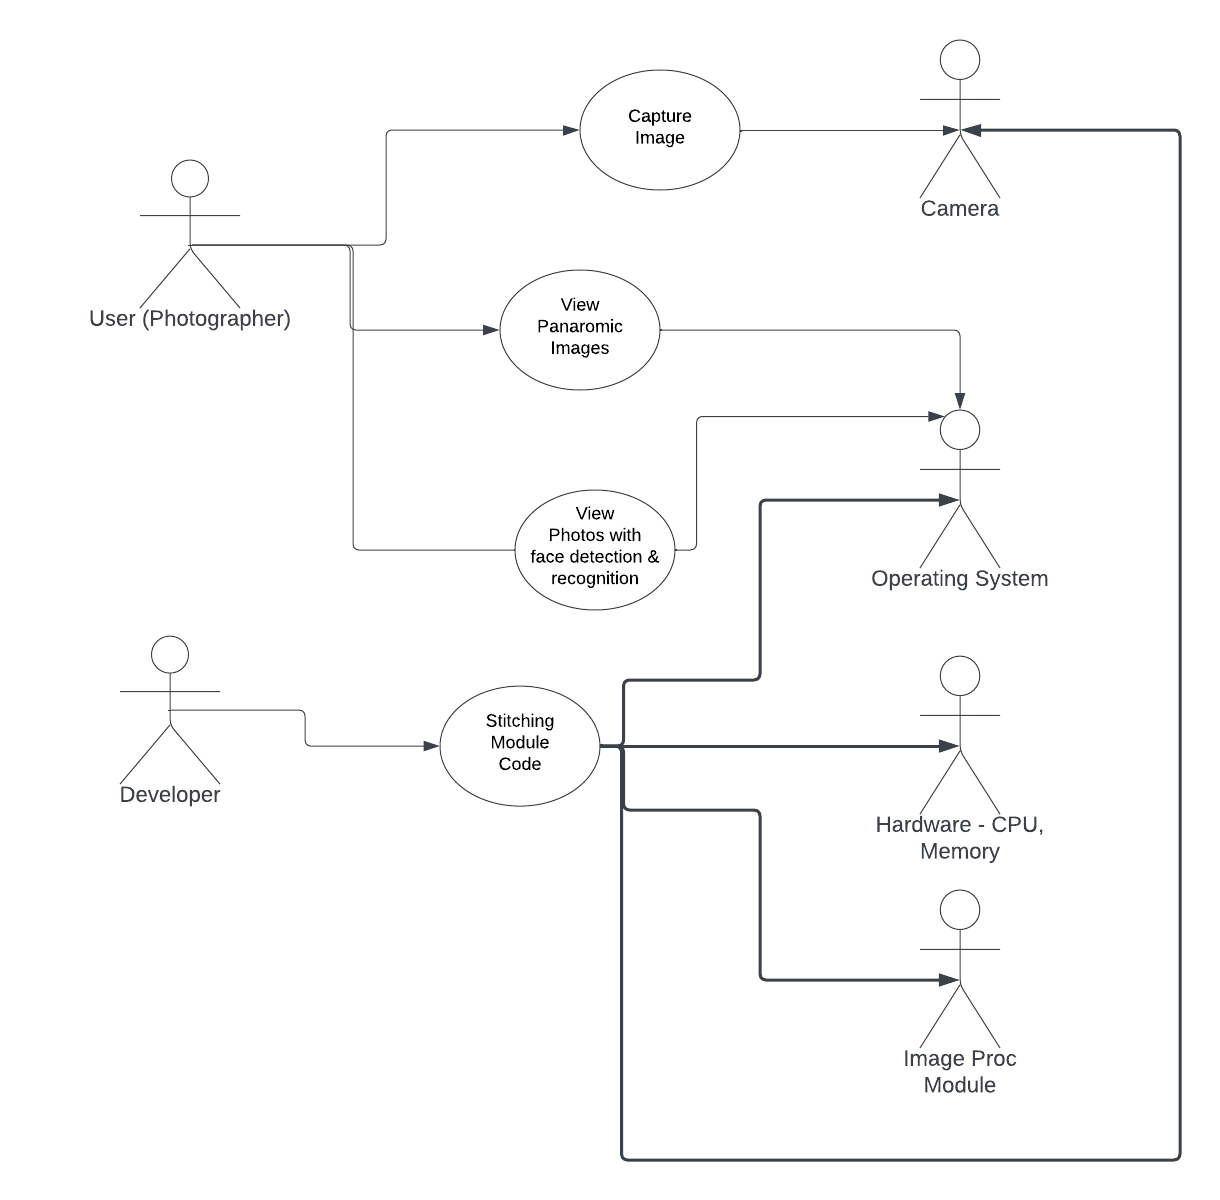
\includegraphics{Figures/Use Case Diagram of ImageStitchingModule.png}}
     \caption{\label{Figure::UseCaseDiagram
} Use Case Diagram for Image Stiching Module \cite{lucidchart}}
\end{figure}

We have the following in our diagram:
\begin{enumerate}
         \item Actors: Two actors \index{Actors}
         \begin{enumerate}
         \item User: Photographer has 3 use cases:- \index{Photographer}
             \begin{enumerate}
             \item To capture images
             \item View panaromic images
             \item View photos with face detection and recognition.
             \end{enumerate}
         \item Developer has 1 use case:- \index{Developer}
             \begin{enumerate}
             \item Develop stitching module code
             \end{enumerate}
\end{enumerate}
         \item Use Cases: Four use cases 
         \begin{enumerate}
             \item To capture images
             \item View panaromic images
             \item View photos with face detection and recognition.
             \item Develop stitching module code
         \end{enumerate}

         \item External Actors: Four external actors
         \begin{enumerate}
             \item Camera: Facilitates in capturing images \index{Camera}
             \item Operating System: Used by both User and developer for their use cases \index{Operating System}
             \item Hardware Components: CPU, Memory \index{CPU} \index{Memory}
             \item Image Proc Module: Provides a wide range of functions and algorithms for manipulating and enhancing images.
         \end{enumerate}
         
\end{enumerate}


\pagebreak

\subsection{Logical View\label{subSection::LogicalView}} \index{Logical View}
The logical view is an architectural view that focuses on representing the high-level structure and organization of the system's functionality and behavior. It provides an abstraction of the system's functionality and its relationships, without delving into implementation details. \\\\
     In our case we will consider the following:
     \begin{itemize}
         \item Perspective: Analysts, Designers Stage: Requirement analysis \index{Analysts}
         \item Focus: Object oriented decomposition
         \item Concerns: Functionality
         \item Artefacts: Class diagram \cite{UMLdiagram}
     \end{itemize}

\begin{figure}[H]
     \centering
     \scalebox{0.6}{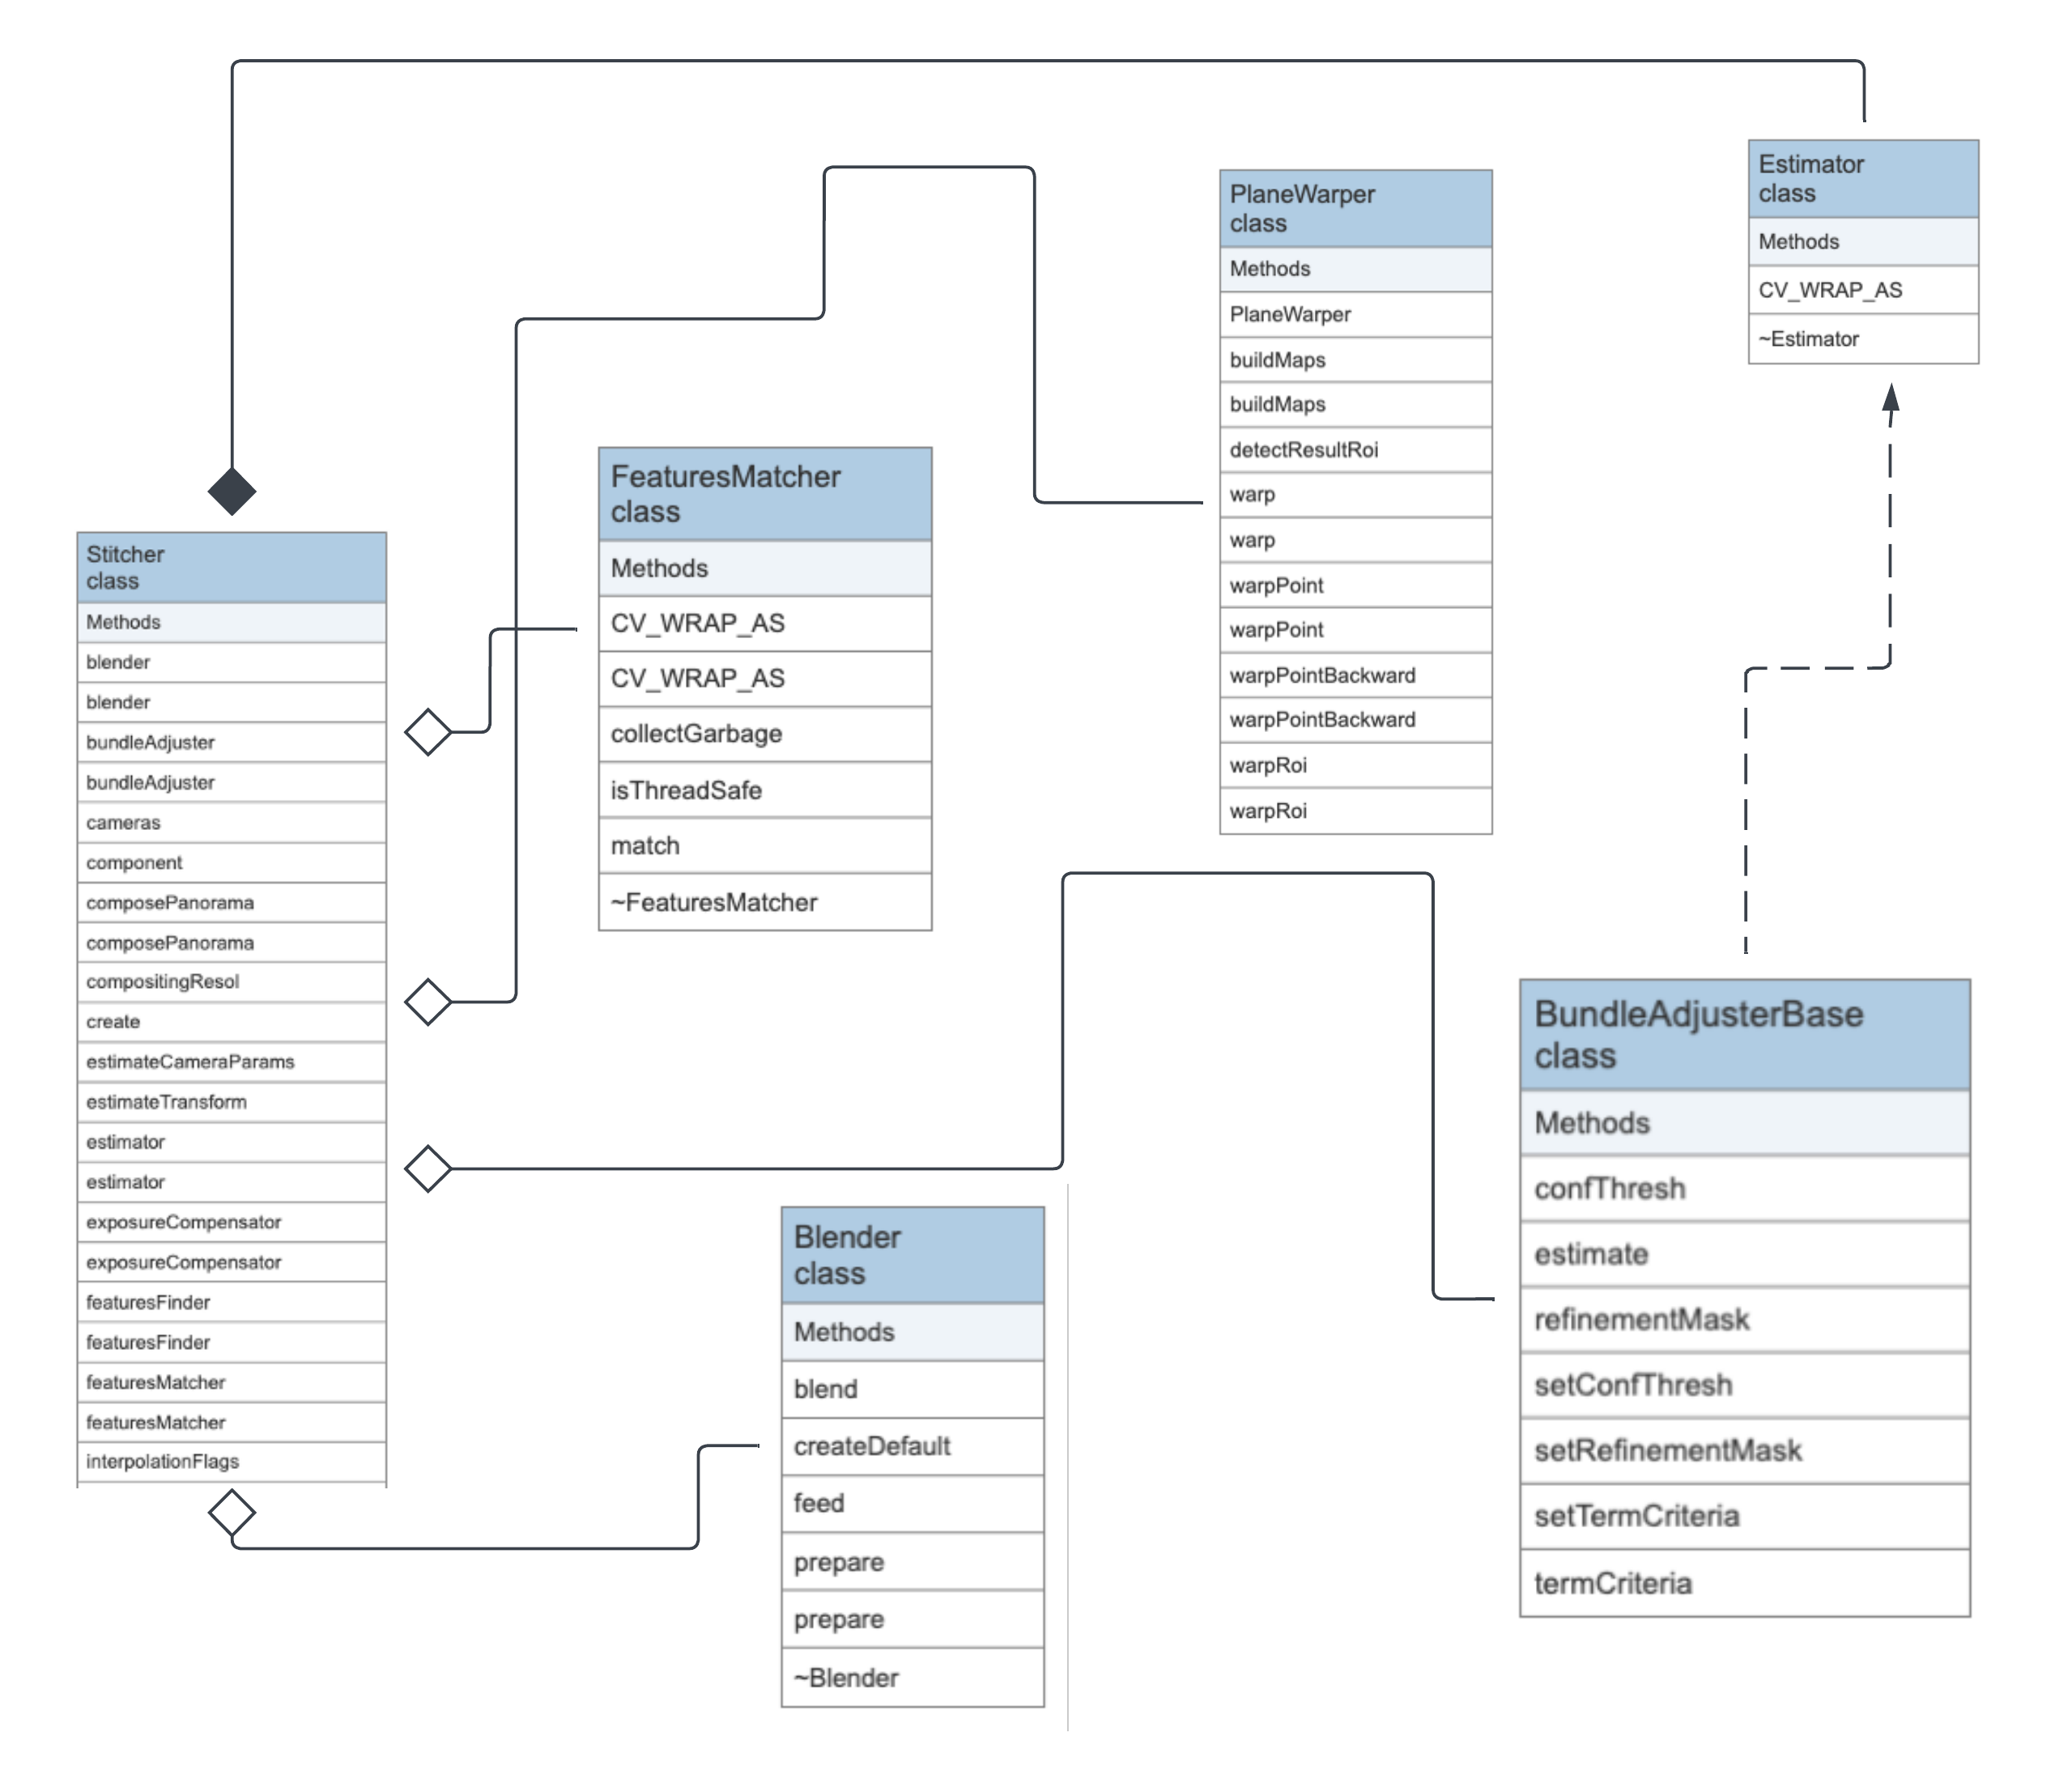
\includegraphics{Figures/ClassDiagram.png}}
     \caption{\label{Figure::BriefOverview} Class Diagram of Image Stitching Module \cite{smartdraw}}
\end{figure}
The logical view of OpenCV's Image Stitching module describes the system's functionality and the relationships between its components. The module consists of several classes, including the Stitcher class, Features Matcher class, Plane Warper class, Blender class, BundleAdjusterBaseClass, and Estimator class. Here is a brief description of each class and how they depend on each other:
\begin{enumerate}
    \item Stitcher class: The Stitcher class is the main class in the Image Stitching module. It provides the functionality to stitch multiple images together to create a panoramic image. The Stitcher class uses other classes in the module to perform various tasks, such as feature detection, feature matching, and image blending.
    \item Features Matcher class: The Features Matcher class is responsible for detecting and matching features in the input images. It uses various algorithms to detect and match features, such as the SIFT algorithm and the SURF algorithm.
    \item Plane Warper class: The Plane Warper class is responsible for warping the input images to a common plane. It uses various algorithms to perform the warping, such as the Homography algorithm and the Affine algorithm.
    \item Blender class: The Blender class is responsible for blending the warped images together to create a seamless panoramic image. It uses various algorithms to perform the blending, such as the Multi-band blending algorithm and the Feather blending algorithm.
    \item BundleAdjusterBaseClass: The BundleAdjusterBaseClass is responsible for adjusting the parameters of the stitching process to improve the quality of the output image. It uses various algorithms to adjust the parameters, such as the Levenberg-Marquardt algorithm and the Gauss-Newton algorithm.
    \item Estimator class: The Estimator class is responsible for estimating the camera parameters of the input images. It uses various algorithms to estimate the parameters, such as the RANSAC algorithm and the Least Squares algorithm.\\
\end{enumerate}
These classes depend on each other in a hierarchical manner. The Stitcher class is the main class that uses the other classes to perform various tasks. The Features Matcher class and the Estimator class are used by the Stitcher class to detect and match features and estimate camera parameters, respectively. The Plane Warper class is used by the Stitcher class to warp the input images to a common plane. The Blender class is used by the Stitcher class to blend the warped images together to create a seamless panoramic image. Finally, the BundleAdjusterBaseClass is used by the Stitcher class to adjust the parameters of the stitching process to improve the quality of the output image. Overall, these classes work together to provide the functionality of the Image Stitching module in OpenCV.
\pagebreak


\subsection{Process View\label{subSection::ProcessView}}
The process view is an architectural view that focuses on illustrating the runtime behavior and concurrency aspects of a system. It provides a perspective on how the system's functionality is executed and how different components or processes interact and collaborate during runtime.\\\\
     In our case we will consider the following:
     \begin{itemize}
         \item Perspective: System Integrators \index{System Integrators}
         \item Stage: Design
         \item Focus: Process decomposition
         \item Concerns: Performance, scalability, throughput \index{throughput}
         \item Artefacts: Sequence diagram \index{Sequence diagram}
     \end{itemize}
     
\subsubsection{Sequence Diagram\label{subsubSection::SequenceDiag}}
\begin{figure}[H]
     \centering
     \scalebox{0.38}{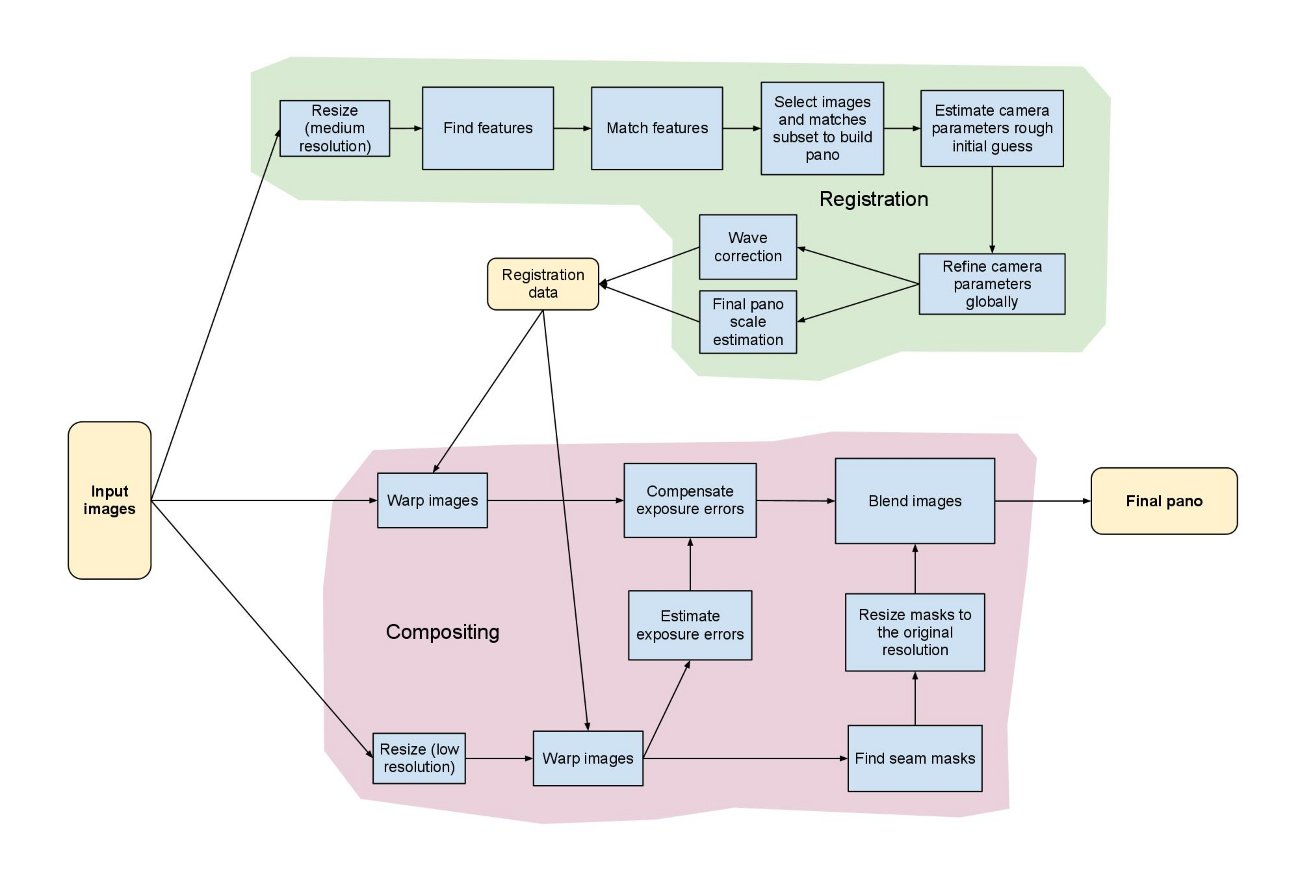
\includegraphics{Figures/StitchingPipeline.jpg}}
     \caption{\label{Figure::StitchingPipeline} Sequence Diagram of Image Stitching Module} \index{Stitching Pipeline}
\end{figure}
The process view of OpenCV's Image Stitching module describes the system's behavior and how it responds to external events. The module performs several operations to stitch multiple images together to create a panoramic image. Here is a brief description of each operation and the steps involved:
\begin{enumerate}
    \item Step 1 - Input Images:\\ The first operation is to input the images that need to be stitched together. These images are typically captured using a camera or downloaded from a source.

    \item Step 2 - Registration:\\ The second operation is registration, which involves several steps:
    \begin{itemize}
        \item Resize (medium resolution): The input images are resized to a medium resolution to reduce the computational complexity of the feature detection and matching algorithms.
        \item Find features: The feature detection algorithm is used to detect features in the input images, such as corners, edges, and blobs.
        \item Match features: The feature matching algorithm is used to match the features between the input images.
        \item Select images and matches subset to build panorama: The input images and their corresponding feature matches are selected to build the panorama.
        \item Estimate camera parameters rough initial guess: The camera parameters of the input images are estimated using a rough initial guess.
        \item Refine camera parameters globally: The camera parameters are refined globally using a bundle adjustment algorithm.
        \item Wave correction: The wave correction algorithm is used to correct the distortion caused by the camera lens.
        \item Final panorama scale estimation: The final scale of the panorama is estimated based on the camera parameters and the input images.
    \end{itemize}

    \item Step 3 - Registration data :\\ The registration data, including the camera parameters and the warped images, are passed to the compositing operation.

    \item Step 4 - Compositing:\\ The final operation is compositing, which involves several steps:
    \begin{itemize}
        \item Warp images: The warped images are transformed to a common coordinate system using the estimated camera parameters.
        \item Estimate exposure errors: The exposure errors in the input images are estimated using an exposure estimation algorithm.
        \item Compensate exposure errors: The exposure errors in the input images are compensated using an exposure compensation algorithm.
        \item Resize (low resolution): The final panoramic image is resized to a low resolution for display or storage purposes.
        \item Warp images: The warped images are transformed again to the original resolution.
        \item Find seam masks: The seam masks are found using a seam finding algorithm.
        \item Resize masks to original resolution: The seam masks are resized to the original resolution.
        \item Blend images: The blended image is created by blending the warped images together using a blending algorithm.
    \end{itemize}
    \item Step 5 - Final panorama:\\ The final panoramic image is created by combining the blended image and the seam masks.
\end{enumerate}
Overall, the process view of OpenCV's Image Stitching module describes the system's behavior and how it responds to external events, such as input images and user requests. The module performs several operations, including registration and compositing, to stitch multiple images together to create a beautiful panoramic image.
\pagebreak

\subsection{Deployment View\label{subSection::DeploymentView}}
The deployment view is an architectural view that focuses on illustrating how the software components of a system are deployed and distributed across hardware resources. It provides a representation of the physical infrastructure and deployment topology of the system.\\\\ \index{Deployment View}
     In our case we will consider the following:
     \begin{itemize}
         \item Perspective: System Engineers
         \item Stage: Design
         \item Focus: Map software to hardware
         \item Concerns: System topology, delivery, installation, communication
         \item Artefacts: Deployment diagram
     \end{itemize}

\subsubsection{Deployment Diagram\label{subsubSection::DeploymentDiag}}
\begin{figure}[H]
     \centering
     \scalebox{0.9}{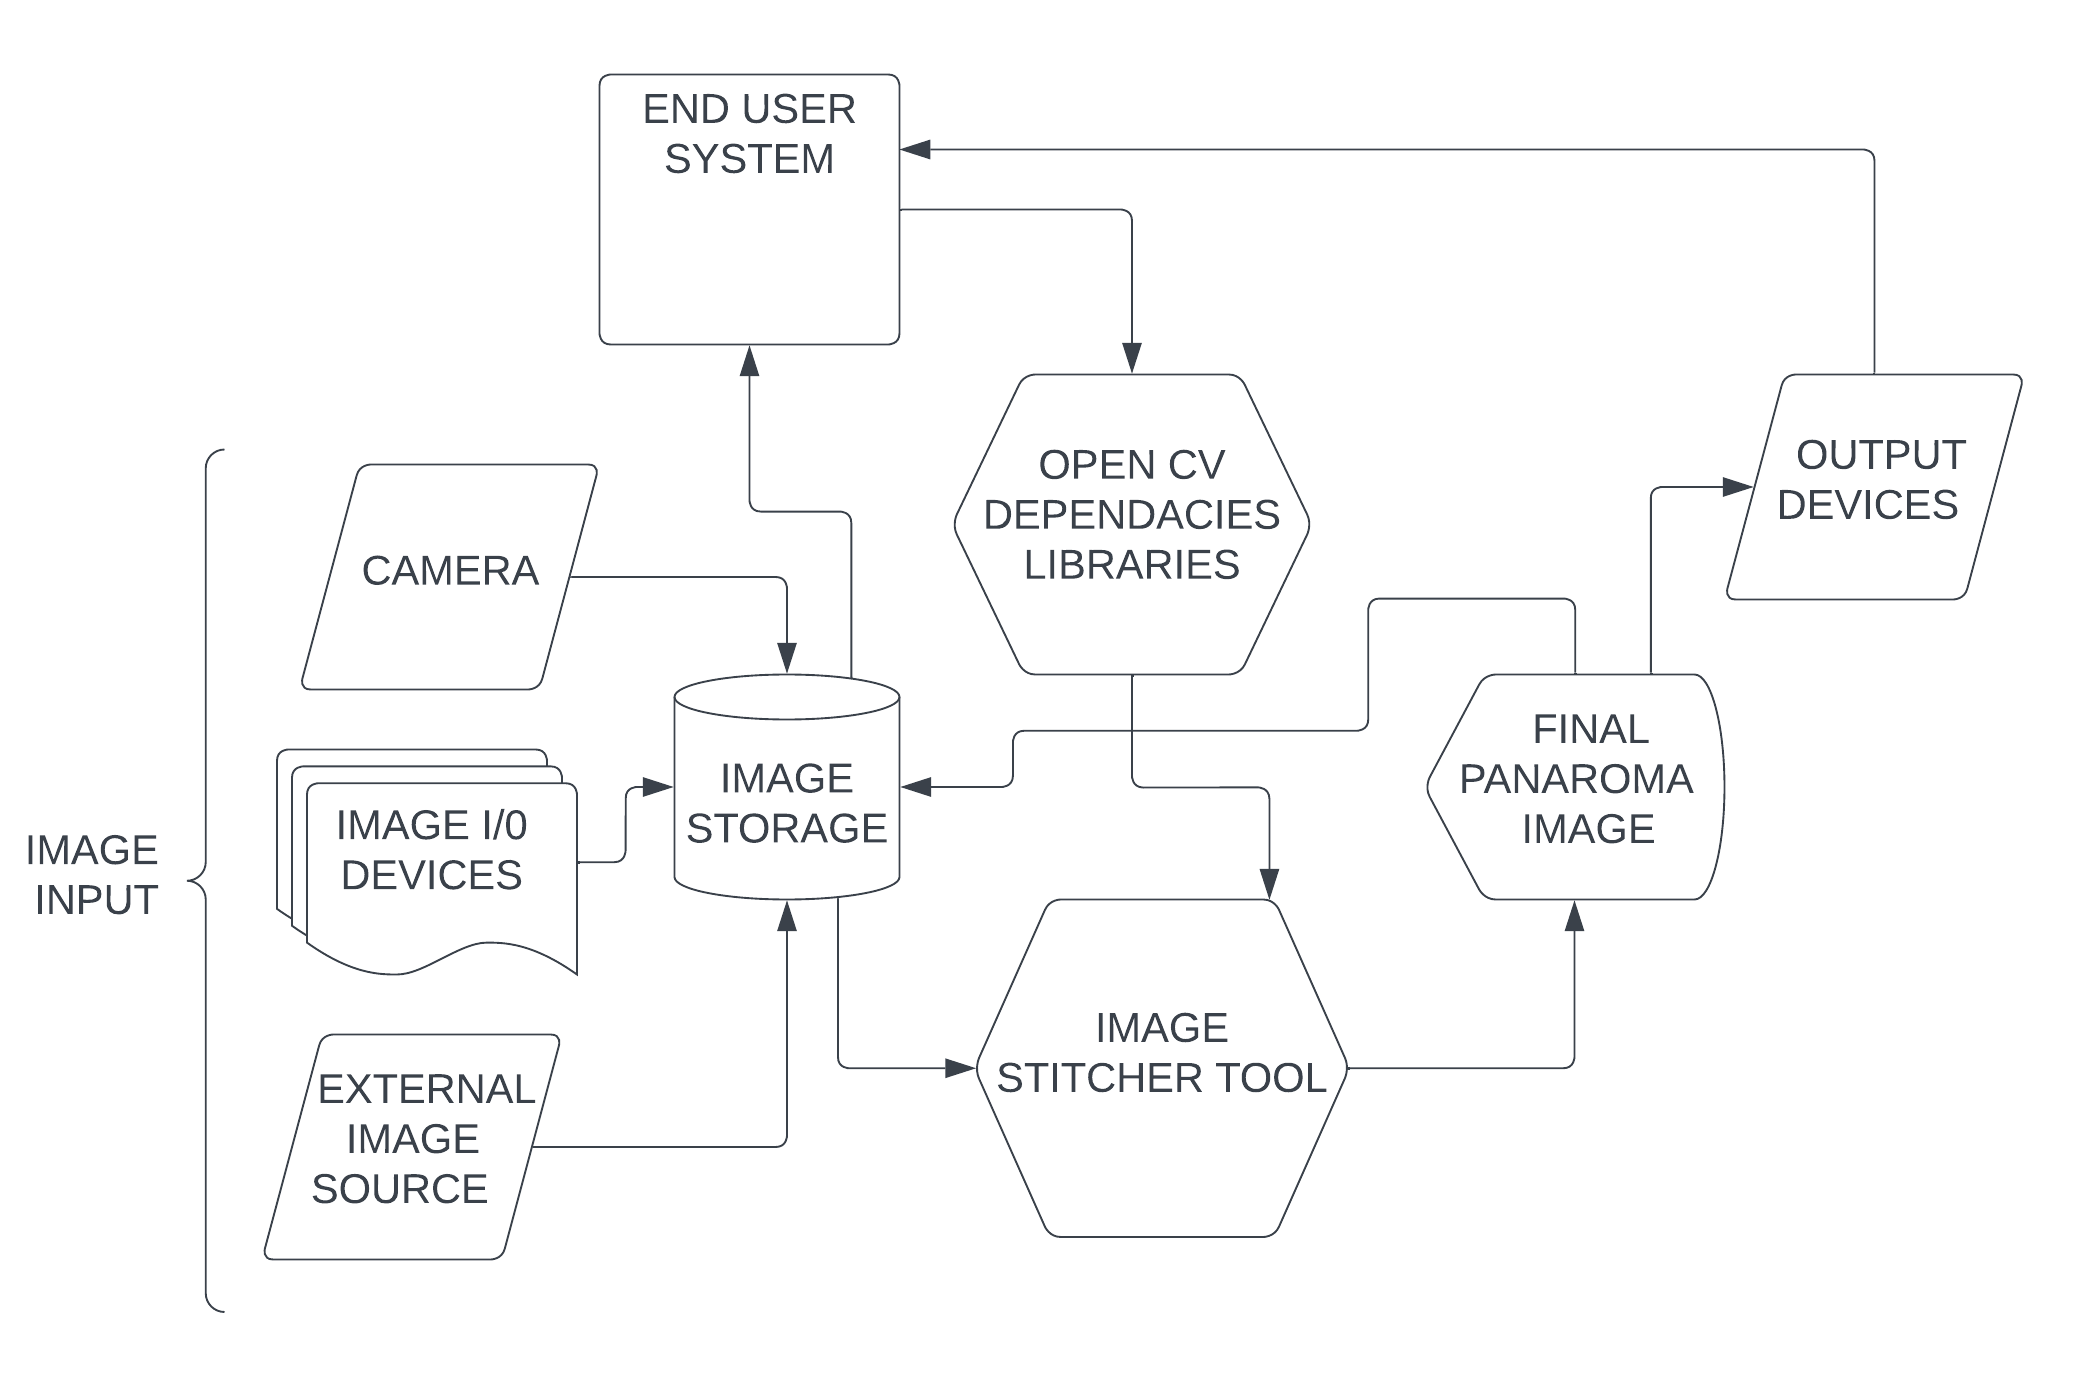
\includegraphics{Figures/DeploymentDiagram.png}}
     \caption{\label{Figure::DeploymentDiagram} Deployment Diagram of Image Stitching Module}
\end{figure}
The deployment view of OpenCV's image stitching module involves several components that work together to produce a final panorama output image: 
\begin{enumerate}
    \item Image input: The images that need to be stitched together.
    \begin{itemize}
        \item Camera: This is the device that captures the images that will be stitched together. 
        \item Image input/output devices: These are devices that can be used to input or output images, such as USB drives or SD cards. 
        \item External image source: This component refers to any external source of images that can be used as input for the stitching process.
    \end{itemize}
    \item Image storage database: This component is responsible for storing the images that will be used for stitching. It can be a local or remote database.

    \item OpenCV libraries / dependencies: This component includes all the necessary libraries and dependencies required for the image stitching module to function properly.

    \item Image Stitching module of OpenCV: This is the core component of the deployment view. It is responsible for stitching the input images together to produce a final panorama output image.

    \item Final panorama output image: This is the output of the image stitching module. It is the final image that is produced after the input images have been stitched together.

    \item Output devices: These are devices that can be used to output the final panorama image, such as a monitor or a printer.

    \item End-user system: This component refers to the system that the end-user will be using to access the image stitching module. It can be a desktop computer, a laptop, or a mobile device.
\end{enumerate}
Overall, the deployment view of OpenCV's image stitching module involves several components that work together to produce a final panorama output image. The input images can come from various sources, and the final output can be displayed on different output devices. The image stitching module is the core component that stitches the input images together, and the end-user system is the system that the end-user will be using to access the module.
\subsubsection{OpenCV Installation Dependencies\label{subsubSection::opencvInstallation}}
To install OpenCV on a system, there are several dependencies that need to be installed first. The specific dependencies required may vary depending on the operating system and the version of OpenCV being installed. Here is a general list of dependencies that are commonly required:
\begin{enumerate}
    \item CMake: This is a cross-platform build system that is used to build OpenCV from source.
    \item Git: This is a version control system that is used to download the OpenCV source code.
    \item GCC: This is a compiler that is used to compile the OpenCV source code.
    \item Python: OpenCV has a Python interface, so Python needs to be installed on the system.
    \item NumPy: This is a Python library that is used for numerical computing. It is required for the Python interface of OpenCV.
    \item libjpeg: This is a library for reading and writing JPEG files. It is required for the imgcodecs module of OpenCV.
    \item libpng: This is a library for reading and writing PNG files. It is required for the imgcodecs module of OpenCV.
    \item libtiff: This is a library for reading and writing TIFF files. It is required for the imgcodecs module of OpenCV.
    \item libjasper: This is a library for reading and writing JPEG-2000 files. It is required for the imgcodecs module of OpenCV.
    \item libwebp: This is a library for reading and writing WebP files. It is required for the imgcodecs module of OpenCV.
    \item OpenEXR: This is a library for reading and writing high dynamic range (HDR) images. It is required for the imgcodecs module of OpenCV.
    \item TBB: This is the Intel Threading Building Blocks library, which is used for parallel processing. It is required for the performance optimization of OpenCV.
    \item Eigen: This is a C++ template library for linear algebra. It is used for the computation of homography matrices in the image stitching process.
    \item CUDA: This is a parallel computing platform and programming model developed by NVIDIA. It is used for GPU acceleration in the image stitching process.
    \item OpenCL: This is an open standard for parallel programming of heterogeneous systems. It is used for GPU acceleration in the image stitching process.
\end{enumerate}
\pagebreak

\section{Summary of 4+1 View:\label{Section::Overview}}
Each view provides a distinct perspective on the OpenCV architecture, allowing stakeholders to understand and analyze the system from different angles. This 4+1 view model helps in capturing the functional, development, process, physical, and use case aspects of the OpenCV backend architecture.\\\\ \index{Backend}
Here is a diagram to showcase a brief overview of what we covered:

\begin{figure}[H]
     \centering
     \scalebox{0.23}{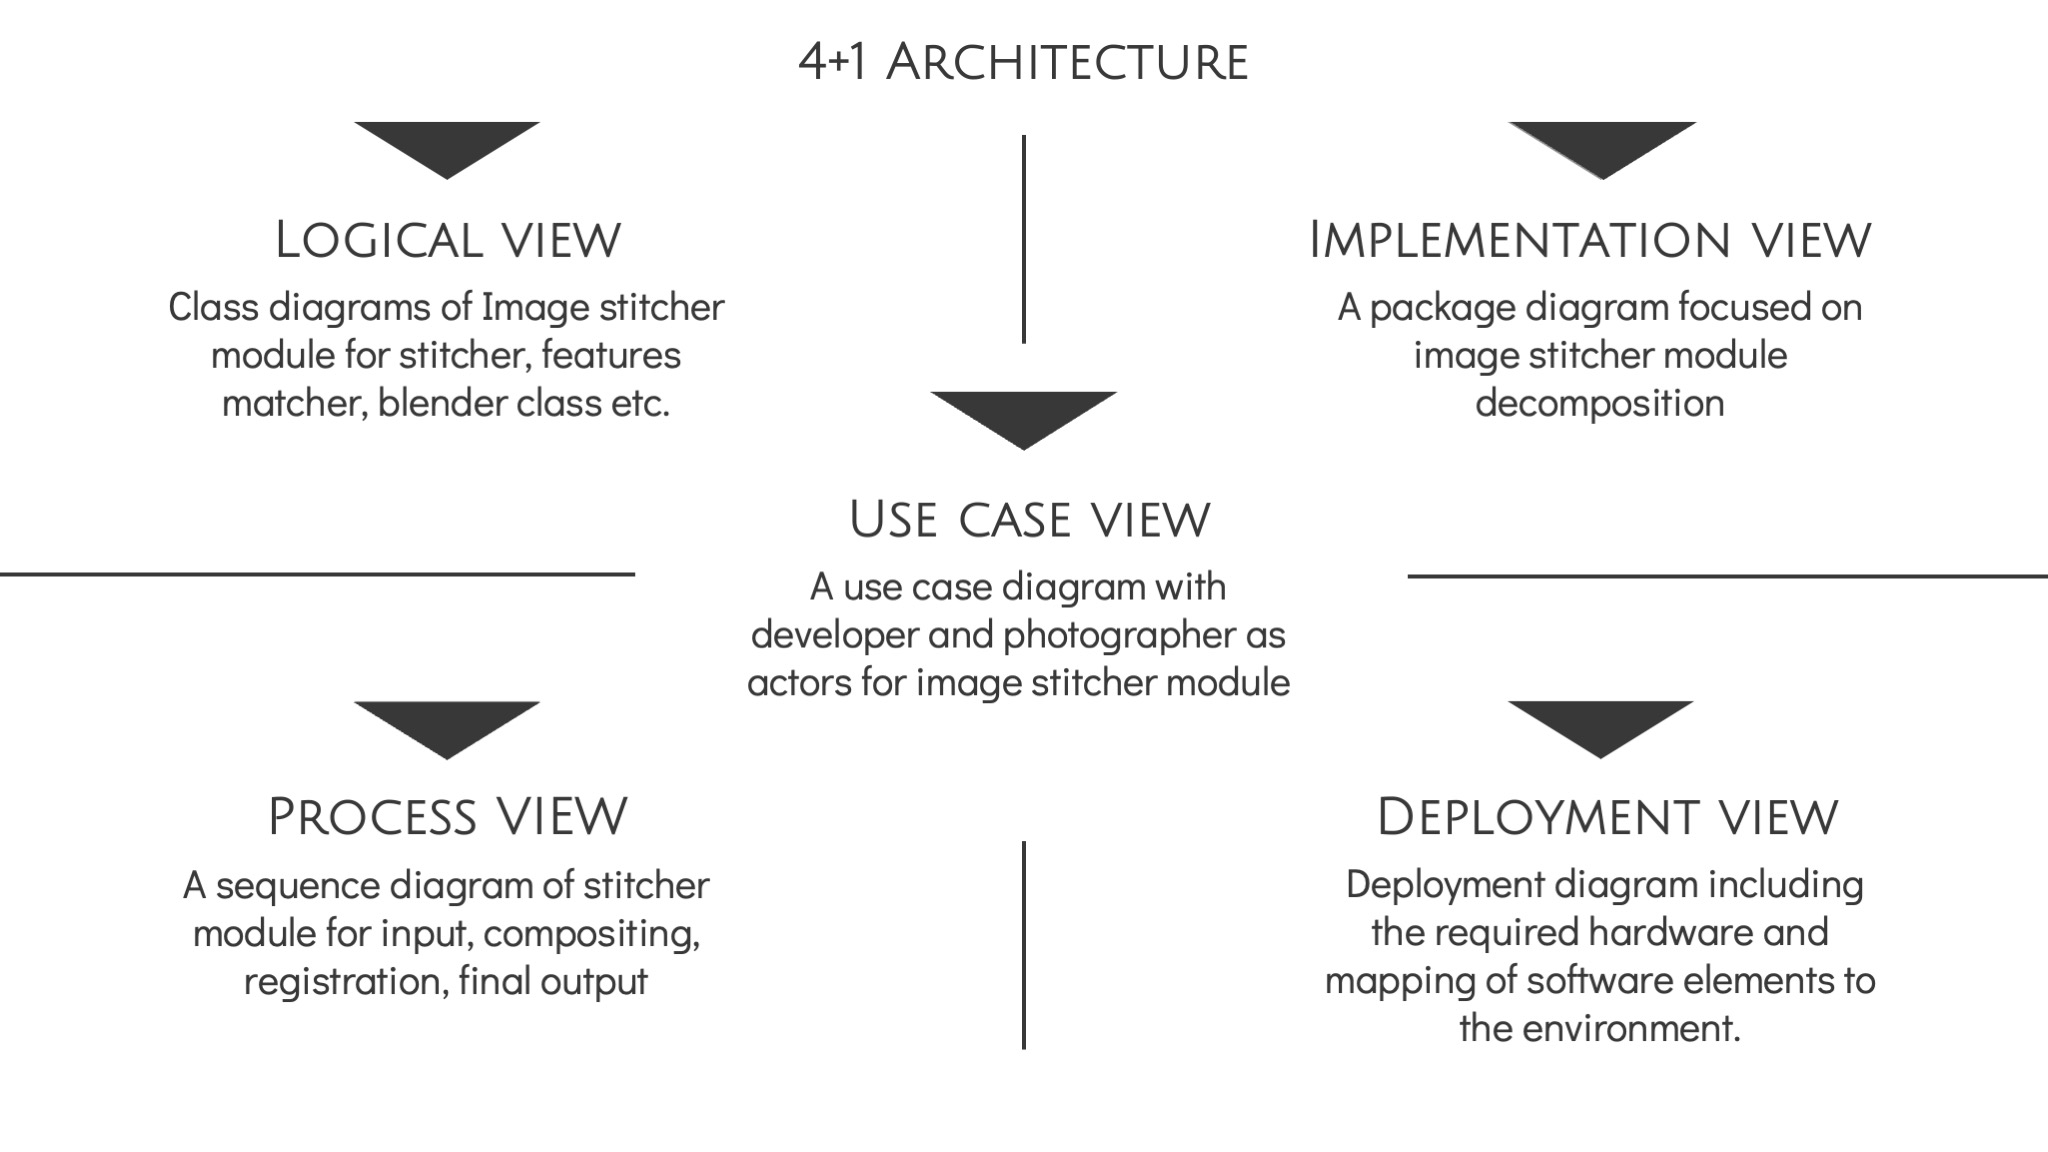
\includegraphics{Figures/BriefOverview.jpg}}
     \caption{\label{Figure::BriefOverview} 4+1 Overview}
\end{figure}
\par{The purpose of using the 4+1 view model for OpenCV's Image Stitching module is to provide a comprehensive understanding of the system's architecture from multiple perspectives. This approach helps to ensure that the system is designed and implemented in a way that meets the needs and requirements of its stakeholders, while also addressing potential risks and quality issues. \index{4+1 view}\\
\\
The Logical View provides a high-level overview of the system's functionality and the relationships between its components. This view focuses on the system's data and functionality, and how they are organized and structured. It helps stakeholders to understand the system's overall purpose and how it achieves its goals.\\
\\
The Process View describes the system's behavior and how it responds to external events. This view focuses on the system's processes and how they interact with each other and with external systems. It helps stakeholders to understand how the system works and how it responds to different inputs and events.\\
\\
The Implementation View describes the system's development environment and how it is organized. This view focuses on the system's development tools, processes, and methodologies. It helps stakeholders to understand how the system is developed and maintained, and how changes are made to the system over time.\\
\\
The Deployment View describes the system's physical architecture and how it is deployed. This view focuses on the system's hardware and software components, and how they are connected and configured. It helps stakeholders to understand how the system is deployed and how it interacts with other systems and devices.\\
\\
The Use Case View describes the system's functionality from the perspective of its users. This view focuses on the system's use cases and how they are implemented in the system. It helps stakeholders to understand how the system is used and how it meets the needs and requirements of its users.
\vspace{20pt}\\
Overall, the 4+1 view model provides a comprehensive understanding of the OpenCV Image Stitching module's architecture from multiple perspectives, helping stakeholders to understand the system's functionality, behavior, development environment, physical architecture, and user requirements. This understanding is essential for ensuring that the system is designed and implemented in a way that meets the needs and requirements of its stakeholders, while also addressing potential risks and quality issues.
}







\bibliography{bibfile}
%\bibliographystyle{unsrt}
\bibliographystyle{IEEEtran}

%% Initial version by Darian Muresan, Ph.D.
% Edit and adjust as needed.

\documentclass[12pt]{cornell}

% add index support
\makeindex

% graphing programs
\usepackage{color}
\usepackage{psfrag}
\usepackage{verbatim}
\usepackage{fancyhdr}
%\usepackage{titlesec}
\usepackage{fancyvrb} 
% hyperlink programs
\usepackage[pdfmark, 
breaklinks=true, 
colorlinks=true,
citecolor=blue,
linkcolor=blue,
menucolor=black,
pagecolor=black,
urlcolor=blue
]{hyperref} % links in pdf
%\usepackage[colorlinks]{hyperref} % links in dvi
\usepackage{listings}
\usepackage{amsfonts} 
\usepackage{amssymb} 
%\usepackage{tabto}

\usepackage{tabularx,colortbl}
\usepackage[chapter]{algorithm} 
\usepackage{algorithmic} 
\usepackage{blindtext}
\usepackage{imakeidx}


\definecolor{DarkGreen}{rgb}{0,0.6,0}
\definecolor{mygreen}{rgb}{0,0.6,0}
\definecolor{mygray}{rgb}{0.5,0.5,0.5}
\definecolor{mymauve}{rgb}{0.58,0,0.82}

\usepackage{tocloft}
\usepackage{amsmath}
\usepackage{tcolorbox}
\usepackage{enumitem}
\usepackage{longtable}
%\usepackage{textcomp}
\usepackage{txfonts}

%part for \part titles
%chap for \chapter titles
%sec for \section titles
%subsec for \subsection titles
%subsubsec for \subsubsection titles
%para for \paragraph titles
%subpara for \subparagraph titles
%fig for figure \caption titles
%subfig for subfigure \caption titles
%tab for table \caption titles
%subtab for subtable \caption titles

% update chapter number spacing
\setlength{\cftchapnumwidth}{2em}
\setlength{\cftsecnumwidth}{2.5em}
\setlength{\cftsubsecnumwidth}{3.5em}
\setlength{\cftsubsubsecnumwidth}{4.5em}

\addtolength{\cftsecindent}{0.5em}
\addtolength{\cftsubsecindent}{0.5em}
\addtolength{\cftsubsubsecindent}{0.5em}

%\titlespacing*{\chapter}{0pt}{-50pt}{20pt}
%\titleformat{\chapter}[display]{\normalfont\huge\bfseries}{\chaptertitlename\ 
%\thechapter}{20pt}{\Huge}
%\pagestyle{fancy}
%\pagestyle{cornell}
%
%\rhead{F054-021-0172}
%\chead{Nonlinear Enhancement of Visual Target Detection (AF05-T021)}
%\lhead{GSTI}
%\lfoot{\scriptsize Use or disclosure of data on this page is subject
%to the restriction on the title page of this proposal.}
%\cfoot{}
%\rfoot{\thepage}

\newfont{\Bp}{msbm10}
\newfont{\BpBig}{msbm10 scaled\magstep2}
\newfont{\Sc}{eusm10}
\newfont{\ScBig}{eusm10 scaled\magstep3}
\newfont{\Fr}{eufm10}
\newfont{\FrBig}{eufm10 scaled\magstep1}

% some commands:
\newcommand{\dxi}{{\tt m\_xDeltaInput}}
\newcommand{\dyi}{{\tt m\_yDeltaInput}}
\newcommand{\dci}{{\tt m\_cDeltaInput}}
\newcommand{\dxo}{{\tt m\_xDeltaOutput}}
\newcommand{\dyo}{{\tt m\_yDeltaOutput}}
\newcommand{\dco}{{\tt m\_cDeltaOutput}}
\newcommand{\ttf}[1]{{\tt #1}}
\newcommand{\tbl}[2]{{\begin{tabular}{c} #1 \\ #2 \end{tabular}}}

\newcommand{\urltwo}[2]{\mbox{\href{#1}{\tt #2}}}
\newcommand{\qnorm}[1]{\|#1\|_{\bQ}}
\newcommand{\qdot}[2]{\lrb #1, #2 \rrb_{\bQ}}
\newcommand{\kdot}[2]{\lrb #1, #2 \rrb_{\bf k}}
\newcommand{\tdot}[2]{\lrb #1, #2 \rrb}
\newcommand{\mydiff}[2]{\lrb #1 - #2 \rrb}
\newcommand{\lena}{\textit{lena}}
\newcommand{\barb}{\textit{barbara}}
\newcommand{\boat}{\textit{boat}}
\newcommand{\leaves}{\textit{leaves}}
\newcommand{\rings}{\textit{rings}}
\newcommand{\treg}{\textit{train region}}
\newcommand{\dreg}{\textit{denoise region}}
\newcommand{\oreg}{\textit{overlap region}}
\newcommand{\sil}{\sigma_l^2}
\newcommand{\sn}{\sigma^2}
\newcommand{\bn}{{\mbox{\bf \FrBig N}}}
\newcommand{\n}{\mbox{\Fr N}}
%\newcommand{\bn}{\bf N}
%\newcommand{\n}{N}
\newcommand{\bY}{\textbf{Y}}
\newcommand{\bX}{\textbf{X}}
\newcommand{\bb}{\textbf{b}}
\newcommand{\bu}{\textbf{u}}
\newcommand{\bv}{\textbf{v}}
\newcommand{\by}{\textbf{y}}
\newcommand{\bx}{\textbf{x}}
\newcommand{\be}{\textbf{e}}
\newcommand{\bz}{\textbf{z}}
\newcommand{\bs}{\textbf{s}}
\newcommand{\bw}{\textbf{w}}
\newcommand{\bQ}{\textbf{Q}}
\newcommand{\bphi}{\textbf{$\phi$}}
\newcommand{\lsb}{\left[}
\newcommand{\rsb}{\right]}
\newcommand{\lrb}{\left(}
\newcommand{\rrb}{\right)}
\newcommand{\lcb}{\left\{}
\newcommand{\rcb}{\right\}}
\newcommand{\R}{\mbox{\BpBig R}}
\newcommand{\F}{{\cal F}}
\newcommand{\Fk}{\mbox{\Sc F}}
\newcommand{\bQF}{\textbf{Q}_{\mbox{\Sc F}}}
\newcommand{\N}{{\cal N}}
\newcommand{\xlz}{X_l(z)}
\newcommand{\xhz}{X_h(z)}
\newcommand{\xz}{X(z)}
\newcommand{\pr}{ perfect reconstruction }
\newcommand{\smb}{Smith-Barnwell }
\newcommand{\xw}{X(e^{j\omega})}
\newcommand{\xmw}{X(-e^{j\omega})}
\newcommand{\dw}{D(e^{j\omega})}
\newcommand{\dmw}{D(-e^{j\omega})}
\newcommand{\ew}{E(e^{j\omega})}
\newcommand{\emw}{E(-e^{j\omega})}
\newcommand{\fw}{F_0(e^{j\omega})}
\newcommand{\fmw}{F_0(-e^{j\omega})}
\newcommand{\hoz}{H_1(z)}
\newcommand{\hzz}{H_0(z)}
\newcommand{\goz}{G_1(z)}
\newcommand{\gzz}{G_0(z)}
\newcommand{\hzw}{H_{0}(e^{j\omega})}
\newcommand{\hzmw}{H_{0}(-e^{j\omega})}
\newcommand{\hzcw}{H_{0}(e^{-j\omega})}
\newcommand{\how}{H_1(e^{j\omega})}
\newcommand{\homw}{H_1(-e^{j\omega})}
\newcommand{\gzw}{G_0(e^{j\omega})}
\newcommand{\gzmw}{G_0(-e^{j\omega})}
\newcommand{\gow}{G_1(e^{j\omega})}
\newcommand{\gomw}{G_1(-e^{j\omega})}
\newcommand{\wl}{e^{-jwL}}
\newcommand{\aqua}{\textit{AQua with OR }}
\newtheorem{theorem}{Theorem}
\newtheorem{lemma}{Lemma}
\newtheorem{corollary}{Corollary}
\newtheorem{claim}{Claim}
\newtheorem{definition}{Definition}
\newenvironment{proof}{\noindent{\em Proof.}}{\ \hfill Q.E.D.}
%\newtheorem{moduleCount}{L}
\newcommand*{\labelfile}[1]{%
  \label{file:#1}%
}

\lstset{ %
  backgroundcolor=\color{white},   % choose the background color; you must add \usepackage{color} or \usepackage{xcolor}
  basicstyle=\footnotesize,        % the size of the fonts that are used for the code
  breakatwhitespace=false,         % sets if automatic breaks should only happen at whitespace
  breaklines=true,                 % sets automatic line breaking
  captionpos=b,                    % sets the caption-position to bottom
  commentstyle=\color{DarkGreen},    % comment style
  deletekeywords={...},            % if you want to delete keywords from the given language
  escapeinside={\%*}{*)},          % if you want to add LaTeX within your code
  extendedchars=true,              % lets you use non-ASCII characters; for 8-bits encodings only, does not work with UTF-8
  %frame=single,                   % adds a frame around the code
  keepspaces=true,                 % keeps spaces in text, useful for keeping indentation of code (possibly needs columns=flexible)
  keywordstyle=\color{blue},       % keyword style
  language=C++,                    % the language of the code
  morekeywords={*,...},            % if you want to add more keywords to the set
  numbers=left,                    % where to put the line-numbers; possible values are (none, left, right)
  numbersep=5pt,                   % how far the line-numbers are from the code
  numberstyle=\tiny\color{mygray}, % the style that is used for the line-numbers
  rulecolor=\color{black},         % if not set, the frame-color may be changed on line-breaks within not-black text (e.g. comments (green here))
  showspaces=false,                % show spaces everywhere adding particular underscores; it overrides 'showstringspaces'
  showstringspaces=false,          % underline spaces within strings only
  showtabs=false,                  % show tabs within strings adding particular underscores
  stepnumber=1,                    % the step between two line-numbers. If it's 1, each line will be numbered
  stringstyle=\color{mymauve}     % string literal style
  %tabsize=2,                      % sets default tabsize to 2 spaces
  %caption=\lstname                % show the filename of files included with \lstinputlisting; also try caption instead of title
}

% Uncomment draftcopy to get the word DRAFT boldly across the first page
%   By the way, xdvi won't show it but it will come out when you print
%\usepackage[light,all]{draftcopy}		% DRAFT on first page
%\draftcopySetGrey{.97}
%\draftcopyName{Confidential}{150}
%\draftcopFirstPage{1}

% Uncomment drafthead to get the date and DRAFT in the header of pages
% that are normallly numbered on the top, pages 2-n of each chapter for example
% This doesn't work with centered page numbers: \pagestyle{cornellc}
%\usepackage{drafthead}

% Including selective chapters:
% use this to selectively process chapters, etc.  Put a % in front of
% the sections that you don't want done this time.  Includes are
% used instead of \input so that LaTeX will keep track of chapters and
% pages without processing everything.  Don't let any spaces creep in
% around the words or it will not work!


\includeonly{
prologue,
manIntroduction,
ProjectProposalWeek5,
ProjectSummary,
Objective,
Stakeholders,
UserStories,
BusinessRequirements,
UserRequirements,
Quality Attributes,
Risks,
Architecture
}

\makeindex[program=makeindex,options=-s pyro,columns=2,intoc=true]

\begin{document}

\pagenumbering{roman}
\singlespacing
% File: prologue.tex
% Thesis prologue:  Title page, acknowledgements, table of contents,
% list of figures, and list of tables.
%
% this file is to be \include'd after the \begin{document}

% Cornell-style title page
\begin{figure}[H]
            \centering
            \scalebox{0.2}{
\includegraphics{Figures/Stevens.png}}
\end{figure}
\begin{titlepage}
        \title{ Final Project Report: OpenCV }
        
        \author{Nikhil Kumar G and Raj Palival \\ Course Instructor: David Darian Muresan \\ Course Name: Software Architecture SSW565  \\
        \MakeUppercase {Stevens Institute of Technology}\\
        Castle Point on Hudson \\
        Hoboken, NJ 07030 }
        \conferraldate{}{May 15, 2023} \maketitle
\end{titlepage}

% Copyright page
%\begin{copyrightpage}
\makecopyright
%\end{copyrightpage}

% Abstract: the abstract body is pulled from the file abstract.tex;
%  the title is pulled from the \title command in the titlepage section
\begin{abstract}
        %\makeabstitle
        \input abstract      % puts the abstract file here
\end{abstract}

% Biographical information pulled from file bio.tex
%\begin{biosketch} \input bio \end{biosketch}

% Dedication (optional):  pulls information from file dedication.tex
%\begin{dedication} 
%\input dedicate 
%\end{dedication}

% Acknowledgements:  pulls information from file acknow
%\begin{acknowledgements} \input acknow \end{acknowledgements}

% Table of contents
\contentspage

% If you have no tables or figures put a % in front of the list page line
% List of tables
\tablelistpage

% List of figures
\figurelistpage



\setcounter{page}{1}        % set page counter
\pagenumbering{arabic}      % set page number style
\pagestyle{fancy}         % top right page numbers
%\pagestyle{cornell}
%\pagestyle{cornellc}       % centered page numbers, disables drafthead

\renewcommand{\chaptermark}[1]{\markboth{#1}{}}
\renewcommand{\sectionmark}[1]{\markright{#1}{}}

\fancyhead{} % clear all fields

\lhead{Chapter \thechapter}
%\lhead{\thechapter}
\chead{\leftmark}
\rhead{\thepage}


\lfoot{Chapter \thechapter}
\cfoot{\copyright Stevens -- \today \mbox{} -- OpenCV}
\rfoot{\thepage}

\renewcommand{\headrulewidth}{0.4pt}
\renewcommand{\footrulewidth}{0.4pt}

%\rhead{F054-021-0172}
%\chead{Nonlinear Enhancement of Visual Target Detection (AF05-T021)}
%\lhead{GSTI}
%\lfoot{\scriptsize Use or disclosure of data on this page is subject
%to the restriction on the title page of this proposal.}
%\cfoot{}
%\rfoot{\thepage}


\singlespacing
\chapter{Team Members Introduction \\
\small{\textit{-- Nikhil Kumar G, Raj Palival}} 
\index{Chapter!Introduction}
\index{Introduction}
\label{Chapter::Introduction}}

% Add a section and label it so that we can reference it later
\section{Nikhil Kumar G \label{Section::chp1NikhilIntro}}
I'm pursuing my masters in Software Engineering\index{Software Engineering} at SSE\index{SSE}. I've always had a natural tendency to think very logically which has driven me to pursue this degree. Considering all the major ongoing technological advancements, I believe we can offer the future a lot more than we can imagine.\\
I have worked as an intern on "Home automation and Security Systems"\index{Home automation} \index{Security Systems} at a startup business "Li2 Technologies". \index{Li2 Technologies} After finishing my undergrad studies, I started working at "Accenture", \index{Accenture} where I spent more than a year creating Java, OIC, and SOA services. \index{Java} \index{OIC} \index{SOA}

\section{Raj Palival \label{Section::chp1RajIntro}}
I am currently pursuing my masters in Software Engineering from Stevens Institute of Technology. My background work experience was working as a software devloper in Health sector domain, During my time here I have helped automate the front-end queries \index{Front-End Queries} of our web application called 'GuidingCare' using Structured Rule Language in FICO Blaze system \index{FICO Blaze System}. I am looking forward to finish this degree with high honors and continue to work in computer science division as a software devloper and create meaningful applications.

\chapter{Project Proposal\\
\small{\textit{-- Nikhil Kumar G, Raj Palival}}
\index{Chapter!Project Proposal}
\index{Project Proposal}
\label{Chapter::Project Proposal}}

\section{Open Source Project: Open CV \label{Section::chp2OpenCV}}
\subsection{Description}
The open source project that we have chosen for the project evaluation\index{Evaluation} is "OpenCV.org" \cite{OCV}.
As we have personally used Open CV for projects before, we recognize its importance and we are familiar with its functionality\index{Functionality} to go ahead with it.\\ 
\\
\begin{figure}[ht]
\centering
\scalebox{0.4}{
\includegraphics{Figures/Logo.png}}
\caption{\label{Figure::OpenCVlogo} Open CV Logo}
\end{figure}
\\
OpenCV (Open Source Computer Vision Library) is an open source computer vision\index{Computer Vision} and machine learning\index{Machine Learning} software library. OpenCV was built to provide a common infrastructure\index{Infrastructure} for computer vision applications and to accelerate the use of machine perception\index{Machine Perception} in the commercial products. Being an Apache 2\index{Apache 2} licensed product, OpenCV makes it easy for businesses to utilize and modify the code \cite{6240859}. 
\chapter{Summary\\
\small{\textit{-- Nikhil Kumar G, Raj Palival}}
\index{Chapter!Summary}
\index{Summary}
\label{Chapter::Summary}}

\par{The purpose of this document is to provide a overview of openCV's architecture and a comprehensive overview of the software architecture for OpenCV's Image Stitching module \cite{openCVReport}. The document outlines the key stakeholders, user requirements, business requirements, quality attributes \cite{qualityattributes}, and risks involved in the system, and provides a detailed description of the architecture from multiple perspectives. The document is intended to serve as a reference for developers, project managers, and other stakeholders who need to understand the system and its architecture. By providing a clear and detailed description of the system's architecture, the document helps ensure that the system is designed and implemented in a way that meets the needs and requirements of its stakeholders, while also addressing potential risks and quality issues. Overall, the purpose of this document is to facilitate effective communication and collaboration among stakeholders, and to ensure the successful development and deployment of the OpenCV Image Stitching module.}\\

\par{Overall, the 4+1 view model provides a comprehensive understanding of the OpenCV Image Stitching module's architecture from multiple perspectives, helping stakeholders to understand the system's functionality, behavior, development environment, physical architecture, and user requirements. This understanding is essential for ensuring that the system is designed and implemented in a way that meets the needs and requirements of its stakeholders, while also addressing potential risks and quality issues.
}
\chapter{Objective\\
\small{\textit{-- Nikhil Kumar G, Raj Palival}}
\index{Chapter!Objective}
\index{Objective}
\label{Chapter::Objective}}

\section{OpenCV\label{openCVObjective}}
The objective of OpenCV architecture is to provide a flexible and modular framework for computer vision applications \cite{sampleArch}. The architecture is designed to be highly customizable and extensible, allowing developers to easily integrate new functionalities and algorithms into their applications. The architecture also provides a set of core modules that cover a wide range of computer vision tasks, such as image processing, feature detection, object recognition, and machine learning.\\These modules are designed to be efficient and optimized for performance, making them suitable for real-time applications. Additionally, the architecture provides a user-friendly interface and intuitive APIs that make it easy for developers to interact with the library and implement their computer vision projects. Overall, the objective of OpenCV architecture is to provide a powerful and flexible tool for computer vision applications that can be tailored to meet the specific needs and requirements of each project. 
\index{modular framework} \index{APIs}\index{pairwise stitching}\index{multi-band blending}\index{multi-row stitching}\index{user-friendly interface}
\section{OpenCV Image-Stitching Module\label{imageStitchObjective}}
The objective of the OpenCV image stitching module is to provide a set of tools and algorithms for stitching multiple images together to create a panoramic image. The module is designed to be efficient and optimized for performance, making it suitable for real-time applications. The module provides a set of core functionalities, such as feature detection, feature matching, and image blending, that are used to align and blend the input images into a seamless panoramic image.\\
\\The module also provides various stitching methods, such as pairwise stitching, multi-row stitching, and multi-band blending, that can be used to achieve different levels of quality and performance. Additionally, the module provides a user-friendly interface and intuitive APIs that make it easy for developers to interact with the library and implement their image stitching projects. Overall, the objective of the OpenCV image stitching module is to provide a powerful and flexible tool for creating panoramic images that can be tailored to meet the specific needs and requirements of each project.
\chapter{Stakeholders\\
\small{\textit{-- Nikhil Kumar G, Raj Palival}}
\index{Chapter!Stakeholders}
\index{Stakeholders}
\label{Chapter::Stakeholders}}

\section{Introduction \label{Section::StakeholdersIntroduction}}
In this chapter, we are going to learn about the stakeholders of Open CV. Stakeholders in general for OpenCV can be classified as people or roles who are affected, in some way, by OpenCV. Also, it's worth noting that stakeholders may vary over time as the OpenCV community and ecosystem evolve.

\section{Types of Stakeholders \label{Section::StakeholdersType}}
We will try to group the stakeholders of OpenCV into two broad categories:
\begin{enumerate}
     \item OpenCV Builders
     \item OpenCV Users
 \end{enumerate}
 
\subsection{OpenCV Builders \label{subSection::OpenCVBuilders}}
These stakeholders are involved in developing, maintaining, and enhancing the OpenCV library. They contribute to its code-base, research and implement new algorithms, and ensure its continuous development. The potential stakeholders involved in building OpenCV are:
\begin{enumerate}
     \item Developers
     \item Contributors
     \item OpenCV Foundation
     \item Open-Source community
 \end{enumerate}

 \subsection{OpenCV Users \label{subSection::OpenCVUsers}}
These stakeholders utilize the OpenCV library for various computer vision tasks and applications. They leverage the functionality provided by OpenCV in their projects, products, or services. They can be sub-divided into an exhaustive list. Hence, the potential stakeholders involved in using OpenCV are:
\begin{enumerate}
     \item End-Users
     \item Researchers
     \item Academic institutions
     \item Industry partners
     \item Government agencies
 \end{enumerate}
\index{OpenCV Foundation}\index{Open-Source community}\index{End-Users}\index{Researchers}\index{Academic institutions} \index{Industry partners}\index{Government agencies}\index{bug reports}
\begin{table} [H]
\begin{tabular}{|c|m{11.4cm}|} 
\hline
\textbf{STAKEHOLDERS} & \textbf{DESCRIPTION} \\ \hline
Developers & Developers are the core team responsible for actively developing, maintaining, and enhancing the OpenCV library's source code and features. \\ \hline 

Contributors & They are individuals or organizations who support the project by providing bug reports, feedback, documentation, tutorials, and code changes, helping to improve and expand its functionality. \\ \hline 

OpenCV Foundation & The organization responsible for managing and overseeing the development and maintenance of the OpenCV library, ensuring its long-term sustainability and growth. \\ \hline 

Open-Source Community & The broader community of developers, enthusiasts, and users who provide feedback, support, and contribute to the improvement and expansion of OpenCV. \\ \hline 

End-Users & The ultimate beneficiaries or users of the project's outcome, who will interact with the OpenCV-based functionalities directly or indirectly. \\ \hline 

Researchers & Professionals and academics who employ OpenCV in their research work, leveraging its computer vision algorithms and functionalities. \\ \hline 

Academic Institutions & Universities and research institutes that incorporate OpenCV into their computer vision courses and projects, helping educate future computer vision professionals. \\ \hline 

Industry Partners & Companies and organizations that integrate OpenCV into their products, services, or platforms, enabling computer vision capabilities. \\ \hline 

Government Agencies & Public sector organizations that may utilize OpenCV for various purposes, such as surveillance, image analysis, or research initiatives. \\ \hline 
\end{tabular}
\caption{Stakeholders' description \label{Table::StakeholdersDescription}}
\end{table}

\chapter{User Stories\\
\small{\textit{-- Nikhil Kumar G, Raj Palival}}
\index{Chapter!User Stories}
\index{User Stories}
\label{Chapter::User Stories}}

\section{What is a User Story ? \label{Section::UserStoriesIntroduction}}
A user story is a small, self-contained unit of development work designed to accomplish a specific goal within a product. A user story is usually written from the user’s perspective and follows the format: “As [a user persona], I want [to perform this action] so that [I can accomplish this goal].”\newline
\newline
User stories:
\begin{itemize}
\item Are easy for anyone to understand
\item Represent bite-sized deliverables that can fit in sprints, whereas not all full features can. \index{bite-sized deliverables}
\item Help the team focus on real people, rather than abstract features
\item Build momentum by giving development teams a feeling of progress
\end{itemize}
\section{User Stories\label{Section::UserStories}}
\begin{enumerate}
    \item As a developer, I want to use OpenCV to easily integrate computer vision capabilities into my software applications, so that I can create more advanced and intelligent applications that can analyze and interpret visual data.
    \item As a contributor, I want to contribute to the development of OpenCV by submitting bug reports, fixing issues, and adding new features, so that I can help improve the quality and functionality of the software for the benefit of the community.
    \item As the OpenCV foundation, we want to promote the use and development of OpenCV by providing resources, support, and guidance to developers, researchers, and industry partners, so that we can advance the field of computer vision and make it more accessible to everyone.
    \item As a member of the open source community, I want to collaborate with other developers and contributors to improve OpenCV, share my knowledge and expertise, and help make computer vision more accessible and useful to everyone.
    \item As an end-user, I want to use OpenCV to solve real-world problems, such as object recognition, face detection, and image processing, so that I can improve my productivity, efficiency, and quality of life.
    \item As a researcher, I want to use OpenCV to conduct experiments, analyze data, and develop new algorithms and techniques in the field of computer vision, so that I can advance the state of the art and contribute to the scientific community \cite{888718}.
    \item As an academic institution, we want to use OpenCV to teach computer vision concepts and techniques to our students, conduct research, and collaborate with other institutions and industry partners, so that we can prepare our students for careers in this rapidly growing field \cite{9103956}.
    \item As an industry partner, we want to use OpenCV to develop innovative products and services that leverage computer vision technology, so that we can improve our competitiveness, create new business opportunities, and provide value to our customers \cite{8097324}.
    \item As a government agency, we want to use OpenCV to develop solutions that can help us address various challenges, such as public safety, transportation, and environmental monitoring, so that we can improve the quality of life for our citizens and promote economic growth.
\end{enumerate}
\chapter{Business Requirements\\
\small{\textit{-- Nikhil Kumar G, Raj Palival}}
\index{Chapter!Business Requirements}
\index{Business Requirements}
\label{Chapter::Business Requirements}}

\section{Introduction \label{Section::BusinessRequirementIntro}} \index{Business Requirements}
Business requirements outline a project's needs and prerequisites for success while taking the target audience into account. It explains the rationale behind developing a certain project, who will use it, what advantages users will experience, and how the project's success will be measured. Business requirements do not specify how the project is to be developed \cite{businessRequirement}.
\subsection{What does a business requirement include ?\label{SubSection::BRInclusions}}
\begin{itemize}
    \item Key objectives and identification of a problem.
    \item Benefits of the proposed solution.
    \item Project scope.
    \item Rules, regulations, and policies.
    \item Key features of the project.
    \item Performance and security features.
    \item Metrics to measure the success of the project.
\end{itemize}
\subsection{What does a business requirement not include ?\label{SubSection::BRExclusions}}
\begin{itemize}
    \item Details of the functional requirements of the system.
    \item Details of the implementation of functional or performance requirements.
    \item Details of how to implement policies and regulations.
\end{itemize}
\newpage
\section{Business Requirements\label{Section::BusinessRequirements}}
\begin{enumerate}
    \item Open source: Develop and maintain an open source computer vision and machine learning software library that provides a common infrastructure for computer vision applications, which will allow developers to contribute to the project and make it better. This will also make OpenCV more accessible to a wider range of developers.
    \item Real-time performance: OpenCV must be able to process images and videos in real time, which is essential for many applications such as facial recognition, object detection, and video surveillance.
    \item Documentation: OpenCV must have comprehensive documentation, which will help developers learn how to use the library. This will make it easier for developers to get started with OpenCV and build their applications.
    \item Image Processing: OpenCV should be able to process images of various formats, including JPEG, PNG, and BMP. It should be able to perform basic image processing operations such as resizing, cropping, and rotating images. Additionally, it should be able to apply filters such as blur, sharpen, and edge detection to images.
    \item Hardware acceleration: OpenCV must support hardware acceleration, such as CUDA and OpenCL, to improve performance. This will allow developers to take advantage of the latest hardware to speed up their applications. \index{Hardware acceleration} \index{CUDA} \index{OpenCL} \index{video surveillance}
    \item Support: OpenCV should have a strong support system that provides timely and effective assistance to users. It should have a large and active community forum where users can ask questions and share their experiences. It should also have a dedicated support team that can help users troubleshoot issues and provide solutions to problems.
    \item Cross-platform compatibility: Develop and maintain a computer vision and machine learning software library that can be used on various platforms, including Windows, Linux, Android, and Mac OS. This will allow developers to use OpenCV on a variety of devices and systems. \index{Cross-platform} \index{Windows} \index{Linux} \index{Android} \index{Mac OS}
    \item Lowering costs: Enable businesses to utilize and modify the code for their specific needs, without incurring high licensing costs.
    \item Multi-Language Support: Ensure compatibility with popular programming languages, including C++, Python, Java, and MATLAB. \index{C++} \index{Python} \index{Java} \index{MATLAB} \index{Customization} \index{filters}
    \item Customization: OpenCV should be customizable to meet the specific needs of the business. It should allow users to create custom filters, algorithms, and models. It should also allow users to modify the user interface to suit their preferences and workflows.
\end{enumerate}
\chapter{User Requirements\\
\small{\textit{-- Nikhil Kumar G, Raj Palival}}
\index{Chapter!User Requirements}
\index{User Requirements}
\label{Chapter::User Requirements}}

\section{What is a User Requirement? \label{Section::UserRequirementsIntroduction}}
In this chapter, we are going to learn about the 'User Requirements' of OpenCV. User requirements are detailed and specific statements that outline the functionality, constraints, and qualities expected from a system or product. 

\section{User Requirements of OpenCV \label{Section::UserRequirements}}
Users often have certain expectations and needs when utilizing OpenCV in their projects. Some common user requirements of OpenCV can include:
\begin{longtable}{| p{.21\textwidth} | p{.79\textwidth} |} 
\hline
\textbf{User requirements} & \textbf{Description}  \\ \hline
Versatile Image and Video Processing & Users expect OpenCV to provide a wide range of image and video processing capabilities, such as image filtering, resizing, color space conversions, object detection, and tracking. \\ \hline 
Efficient and Optimized Algorithms & Users require efficient and optimized algorithms implemented in OpenCV, enabling fast and accurate computer vision operations even on resource-constrained devices. \\ \hline
Robust and Accurate Functions & Users depend on OpenCV to deliver reliable and accurate computer vision functions, such as feature extraction, pattern recognition, image segmentation, and optical flow analysis. \\ \hline
Documentation and Support & Users look for comprehensive documentation, tutorials, and examples that help them understand and effectively use the OpenCV library. They also appreciate active community support, forums, and resources that assist in troubleshooting and problem-solving. \\ \hline
Cross-Platform Compatibility & Users expect OpenCV to work seamlessly across different platforms and operating systems, including Windows, macOS, Linux, Android, and iOS. \\ \hline
Integration with Libraries and Frameworks & Users often require OpenCV to integrate smoothly with other libraries and frameworks commonly used in computer vision and machine learning, such as NumPy, TensorFlow, and PyTorch. \\ \hline
Flexibility and Customization & Users appreciate the ability to customize and extend OpenCV to suit their specific project requirements, including the option to add new algorithms, modify existing functions, or interface with specialized hardware. \\ \hline
Performance Optimization Tools & Users often require tools and techniques to optimize the performance of OpenCV-based applications, including multi-threading, GPU acceleration, and code profiling. \\ \hline
License Compatibility & Users may have specific requirements regarding the licensing of OpenCV to ensure compliance with their project's open-source or commercial license obligations. \\ \hline
Real-Time Camera & Users require OpenCV to provide seamless integration with cameras and enable real-time capture and processing of camera input. \\ \hline 
\caption{User Requirements \label{Table::UserRequirements}}
\end{longtable}

These user stories demonstrate the diverse range of users and their specific needs when utilizing OpenCV for various applications, spanning from research and development to commercial projects and personal interests.
\chapter{Quality Attributes\\
\small{\textit{-- Nikhil Kumar G, Raj Palival}}
\index{Chapter!Quality Attributes}
\index{Quality Attributes}
\label{Chapter::Quality Attributes}}

\section{Introduction\label{Section::QAIntro}}
\begin{quote}
Quality is never an accident; it is always the result of high intention, sincere effort, intelligent direction and skillful execution. 
\end{quote}
\begin{flushright}
- William A. Foster
\end{flushright}
Non-functional requirements (NFRs) define the criteria that are used to evaluate the whole system, but not for a specific behavior, and are also called quality attributes and described in detail in architectural specifications.
\\
All NFRs can be divided into two main categories:
\begin{enumerate}
\item NFRs that affect system behavior, design, and user interface during work.
\item NFRs that affect the development and support of the system.
\end{enumerate}
\section{Quality Attribute Scenario\label{Section::QAScenarios}}
A common form to specify all QA requirements as scenarios. The common form is testable and unambiguous; Thus it provides regularity in how we treat all quality attributes.
\\
Quality attribute scenarios have six parts:
\begin{enumerate}
    \item Source of stimulus: This is some entity (a human, a computer system, or any other actuator) that generated the stimulus.
    \item Stimulus: The stimulus is a condition that needs to be considered when it arrives at a system.
    \item Artifact: Some artifact is stimulated. This may be the whole system or some pieces of it.
    \item Environment: The stimulus occurs within certain conditions. The system may be in an overload condition or may be running when the stimulus occurs, or some other condition may be true.
    \item Response: The response is the activity undertaken after the arrival of the stimulus.
    \item Response measure: When the response occurs, it should be measurable in some fashion so that the requirement can be tested.
\end{enumerate}
\begin{figure}
\centering
\scalebox{1.0}{\includegraphics{Figures/qualityattributescenario.jpg}}
\caption{\label{Figure::The parts of a quality attribute scenario} The parts of a quality attribute scenario.}
\end{figure}
\index{Non-functional requirements}\index{testable}\index{unambiguous}\index{Source of stimulus}\index{Stimulus}\index{Environment}\index{Response}\index{Response measure}\index{uptime}\index{error rate}\index{Scenario}
\section{List of Significant Quality Attribute Scenarios\label{Section::SignificantQAS}}
\subsection{Availability\label{subSection::AvailabilityQA}}
\begin{enumerate}
    \item Source of stimulus: A user requests to stitch two images together.
    \item Stimulus: The user clicks on a button to start the stitching process.
    \item Artifact: The two images that the user wants to stitch together.
    \item Environment: The OpenCV Image Stitcher module is running on a computer.
    \item Response: The Image Stitcher module stitches the two images together and displays the result.
    \item Response measure:
    \begin{itemize}
        \item The response measure is the time it takes to stitch the two images together.
        \item The percentage of time that the library is able to process requests and return results without any errors or downtime.
        \item This can be measured using metrics such as uptime, response time, and error rate.
    \end{itemize}
\end{enumerate}
\begin{figure}[H]
\centering
\scalebox{0.6}{\includegraphics{Figures/Availability.png}}
\caption{\label{Figure::Quality Attribute Scenario for Availability} Quality Attribute Scenario for Availability \cite{drawio}.}
\end{figure}
A high availability score indicates that OpenCV is able to handle a large volume of requests and provide reliable results to users, ensuring that the application is always available and responsive.
In this scenario, the availability quality attribute is met if the Image Stitcher module is able to stitch the two images together in a timely manner. If the Image Stitcher module is not able to stitch the images together, or if it takes a long time to do so, then the availability quality attribute is not met.
\subsection{Deployability\label{subSection::DeployabilityQA}}
\begin{enumerate}
    \item Source of stimulus: A software developer wants to deploy the OpenCV Image Stitcher module in a new application.
    \item Stimulus: The developer downloads the OpenCV Image Stitcher module from the OpenCV website.
    \item Artifact: The OpenCV Image Stitcher module is a C++ library.
    \item Environment: The developer's development environment must have a C++ compiler and the OpenCV libraries installed.
    \item Response: The developer compiles the OpenCV Image Stitcher module and links it to their application.
    \item Response measure: The response measure is the time it takes to deploy the OpenCV Image Stitcher module in the new application.
\end{enumerate} 
\index{Deployability}\index{Energy Efficiency}\index{Integrability}\index{Modifiability}\index{Performance}
\begin{figure}[H]
\centering
\scalebox{0.6}{\includegraphics{Figures/Deployability.png}}
\caption{\label{Figure::Quality Attribute Scenario for Deployability} Quality Attribute Scenario for Deployability.}
\end{figure}
In this scenario, the deployability quality attribute is met if the OpenCV Image Stitcher module can be deployed in the new application in a timely manner. If the OpenCV Image Stitcher module cannot be deployed, or if it takes a long time to do so, then the deployability quality attribute is not met.
\subsection{Energy Efficiency\label{subSection::EnergyEfficiencyQA}}
\begin{enumerate}
    \item Source of stimulus: A user wants to use the OpenCV Image Stitcher module to stitch two images together on a mobile device.
    \item Stimulus: The user opens the application that uses the OpenCV Image Stitcher module.
    \item Artifact: The two images that the user wants to stitch together.
    \item Environment: The mobile device has a limited battery life.
    \item Response: The OpenCV Image Stitcher module stitches the two images together and displays the result.
    \item Response measure: The response measure is the amount of energy consumed by the mobile device while the OpenCV Image Stitcher module is running.
\end{enumerate}
\begin{figure}[H]
\centering
\scalebox{0.6}{\includegraphics{Figures/energyefficiency.png}}
\caption{\label{Figure::Quality Attribute Scenario for Energy Efficiency} Quality Attribute Scenario for Energy Efficiency.}
\end{figure}
In this scenario, the energy efficiency quality attribute is met if the OpenCV Image Stitcher module is able to stitch the two images together while consuming as little energy as possible. If the OpenCV Image Stitcher module consumes a lot of energy, then the battery life of the mobile device will be reduced.
\subsection{Integrability\label{subSection::IntegrabilityQA}}
\begin{enumerate}
    \item Source of stimulus: Development team
    \item Stimulus: The development team needs to integrate openCV with a new software component.
    \item Artifact: openCV software package, new component
    \item Environment: Development environment with the new software component and its associated hardware and software.
    \item Response: The openCV software package is successfully integrated with the new software component and is fully functional.
    \item Response Measure: The development team measures the time it takes to integrate openCV with the new software component, the number of errors encountered during integration, and the ease of using openCV with the new software component.
\end{enumerate}
\begin{figure}[H]
\centering
\scalebox{0.5}{\includegraphics{Figures/Integratability.png}}
\caption{\label{Figure::Quality Attribute Scenario for Integrability} Quality Attribute Scenario for Integrability.}
\end{figure}
Additionally, the team may also measure the impact of the integration on the performance of the new software component and the overall system. The goal is to minimize integration time, errors, and impact on performance, while maximizing ease of use and compatibility with the new software component.
\subsection{Modifiability\label{subSection::ModifiabilityQA}}
\begin{enumerate}
    \item Source of stimulus: Product owner
    \item Stimulus: The product owner requests a new feature to be added to openCV.
    \item Artifact: openCV software package, new feature
    \item Environment: Development environment with the necessary hardware and software.
    \item Response: The development team modifies the openCV software package to include the new feature and ensures that it is fully functional.
    \item Response measure: The development team measures the time it takes to modify openCV to include the new feature, the number of errors encountered during modification, and the impact of the modification on the performance of openCV.
\end{enumerate}
\begin{figure}[H]
\centering
\scalebox{0.5}{\includegraphics{Figures/modifiability.png}}
\caption{\label{Figure::Quality Attribute Scenario for Modifiability} Quality Attribute Scenario for Modifiability.}
\end{figure}
Additionally, the team may also measure the ease of maintaining the modified code and the impact of the modification on the overall system. The goal is to minimize modification time, errors, and impact on performance, while maximizing ease of maintenance and compatibility with the overall system.
\subsection{Performance\label{subSection::PerformanceQA}}
\begin{enumerate}
    \item Source of stimulus: User
    \item Stimulus: The user requests openCV to process a large image dataset.
    \item Artifact: openCV software package, image dataset, image library
    \item Environment: Production environment with the necessary hardware and software.
    \item Response: openCV processes the large image dataset within an acceptable time frame and with minimal errors.
    \item Response measure: The user measures the time it takes for openCV to process the large image dataset, the number of errors encountered during processing, and the resource utilization of the system during processing.
\end{enumerate}
\begin{figure}[H]
\centering
\scalebox{0.6}{\includegraphics{Figures/Performance.png}}
\caption{\label{Figure::Quality Attribute Scenario for Performance} Quality Attribute Scenario for Performance.}
\end{figure}
Additionally, the user may also measure the accuracy of the processing results and the ease of integrating openCV with other software components in the production environment. The goal is to minimize processing time, errors, and resource utilization, while maximizing accuracy and ease of integration with other software components.
\subsection{Safety\label{subSection::SafetyQA}}
\begin{enumerate}
    \item Source of stimulus: Self-driving car system.
    \item Stimulus: The self-driving car system requests openCV to detect objects on the road and make decisions based on the detected objects.
    \item Artifact: openCV software package, car camera.
    \item Environment: Production environment in a self-driving car with the necessary hardware and software.
    \item Response: openCV accurately detects objects on the road and provides the self-driving car system with the necessary information to make safe driving decisions.
    \item Response measure: The self-driving car system measures the accuracy of openCV's object detection on the road, the number of false positives or false negatives encountered, and the impact of openCV's operation on the safety of the passengers and other vehicles on the road.
\end{enumerate}
\index{Safety}\index{Security}\index{Testability}\index{Usability}
\begin{figure}[H]
\centering
\scalebox{0.6}{\includegraphics{Figures/Safety.png}}
\caption{\label{Figure::Quality Attribute Scenario for Safety} Quality Attribute Scenario for Safety.}
\end{figure}
Additionally, the system may also measure the ease of integrating openCV with other safety systems in the self-driving car. The goal is to maximize the accuracy of object detection while minimizing any safety hazards or risks associated with openCV's operation in the self-driving car.
\subsection{Security\label{subSection::SecurityQA}}
\begin{enumerate}
    \item Source of stimulus: Unauthorized user
    \item Stimulus: The unauthorized user attempts to gain access to sensitive information or disrupt the operation of openCV.
    \item Artifact: openCV software package, Security log report
    \item Environment: Production environment with the necessary hardware and software.
    \item Response: openCV detects and prevents the unauthorized user's attempts to gain access to sensitive information or disrupt the system's operation and does not compromise the security of the system or any sensitive information.
    \item Response measure: The system measures the number of successful and unsuccessful attempts by the unauthorized user to gain access to sensitive information or disrupt the system's operation, the impact of the unauthorized user's attempts on the security of the system and any sensitive information, and the effectiveness of openCV's security measures in preventing the unauthorized user's attempts.
\end{enumerate}
\begin{figure}[H]
\centering
\scalebox{0.5}{\includegraphics{Figures/Security.png}}
\caption{\label{Figure::Quality Attribute Scenario for Security} Quality Attribute Scenario for Security.}
\end{figure}
Additionally, the system may also measure the ease of maintaining and updating openCV's security measures to address any new vulnerabilities or threats. The goal is to minimize the number of successful unauthorized access attempts and their impact on the security of the system and any sensitive information.
\subsection{Testability\label{subSection::TestabilityQA}}
\begin{enumerate}
    \item Source of stimulus: Testing team
    \item Stimulus: The testing team needs to test the accuracy and performance of the openCV Image Stitching module in a real-world scenario.
    \item Artifact: openCV Image Stitching module, Image files
    \item Environment: Real-world environment with the necessary hardware and software on tester's computer.
    \item Response: The openCV Image Stitching module accurately stitches images in the real-world scenario and performs within acceptable performance parameters.
    \item Response measure: The testing team measures the accuracy of the openCV Image Stitching module in stitching images in the real-world scenario, the number of errors encountered during stitching, and the performance of the module in terms of processing time and resource utilization. Test-cases pass percentage for unique scenarios. Test Coverage percentage of openCV Image Stitching module.
\end{enumerate}
\begin{figure}[H]
\centering
\scalebox{0.5}{\includegraphics{Figures/Testability.png}}
\caption{\label{Figure::Quality Attribute Scenario for Testability} Quality Attribute Scenario for Testability.}
\end{figure}
Additionally, the team may also measure the ease of testing the openCV Image Stitching module in the real-world scenario and the effectiveness of any testing tools or frameworks used. The goal is to maximize the accuracy and performance of the openCV Image Stitching module in the real-world scenario while minimizing any testing time and effort required.
\subsection{Usability\label{subSection::UsabilityQA}}
\begin{enumerate}
    \item Source of stimulus: User
    \item Stimulus: The user needs to use openCV to perform image processing tasks.
    \item Artifact: openCV software package, image files
    \item Environment: User's environment with the necessary hardware and software.
    \item Response: The user is able to use openCV to perform image processing tasks with ease and efficiency.
    \item Response measure: The user measures the ease of learning and using openCV to perform image processing tasks, the time it takes to complete the tasks, and the user satisfaction with the user interface and overall usability of openCV.
\end{enumerate}
\begin{figure}[H]
\scalebox{0.5}{\includegraphics{Figures/Usability.png}}
\caption{\label{Figure::Quality Attribute Scenario for Usability} Quality Attribute Scenario for Usability.}
\end{figure}
Additionally, the user may also measure the effectiveness of any documentation or training materials provided with openCV. The goal is to maximize the ease of use and efficiency of openCV for image processing tasks, while minimizing the time and effort required to learn and use the software.
\section{Evaluation of Business risk and Architectural Significance\label{Section::QAratings}}
\begin{longtable}{|l|c|c|}
\hline
\textbf{Quality Attribute} & \textbf{Business Value (a)} & \textbf{Effect on Architecture (b)} \\
\hline
Availability & H & M \\
Deployability & M & M \\
Energy Efficiency & L & M \\
Integrability & M & M \\
Modifiability & H & M \\
Performance & H & H \\
Safety & H & H \\
Security & H & H \\
Testability & H & M \\
Usability & M & M \\
\hline
\caption{Quality Attribute Evaluation \label{Table::Quality Attribute Evaluation}}
\end{longtable}
\newpage
\subsection{Understanding the values}
Grading Scale Used:\newline
\newline
\underline{\textbf{Rating:}} (a, b):\newline
\textbf{a:} the ASR’s\index{ASR!Architecturally significant requirement} business value\index{Business Value}(importance)\newline
\textbf{b:} the effect on the architecture(difficulty)\newline
\\
\underline{\textbf{Key:}}\newline
\textbf{H}=high\newline
\textbf{M}=medium\newline
\textbf{L}=low\newline
\begin{enumerate}
    \item Availability: openCV is a mature library with a large community of users and developers. There are many different ways to install and use openCV, which makes it easy to deploy in a variety of environments. This is why we rated availability as high.
    \item Deployability: openCV is available for a variety of platforms, including Windows, Linux, and macOS. There are also many different ways to deploy openCV, such as as a static library, a shared library, or a Docker image. This is why we rated deployability as medium.
    \item Energy Efficiency: openCV uses a variety of techniques to optimize its performance, such as using hardware acceleration and image compression. This is why we rated energy efficiency as low.
    \item Integrability: openCV provides a variety of APIs, such as C++, Python, and Java, which make it easy to integrate with other languages and frameworks. This is why we rated integrabilty as medium.
    \item Modifiability: openCV is a open source library, which means that the source code is available for anyone to modify. This makes it easy to customize openCV to meet the specific needs of a project. This is why we rated modifiability as high.
    \item Performance: openCV is designed to be fast and efficient, even on resource-constrained devices. This is why we rated performance as high.
    \item Safety: openCV is designed to be secure and reliable, even in critical applications. This is why I rated safety as high.
    \item Security: openCV is designed to be resistant to attack and intrusion. This is why we rated security as high.
    \item Testability: openCV provides a variety of tools and resources to help developers test their code. This makes it easy to ensure that openCV is working properly before it is deployed in production. This is why we rated testability as high.
    \item Usability: openCV provides a variety of documentation and tutorials to help developers get started. This makes it easy for anyone to use openCV, regardless of their experience level. This is why we rated usability as medium.
\end{enumerate}
\section{Utiltity Tree\label{Section::utilityTree}}
\subsection{Introduction}
\paragraph{} A utility tree starts with the root node "Utility" representing the overall "goodness" of the system. Major Quality Attributes (QAs) are listed under the root node. Each QA is then further refined with specific aspects relevant to the system. These refinements can be broken down into specific Quality Attribute Scenarios (ASRs).
\paragraph{} ASRs are placed as leaves on the tree and evaluated based on business value and technical risk. Business value is assessed as high, medium, or low, indicating the importance of meeting the requirement. Technical risk is evaluated as high, medium, or low, reflecting the level of concern and confidence in meeting the ASR.
\paragraph{} In summary, a utility tree outlines the system's QAs, their refinements, and ASRs as scenarios. These scenarios are then evaluated based on business value and technical risk.
\subsection{Tabular form of Utility Tree}
\begin{figure}[H]
\centering
\scalebox{0.55}{\includegraphics{Figures/UtilityTree1.png}}
\caption{\label{Figure::UtilityTree1} Utility Tree - 1.}
\end{figure}
\begin{figure}[H]
\centering
\scalebox{0.5}{\includegraphics{Figures/UtilityTree2.png}}
\caption{\label{Figure::UtilityTree2} Utility Tree - 2.}
\end{figure}
\begin{figure}[H]
\centering
\scalebox{0.5}{\includegraphics{Figures/UtilityTree3.png}}
\caption{\label{Figure::UtilityTree3} Utility Tree - 3.}
\end{figure}
\chapter{Risks\\
\small{\textit{-- Nikhil Kumar G, Raj Palival}}
\index{Chapter!Risks}
\index{Risks}
\label{Chapter::Risks}}

\section{Introduction \label{Section::RisksChapterIntro}}
OpenCV, like any software, is not immune to risks and challenges. While it is a powerful and widely-used open-source computer vision library, it's important to recognize that there may be potential pitfalls that can impact its usage and effectiveness. These risks can manifest in various areas, such as functionality, performance, security, compatibility, and documentation. Understanding these risks allows developers to be proactive in addressing them and ensuring the smooth integration and deployment of OpenCV in their applications. By staying informed, keeping up with updates, seeking community support, and following best practices, developers can mitigate these risks and harness the full potential of OpenCV for their computer vision needs.

\section{Risks \label{Section::Risks}}
Based on observations and investigations, there are a few anticipated risks and areas that can be improved in OpenCV:

\subsection{Security Risks \label{subSection::SecurityRisk}}
\begin{enumerate}
     \item OpenCV may be vulnerable to security attacks such as buffer overflows or injection attacks, which can lead to unauthorized access or control of systems.
     \item Malicious users could exploit vulnerabilities in the library, potentially causing damage or compromising sensitive data.     
 \end{enumerate}

\subsubsection{Tactics for Security Risks \label{subsubSection::SecurityTactic}}
The tactics that can be applied to above risks are:
\begin{itemize}
    \item Regularly update OpenCV to the latest version to incorporate security patches and fixes.
    \item Implement secure coding practices when using OpenCV, such as input validation and proper memory management.
    \item Perform security audits and vulnerability assessments to identify and mitigate potential risks.
    \item Encourage the OpenCV community to report and address security issues promptly.
\end{itemize}
\index{pitfalls}\index{manifest}\index{Security Risks}\index{Tactics}\index{memory management}
\subsection{Performance Risks \label{subSection::PerformanceRisk}}
\begin{enumerate}
     \item OpenCV may face performance limitations, especially when processing large-scale or real-time video streams or when working with resource-intensive algorithms.
     \item Inefficient use of system resources or suboptimal algorithms could result in slow execution or inadequate responsiveness.    
 \end{enumerate}

 \subsubsection{Tactics for Performance Risks \label{subsubSection::PerformanceTactic}}
The tactics that can be applied to above risks are:
\begin{itemize}
    \item Optimize algorithms and data structures to enhance computational efficiency.
    \item Leverage hardware acceleration technologies like GPU (Graphics Processing Unit) or dedicated AI accelerators when applicable.
    \item Employ parallel processing techniques, such as multi-threading or distributed computing, to distribute computational load and improve performance.
    \item Continuously benchmark and profile OpenCV applications to identify bottlenecks and areas for optimization.
\end{itemize}

\subsection{Usability Risks \label{subSection::UsabilityRisk}}
\begin{enumerate}
     \item OpenCV has a steep learning curve for newcomers and may be challenging for developers without a strong background in computer vision.
     \item Documentation may be insufficient or not beginner-friendly, making it difficult to understand and utilize the library effectively.   
 \end{enumerate}

 \subsubsection{Tactics for Usability Risks \label{subsubSection::UsabilityTactic}}
The tactics that can be applied to above risks are:
\begin{itemize}
    \item Enhance the official OpenCV documentation with comprehensive and well-structured tutorials, examples, and explanations.
    \item Foster an active community that provides support, answers questions, and shares best practices.
    \item Develop user-friendly APIs and higher-level abstractions to simplify common computer vision tasks.
    \item Provide educational resources, such as online courses or workshops, to help developers acquire the necessary skills to use OpenCV effectively.
\end{itemize}
\index{Performance Risks}\index{suboptimal algorithms}\index{resource-intensive algorithms}\index{Usability Risks}\index{computational load} \index{multi-threading} \index{distributed computing}
\subsection{Compatibility and Portability Risks \label{subSection::CompatibilityRisk}}
\begin{enumerate}
     \item OpenCV may face compatibility issues with different operating systems, hardware architectures, or versions of dependencies.
     \item Lack of portability can limit the usage of OpenCV in diverse environments or on specific platforms.  
 \end{enumerate}

 \subsubsection{Tactics for Compatibility and Portability Risks \label{subsubSection::CompatibilityTactic}}
The tactics that can be applied to above risks are:
\begin{itemize}
     \item Conduct extensive testing on different platforms and environments to identify and resolve compatibility issues.
     \item Follow best practices for cross-platform development and ensure proper handling of platform-specific features or dependencies.
     \item Provide pre-compiled binaries or packages for popular operating systems to simplify installation and deployment.
     \item Encourage community contributions and feedback to address compatibility issues specific to certain environments.
\end{itemize}

\subsection{Documentation Risks \label{subSection::DocumentationRisk}}
\begin{enumerate}
     \item OpenCV's documentation may lack clarity, completeness, or up-to-date information, leading to confusion and difficulties for developers.
     \item Inadequate learning resources can make it challenging for beginners to grasp the concepts and effectively utilize the library. 
 \end{enumerate}

 \subsubsection{Tactics for Documentation Risks \label{subsubSection::DocumentationTactic}}
The tactics that can be applied to above risks are:
\begin{itemize}
     \item Establish clear and well-structured documentation that covers all aspects of OpenCV, including detailed explanations, API references, and usage examples.
     \item Maintain an active and accessible community forum or support channel to address questions and provide guidance.
     \item Collaborate with educational institutions or organizations to develop comprehensive learning resources, tutorials, and courses for OpenCV.
     \item Encourage community contributions to enhance documentation and create additional learning materials.
\end{itemize}
\index{Portability Risks}\index{Documentation Risks}\index{Accuracy}\index{Robustness Risks}\index{datasets}
\subsection{Accuracy and Robustness Risks \label{subSection::RobustnessRisk}}
\begin{enumerate}
     \item OpenCV's computer vision algorithms may exhibit inaccuracies or lack robustness in certain scenarios or edge cases.
     \item Performance degradation or incorrect results can occur when the algorithms fail to handle specific image variations or conditions. 
 \end{enumerate}

 \subsubsection{Tactics for Accuracy and Robustness Risks \label{subsubSection::RobustnessTactic}}
The tactics that can be applied to above risks are:
\begin{itemize}
     \item Continuously evaluate and benchmark the performance and accuracy of OpenCV algorithms across a wide range of test cases and datasets.
     \item Collect and analyze user feedback and reported issues to identify areas where algorithms need improvement.
     \item Encourage collaboration and contributions from the computer vision research community to refine and enhance existing algorithms.
     \item Maintain a well-organized repository of sample images and datasets to facilitate testing and evaluation of algorithmic performance.
\end{itemize}
\index{Scalability}\index{Concurrency Risks}\index{Intel TBB}\index{OpenMP}\index{Privacy Risk}
\subsection{Scalability and Concurrency Risks \label{subSection::ScalabilityRisk}}
\begin{enumerate}
     \item OpenCV may encounter challenges in scaling and efficiently utilizing multiple processing cores or distributed computing resources.
     \item In scenarios where high concurrency is required, such as real-time video processing or large-scale computer vision pipelines, performance bottlenecks or resource contention can arise.
 \end{enumerate}

 \subsubsection{Tactics for Scalability and Concurrency Risks \label{subsubSection::ScalabilityTactic}}
The tactics that can be applied to above risks are:
\begin{itemize}
     \item Implement parallel processing techniques, such as multi-threading or task-based concurrency, to distribute workloads and maximize resource utilization.
     \item Utilize frameworks or libraries that offer higher-level concurrency abstractions, such as OpenMP or Intel TBB, to simplify parallel programming in OpenCV.
     \item Optimize critical sections of code and minimize thread synchronization overhead to improve scalability and reduce contention.
     \item Explore distributed computing frameworks, such as Apache Spark or Hadoop, for processing large-scale computer vision tasks across multiple machines.
\end{itemize}

\subsection{Data Privacy Risks \label{subSection::PrivacyRisk}}
\begin{enumerate}
     \item OpenCV applications may process and analyze sensitive data, such as images containing personally identifiable information or proprietary content.
     \item Inadequate data privacy measures can lead to privacy breaches or unauthorized access to confidential information.
 \end{enumerate}

 \subsubsection{Tactics for Data Privacy Risks \label{subsubSection::PrivacyTactic}}
The tactics that can be applied to above risks are:
\begin{itemize}
     \item Adhere to relevant data privacy regulations and standards, such as GDPR or HIPAA, when handling sensitive data with OpenCV.
     \item Implement data anonymization techniques to remove or obfuscate personally identifiable information from images or other data inputs.
     \item Employ encryption mechanisms to protect data at rest or in transit during OpenCV processing.
     \item Educate developers on best practices for data privacy and encourage the use of secure coding principles when working with OpenCV.
\end{itemize}

\subsection{Community Engagement Risks \label{subSection::CommunityRisk}}
\begin{enumerate}
     \item OpenCV may face challenges in actively engaging the community and effectively incorporating user feedback and contributions.
     \item Limited community involvement can result in slower resolution of issues, missed opportunities for improvement, and reduced adoption.
 \end{enumerate}

 \subsubsection{Tactics for Community Engagement Risks \label{subsubSection::CommunityTactic}}
The tactics that can be applied to above risks are:
\begin{itemize}
     \item Foster an inclusive and collaborative community environment where users feel encouraged to provide feedback, report issues, and contribute to the development of OpenCV.
     \item Establish transparent communication channels, such as mailing lists, forums, or dedicated feedback platforms, to gather and address user input effectively.
     \item Regularly acknowledge and appreciate community contributions through recognition, documentation credits, or code attribution.
     \item Actively participate in computer vision conferences, workshops, and hackathons to engage with the broader community and promote OpenCV's advancements.
\end{itemize}

\subsection{Integration Risks \label{subSection::IntegrationRisk}}
\begin{enumerate}
     \item OpenCV's integration with machine learning frameworks and libraries may face challenges in terms of compatibility, ease of use, or performance.
     \item Inadequate integration can hinder the adoption of state-of-the-art machine learning techniques within OpenCV applications.
 \end{enumerate}
\index{Integration Risks}
 \subsubsection{Tactics for Integration Risks \label{subsubSection::IntegrationTactic}}
The tactics that can be applied to above risks are:
\begin{itemize}
     \item Establish seamless integration with popular machine learning frameworks, such as TensorFlow or PyTorch, by providing dedicated APIs or interoperability layers.
     \item Offer pre-trained models or model conversion tools that enable users to easily leverage deep learning models within OpenCV.
     \item Collaborate with the machine learning community to identify and address integration issues, ensure compatibility, and keep up with the latest advancements in the field.
     \item Provide extensive documentation and examples showcasing the integration of OpenCV with machine learning, covering common use cases and best practices.
\end{itemize}


\chapter{Architecture\\
\small{\textit{-- Nikhil Kumar G, Raj Palival}}
\index{Chapter!Architecture}
\index{Architecture}
\label{Chapter::Architecture}}

\section{Description\label{Section::ArchitectureIntro}}
OpenCV (Open Source Computer Vision Library \cite{OCV}) is an open-source library that includes several hundreds of computer vision algorithms. It has a modular structure architecture, which means that the package includes several modules with shared or static libraries. 

\section{Modules \label{subSection::ModulesList}}
There are two types of modules available:
\begin{enumerate}
     \item Main Modules: These modules are the core components of the OpenCV library that provide essential computer vision functionalities.
     \item Extra modules: These are additional modules that offer extended features and algorithms not included in the main modules.
 \end{enumerate}
Below is a list of all the modules available in each category:

\subsection{Main Modules\label{subSection::MainModules}}
\begin{enumerate}
     \item core. Core functionality: a compact module defining basic data structures, including the dense multi-dimensional array Mat and basic functions used by all other modules. \index{Core functionality}
     \item imgproc. Image Processing: an image processing module that includes linear and non-linear image filtering, geometrical image transformations (resize, affine and perspective warping, generic table-based remapping), color space conversion, histograms, and so on. \index{Image Processing}
     \item imgcodecs. Image file reading and writing: This module in OpenCV provides functions for reading and writing image files in various formats \index{imgcodecs}
     \item videoio. Video I/O: This module in OpenCV provides functions for reading and writing video files and accessing video streams from cameras or other devices. \index{videoio}
     \item highgui. High-level GUI: This module in OpenCV provides high-level functions for creating graphical user interfaces (GUI) to display and interact with images, videos, and other visual data. \index{High-level GUI}
     \item video. Video Analysis: This module in OpenCV involves performing various operations on video frames, such as object detection, tracking, motion analysis, and frame manipulation. \index{object detection}
     \item calib3d. Camera Calibration and 3D Reconstruction: This module in OpenCV provides functions for camera calibration and 3D reconstruction. \index{Camera Calibration}
     \item features2d. 2D Features Framework: This module in OpenCV provides a framework for detecting and describing 2D image features. These features can be used for tasks such as image matching, object recognition, and image stitching. \index{2D Features Framework}
     \item objdetect. Object Detection: This module in OpenCV provides functions and pre-trained models for object detection. It allows you to detect and localize objects within images or video frames.\index{objdetect}
     \item dnn. Deep Neural Network module: This module in OpenCV provides a flexible and efficient framework for working with deep neural networks (DNNs). It allows you to load pre-trained models, perform inference on images or videos, and fine-tune models. \index{Deep Neural Network}
     \item ml. Machine Learning: This module in OpenCV provides a set of machine learning algorithms and tools for various tasks, including classification, regression, clustering, and dimensionality reduction.\index{Machine Learning}
     \item flann. Clustering and Search in Multi-Dimensional Spaces: This module in OpenCV provides efficient algorithms for clustering and searching in multi-dimensional spaces. FLANN stands for Fast Library for Approximate Nearest Neighbors. \index{Clustering}
     \item photo. Computational Photography: This module refers to the use of computational techniques and algorithms to enhance or modify digital photographs.\index{Computational Photography} 
     \item stitching. Images stitching: Image stitching is the process of combining multiple overlapping images to create a larger, seamless panorama. \index{Images stitching}
     \item gapi. Graph API: This module is a computational graph-based framework provided by OpenCV that allows for efficient parallel execution of image processing and computer vision algorithms. \index{Graph API}
 \end{enumerate}
 \subsection{Extra Modules\label{subSection::ExtraModules}}
\begin{enumerate}
     \item alphamat. Alpha Matting \index{Alpha Matting}
     \item aruco. Aruco markers, module functionality was moved to objdetect module \index{Aruco markers}
     \item barcode. Barcode detecting and decoding methods \index{Barcode detecting}
     \item bgsegm. Improved Background-Foreground Segmentation Methods \index{Segmentation}
     \item bioinspired. Biologically inspired vision models and derivated tools \index{bioinspired}
     \item ccalib. Custom Calibration Pattern for 3D reconstruction
     \item cudaarithm. Operations on Matrices
     \item cudabgsegm. Background Segmentation
     \item cudacodec. Video Encoding/Decoding
     \item cudafeatures2d. Feature Detection and Description
     \item cudafilters. Image Filtering
     \item cudaimgproc. Image Processing
     \item cudalegacy. Legacy support
     \item cudaobjdetect. Object Detection
     \item cudaoptflow. Optical Flow
     \item cudastereo. Stereo Correspondence
     \item cudawarping. Image Warping
     \item cudev. Device layer
     \item cvv. GUI for Interactive Visual Debugging of Computer Vision Programs
     \item datasets. Framework for working with different datasets
     \item dnn objdetect. DNN used for object detection
     \item dnn superres. DNN used for super resolution
     \item dpm. Deformable Part-based Models
     \item face. Face Analysis
     \item freetype. Drawing UTF-8 strings with freetype/harfbuzz
     \item fuzzy. Image processing based on fuzzy mathematics
     \item hdf. Hierarchical Data Format I/O routines
     \item hfs. Hierarchical Feature Selection for Efficient Image Segmentation
     \item img hash. The module brings implementations of different image hashing algorithms.
     \item intensity transform. The module brings implementations of intensity transformation algorithms to adjust image contrast.
     \item julia. Julia bindings for OpenCV
     \item line descriptor. Binary descriptors for lines extracted from an image
     \item mcc. Macbeth Chart module
     \item optflow. Optical Flow Algorithms
     \item ovis. OGRE 3D Visualiser
     \item phase unwrapping. Phase Unwrapping API
     \item plot. Plot function for Mat data
     \item quality. Image Quality Analysis (IQA) API
     \item rapid. silhouette based 3D object tracking
     \item reg. Image Registration
     \item rgbd. RGB-Depth Processing
     \item saliency. Saliency API
     \item sfm. Structure From Motion
     \item shape. Shape Distance and Matching
     \item stereo. Stereo Correspondance Algorithms
     \item structured light. Structured Light API
     \item superres. Super Resolution
     \item surface matching. Surface Matching
     \item text. Scene Text Detection and Recognition
     \item tracking. Tracking API
     \item videostab. Video Stabilization
     \item viz. 3D Visualizer
     \item wechat qrcode. WeChat QR code detector for detecting and parsing QR code.
     \item xfeatures2d. Extra 2D Features Framework
     \item ximgproc. Extended Image Processing
     \item xobjdetect. Extended object detection
     \item xphoto. Additional photo processing algorithms
\end{enumerate}

\section{Grouping Modules\label{Section::GroupingModules}}
The modules don't have a clear order or hierarchy. Core, python, and java are commonly used modules, but there isn't a definite separation between them. Often, a module that uses the core module also depends on another module, which makes the structure very complex.\\\\
However, we can group all the modules in three categories:
\begin{enumerate}
     \item Main Functionality
     \item Extended Functionality
     \item High Level GUI
\end{enumerate}

\section{15 Most Important Modules\label{Section::HighLevelView}}
Below is a figure of the 15 most important modules in the three categories discussed above:
\begin{figure}[H]
     \centering
     \scalebox{0.8}{\includegraphics{Figures/Conceptualview.png}}
     \caption{\label{Figure::HighLevelView} High Level Conceptual View}
\end{figure}
\pagebreak

\section{4+1 View of Architecture\label{Section::4+1view}}
The 4+1 architectural view model provides multiple perspectives on the architecture of a system \cite{UNB}. Such as:
\begin{enumerate}
         \item Implementation View
         \item Use Case View
         \item Logical View
         \item Process View
         \item Deployment View
\end{enumerate}
We will use an example of one module to explain the rest of the OpenCV modules in OpenCV’s architecture. More on this later.
\subsection{Implementation View\label{subSection::ImplementationView}} \index{Implementation View}
The implementation view is an architectural view that  provides a detailed perspective on how the system is implemented and how the implementation artifacts are organized and interact with each other.\\\\
     In our case we will consider the following:
     \begin{itemize}
         \item Perspective: Developers, Proj. mngs.
         \item Stage: Design
         \item Focus: Subsystem decomposition
         \item Concerns: Software management
         \item Artefacts: Modules structure, Package diagram
     \end{itemize}
\subsubsection{Implementation View Artefacts\label{subsubSection::ImplementationView}} \index{Artefacts}
The modules structure below shows how all the modules in OpenCV interact with each other. It is clear that the modules in OpenCV are interconnected in a very complex way. \\\\

Modules Structure: Diagram taken from source \cite{OGB} 

\begin{figure}[H]
     \centering
     \scalebox{0.15}{\includegraphics{Figures/ModulesStructure.png}}
     \caption{\label{Figure::ModulesStructure} Modules Interconnection Structure}
\end{figure}
Because of its complex nature, we will zoom into the architecture a little bit and understand one such important module of OpenCV among the 15 most important modules through all the 4+1 views' from here on:
\begin{itemize}
         \item Image Stitching Module (stitching.): Famously used to create panorama images \cite{6896208}. \index{panorama} 
\end{itemize}
The idea is to understand this one module which in-turn sort of explains the rest of the OpenCV modules in OpenCV's architecture. \\\\
Below is a Package Diagram of Image Stitching Module:\\\\
The diagram includes 3 levels:
\begin{enumerate}
         \item 1st Level: It is the OpenCV package that contains all modules.
         \item 2nd Level: It shows how the Image Stitching module is Interacting with other modules in OpenCV package.
         \item 3rd Level: Shows the functions present in Image Stitching module and the other two modules.
\end{enumerate}

\begin{figure}[H]
     \centering
     \scalebox{0.5}{\includegraphics{Figures/PackageDiagram.jpg}}
     \caption{\label{Figure::ImageStitcherPackageDiagram
} Image Stitcher Package Diagram}
\end{figure}

\subsubsection{Functions\label{subsubSection::Functions}}
\begin{enumerate}
         \item Image Loader: It is used to load and prepare the images in Image Stitching package for stitching process.
         \item Homography Calculator: It is used to calculate a homography matrix between two sets of corresponding points in an image. \index{Homography}
         \item Features Detector: It is used to identify and extract distinctive features or points of interest from an image.
         \item Image Blending: It is the process of combining two or more images to create a single composite image that preserves the important information from each input image. \index{Image Blending}
\end{enumerate}
\pagebreak

\subsection{Use Case View\label{subSection::UserCaseView}} \index{User Case View}
The use case view is an architectural view that focuses on describing the system's functionality from the perspective of its users or external actors.\\\\
     In our case we will consider the following:
     \begin{itemize}
         \item Perspective: End users
         \item Stage: Putting it alltogether
         \item Concerns: Understandability, usability
         \item Focus: Feature decomposition
         \item Artefact: Use-case diagram
     \end{itemize}

\subsubsection{Use Case Diagram\label{subsubSection::UseCaseDiag}}
\begin{figure}[H]
     \centering
     \scalebox{0.68}{\includegraphics{Figures/Use Case Diagram of ImageStitchingModule.png}}
     \caption{\label{Figure::UseCaseDiagram
} Use Case Diagram for Image Stiching Module \cite{lucidchart}}
\end{figure}

We have the following in our diagram:
\begin{enumerate}
         \item Actors: Two actors \index{Actors}
         \begin{enumerate}
         \item User: Photographer has 3 use cases:- \index{Photographer}
             \begin{enumerate}
             \item To capture images
             \item View panaromic images
             \item View photos with face detection and recognition.
             \end{enumerate}
         \item Developer has 1 use case:- \index{Developer}
             \begin{enumerate}
             \item Develop stitching module code
             \end{enumerate}
\end{enumerate}
         \item Use Cases: Four use cases 
         \begin{enumerate}
             \item To capture images
             \item View panaromic images
             \item View photos with face detection and recognition.
             \item Develop stitching module code
         \end{enumerate}

         \item External Actors: Four external actors
         \begin{enumerate}
             \item Camera: Facilitates in capturing images \index{Camera}
             \item Operating System: Used by both User and developer for their use cases \index{Operating System}
             \item Hardware Components: CPU, Memory \index{CPU} \index{Memory}
             \item Image Proc Module: Provides a wide range of functions and algorithms for manipulating and enhancing images.
         \end{enumerate}
         
\end{enumerate}


\pagebreak

\subsection{Logical View\label{subSection::LogicalView}} \index{Logical View}
The logical view is an architectural view that focuses on representing the high-level structure and organization of the system's functionality and behavior. It provides an abstraction of the system's functionality and its relationships, without delving into implementation details. \\\\
     In our case we will consider the following:
     \begin{itemize}
         \item Perspective: Analysts, Designers Stage: Requirement analysis \index{Analysts}
         \item Focus: Object oriented decomposition
         \item Concerns: Functionality
         \item Artefacts: Class diagram \cite{UMLdiagram}
     \end{itemize}

\begin{figure}[H]
     \centering
     \scalebox{0.6}{\includegraphics{Figures/ClassDiagram.png}}
     \caption{\label{Figure::BriefOverview} Class Diagram of Image Stitching Module \cite{smartdraw}}
\end{figure}
The logical view of OpenCV's Image Stitching module describes the system's functionality and the relationships between its components. The module consists of several classes, including the Stitcher class, Features Matcher class, Plane Warper class, Blender class, BundleAdjusterBaseClass, and Estimator class. Here is a brief description of each class and how they depend on each other:
\begin{enumerate}
    \item Stitcher class: The Stitcher class is the main class in the Image Stitching module. It provides the functionality to stitch multiple images together to create a panoramic image. The Stitcher class uses other classes in the module to perform various tasks, such as feature detection, feature matching, and image blending.
    \item Features Matcher class: The Features Matcher class is responsible for detecting and matching features in the input images. It uses various algorithms to detect and match features, such as the SIFT algorithm and the SURF algorithm.
    \item Plane Warper class: The Plane Warper class is responsible for warping the input images to a common plane. It uses various algorithms to perform the warping, such as the Homography algorithm and the Affine algorithm.
    \item Blender class: The Blender class is responsible for blending the warped images together to create a seamless panoramic image. It uses various algorithms to perform the blending, such as the Multi-band blending algorithm and the Feather blending algorithm.
    \item BundleAdjusterBaseClass: The BundleAdjusterBaseClass is responsible for adjusting the parameters of the stitching process to improve the quality of the output image. It uses various algorithms to adjust the parameters, such as the Levenberg-Marquardt algorithm and the Gauss-Newton algorithm.
    \item Estimator class: The Estimator class is responsible for estimating the camera parameters of the input images. It uses various algorithms to estimate the parameters, such as the RANSAC algorithm and the Least Squares algorithm.\\
\end{enumerate}
These classes depend on each other in a hierarchical manner. The Stitcher class is the main class that uses the other classes to perform various tasks. The Features Matcher class and the Estimator class are used by the Stitcher class to detect and match features and estimate camera parameters, respectively. The Plane Warper class is used by the Stitcher class to warp the input images to a common plane. The Blender class is used by the Stitcher class to blend the warped images together to create a seamless panoramic image. Finally, the BundleAdjusterBaseClass is used by the Stitcher class to adjust the parameters of the stitching process to improve the quality of the output image. Overall, these classes work together to provide the functionality of the Image Stitching module in OpenCV.
\pagebreak


\subsection{Process View\label{subSection::ProcessView}}
The process view is an architectural view that focuses on illustrating the runtime behavior and concurrency aspects of a system. It provides a perspective on how the system's functionality is executed and how different components or processes interact and collaborate during runtime.\\\\
     In our case we will consider the following:
     \begin{itemize}
         \item Perspective: System Integrators \index{System Integrators}
         \item Stage: Design
         \item Focus: Process decomposition
         \item Concerns: Performance, scalability, throughput \index{throughput}
         \item Artefacts: Sequence diagram \index{Sequence diagram}
     \end{itemize}
     
\subsubsection{Sequence Diagram\label{subsubSection::SequenceDiag}}
\begin{figure}[H]
     \centering
     \scalebox{0.38}{\includegraphics{Figures/StitchingPipeline.jpg}}
     \caption{\label{Figure::StitchingPipeline} Sequence Diagram of Image Stitching Module} \index{Stitching Pipeline}
\end{figure}
The process view of OpenCV's Image Stitching module describes the system's behavior and how it responds to external events. The module performs several operations to stitch multiple images together to create a panoramic image. Here is a brief description of each operation and the steps involved:
\begin{enumerate}
    \item Step 1 - Input Images:\\ The first operation is to input the images that need to be stitched together. These images are typically captured using a camera or downloaded from a source.

    \item Step 2 - Registration:\\ The second operation is registration, which involves several steps:
    \begin{itemize}
        \item Resize (medium resolution): The input images are resized to a medium resolution to reduce the computational complexity of the feature detection and matching algorithms.
        \item Find features: The feature detection algorithm is used to detect features in the input images, such as corners, edges, and blobs.
        \item Match features: The feature matching algorithm is used to match the features between the input images.
        \item Select images and matches subset to build panorama: The input images and their corresponding feature matches are selected to build the panorama.
        \item Estimate camera parameters rough initial guess: The camera parameters of the input images are estimated using a rough initial guess.
        \item Refine camera parameters globally: The camera parameters are refined globally using a bundle adjustment algorithm.
        \item Wave correction: The wave correction algorithm is used to correct the distortion caused by the camera lens.
        \item Final panorama scale estimation: The final scale of the panorama is estimated based on the camera parameters and the input images.
    \end{itemize}

    \item Step 3 - Registration data :\\ The registration data, including the camera parameters and the warped images, are passed to the compositing operation.

    \item Step 4 - Compositing:\\ The final operation is compositing, which involves several steps:
    \begin{itemize}
        \item Warp images: The warped images are transformed to a common coordinate system using the estimated camera parameters.
        \item Estimate exposure errors: The exposure errors in the input images are estimated using an exposure estimation algorithm.
        \item Compensate exposure errors: The exposure errors in the input images are compensated using an exposure compensation algorithm.
        \item Resize (low resolution): The final panoramic image is resized to a low resolution for display or storage purposes.
        \item Warp images: The warped images are transformed again to the original resolution.
        \item Find seam masks: The seam masks are found using a seam finding algorithm.
        \item Resize masks to original resolution: The seam masks are resized to the original resolution.
        \item Blend images: The blended image is created by blending the warped images together using a blending algorithm.
    \end{itemize}
    \item Step 5 - Final panorama:\\ The final panoramic image is created by combining the blended image and the seam masks.
\end{enumerate}
Overall, the process view of OpenCV's Image Stitching module describes the system's behavior and how it responds to external events, such as input images and user requests. The module performs several operations, including registration and compositing, to stitch multiple images together to create a beautiful panoramic image.
\pagebreak

\subsection{Deployment View\label{subSection::DeploymentView}}
The deployment view is an architectural view that focuses on illustrating how the software components of a system are deployed and distributed across hardware resources. It provides a representation of the physical infrastructure and deployment topology of the system.\\\\ \index{Deployment View}
     In our case we will consider the following:
     \begin{itemize}
         \item Perspective: System Engineers
         \item Stage: Design
         \item Focus: Map software to hardware
         \item Concerns: System topology, delivery, installation, communication
         \item Artefacts: Deployment diagram
     \end{itemize}

\subsubsection{Deployment Diagram\label{subsubSection::DeploymentDiag}}
\begin{figure}[H]
     \centering
     \scalebox{0.9}{\includegraphics{Figures/DeploymentDiagram.png}}
     \caption{\label{Figure::DeploymentDiagram} Deployment Diagram of Image Stitching Module}
\end{figure}
The deployment view of OpenCV's image stitching module involves several components that work together to produce a final panorama output image: 
\begin{enumerate}
    \item Image input: The images that need to be stitched together.
    \begin{itemize}
        \item Camera: This is the device that captures the images that will be stitched together. 
        \item Image input/output devices: These are devices that can be used to input or output images, such as USB drives or SD cards. 
        \item External image source: This component refers to any external source of images that can be used as input for the stitching process.
    \end{itemize}
    \item Image storage database: This component is responsible for storing the images that will be used for stitching. It can be a local or remote database.

    \item OpenCV libraries / dependencies: This component includes all the necessary libraries and dependencies required for the image stitching module to function properly.

    \item Image Stitching module of OpenCV: This is the core component of the deployment view. It is responsible for stitching the input images together to produce a final panorama output image.

    \item Final panorama output image: This is the output of the image stitching module. It is the final image that is produced after the input images have been stitched together.

    \item Output devices: These are devices that can be used to output the final panorama image, such as a monitor or a printer.

    \item End-user system: This component refers to the system that the end-user will be using to access the image stitching module. It can be a desktop computer, a laptop, or a mobile device.
\end{enumerate}
Overall, the deployment view of OpenCV's image stitching module involves several components that work together to produce a final panorama output image. The input images can come from various sources, and the final output can be displayed on different output devices. The image stitching module is the core component that stitches the input images together, and the end-user system is the system that the end-user will be using to access the module.
\subsubsection{OpenCV Installation Dependencies\label{subsubSection::opencvInstallation}}
To install OpenCV on a system, there are several dependencies that need to be installed first. The specific dependencies required may vary depending on the operating system and the version of OpenCV being installed. Here is a general list of dependencies that are commonly required:
\begin{enumerate}
    \item CMake: This is a cross-platform build system that is used to build OpenCV from source.
    \item Git: This is a version control system that is used to download the OpenCV source code.
    \item GCC: This is a compiler that is used to compile the OpenCV source code.
    \item Python: OpenCV has a Python interface, so Python needs to be installed on the system.
    \item NumPy: This is a Python library that is used for numerical computing. It is required for the Python interface of OpenCV.
    \item libjpeg: This is a library for reading and writing JPEG files. It is required for the imgcodecs module of OpenCV.
    \item libpng: This is a library for reading and writing PNG files. It is required for the imgcodecs module of OpenCV.
    \item libtiff: This is a library for reading and writing TIFF files. It is required for the imgcodecs module of OpenCV.
    \item libjasper: This is a library for reading and writing JPEG-2000 files. It is required for the imgcodecs module of OpenCV.
    \item libwebp: This is a library for reading and writing WebP files. It is required for the imgcodecs module of OpenCV.
    \item OpenEXR: This is a library for reading and writing high dynamic range (HDR) images. It is required for the imgcodecs module of OpenCV.
    \item TBB: This is the Intel Threading Building Blocks library, which is used for parallel processing. It is required for the performance optimization of OpenCV.
    \item Eigen: This is a C++ template library for linear algebra. It is used for the computation of homography matrices in the image stitching process.
    \item CUDA: This is a parallel computing platform and programming model developed by NVIDIA. It is used for GPU acceleration in the image stitching process.
    \item OpenCL: This is an open standard for parallel programming of heterogeneous systems. It is used for GPU acceleration in the image stitching process.
\end{enumerate}
\pagebreak

\section{Summary of 4+1 View:\label{Section::Overview}}
Each view provides a distinct perspective on the OpenCV architecture, allowing stakeholders to understand and analyze the system from different angles. This 4+1 view model helps in capturing the functional, development, process, physical, and use case aspects of the OpenCV backend architecture.\\\\ \index{Backend}
Here is a diagram to showcase a brief overview of what we covered:

\begin{figure}[H]
     \centering
     \scalebox{0.23}{\includegraphics{Figures/BriefOverview.jpg}}
     \caption{\label{Figure::BriefOverview} 4+1 Overview}
\end{figure}
\par{The purpose of using the 4+1 view model for OpenCV's Image Stitching module is to provide a comprehensive understanding of the system's architecture from multiple perspectives. This approach helps to ensure that the system is designed and implemented in a way that meets the needs and requirements of its stakeholders, while also addressing potential risks and quality issues. \index{4+1 view}\\
\\
The Logical View provides a high-level overview of the system's functionality and the relationships between its components. This view focuses on the system's data and functionality, and how they are organized and structured. It helps stakeholders to understand the system's overall purpose and how it achieves its goals.\\
\\
The Process View describes the system's behavior and how it responds to external events. This view focuses on the system's processes and how they interact with each other and with external systems. It helps stakeholders to understand how the system works and how it responds to different inputs and events.\\
\\
The Implementation View describes the system's development environment and how it is organized. This view focuses on the system's development tools, processes, and methodologies. It helps stakeholders to understand how the system is developed and maintained, and how changes are made to the system over time.\\
\\
The Deployment View describes the system's physical architecture and how it is deployed. This view focuses on the system's hardware and software components, and how they are connected and configured. It helps stakeholders to understand how the system is deployed and how it interacts with other systems and devices.\\
\\
The Use Case View describes the system's functionality from the perspective of its users. This view focuses on the system's use cases and how they are implemented in the system. It helps stakeholders to understand how the system is used and how it meets the needs and requirements of its users.
\vspace{20pt}\\
Overall, the 4+1 view model provides a comprehensive understanding of the OpenCV Image Stitching module's architecture from multiple perspectives, helping stakeholders to understand the system's functionality, behavior, development environment, physical architecture, and user requirements. This understanding is essential for ensuring that the system is designed and implemented in a way that meets the needs and requirements of its stakeholders, while also addressing potential risks and quality issues.
}







\bibliography{bibfile}
%\bibliographystyle{unsrt}
\bibliographystyle{IEEEtran}

%% Initial version by Darian Muresan, Ph.D.
% Edit and adjust as needed.

\documentclass[12pt]{cornell}

% add index support
\makeindex

% graphing programs
\usepackage{color}
\usepackage{psfrag}
\usepackage{verbatim}
\usepackage{fancyhdr}
%\usepackage{titlesec}
\usepackage{fancyvrb} 
% hyperlink programs
\usepackage[pdfmark, 
breaklinks=true, 
colorlinks=true,
citecolor=blue,
linkcolor=blue,
menucolor=black,
pagecolor=black,
urlcolor=blue
]{hyperref} % links in pdf
%\usepackage[colorlinks]{hyperref} % links in dvi
\usepackage{listings}
\usepackage{amsfonts} 
\usepackage{amssymb} 
%\usepackage{tabto}

\usepackage{tabularx,colortbl}
\usepackage[chapter]{algorithm} 
\usepackage{algorithmic} 
\usepackage{blindtext}
\usepackage{imakeidx}


\definecolor{DarkGreen}{rgb}{0,0.6,0}
\definecolor{mygreen}{rgb}{0,0.6,0}
\definecolor{mygray}{rgb}{0.5,0.5,0.5}
\definecolor{mymauve}{rgb}{0.58,0,0.82}

\usepackage{tocloft}
\usepackage{amsmath}
\usepackage{tcolorbox}
\usepackage{enumitem}
\usepackage{longtable}
%\usepackage{textcomp}
\usepackage{txfonts}

%part for \part titles
%chap for \chapter titles
%sec for \section titles
%subsec for \subsection titles
%subsubsec for \subsubsection titles
%para for \paragraph titles
%subpara for \subparagraph titles
%fig for figure \caption titles
%subfig for subfigure \caption titles
%tab for table \caption titles
%subtab for subtable \caption titles

% update chapter number spacing
\setlength{\cftchapnumwidth}{2em}
\setlength{\cftsecnumwidth}{2.5em}
\setlength{\cftsubsecnumwidth}{3.5em}
\setlength{\cftsubsubsecnumwidth}{4.5em}

\addtolength{\cftsecindent}{0.5em}
\addtolength{\cftsubsecindent}{0.5em}
\addtolength{\cftsubsubsecindent}{0.5em}

%\titlespacing*{\chapter}{0pt}{-50pt}{20pt}
%\titleformat{\chapter}[display]{\normalfont\huge\bfseries}{\chaptertitlename\ 
%\thechapter}{20pt}{\Huge}
%\pagestyle{fancy}
%\pagestyle{cornell}
%
%\rhead{F054-021-0172}
%\chead{Nonlinear Enhancement of Visual Target Detection (AF05-T021)}
%\lhead{GSTI}
%\lfoot{\scriptsize Use or disclosure of data on this page is subject
%to the restriction on the title page of this proposal.}
%\cfoot{}
%\rfoot{\thepage}

\newfont{\Bp}{msbm10}
\newfont{\BpBig}{msbm10 scaled\magstep2}
\newfont{\Sc}{eusm10}
\newfont{\ScBig}{eusm10 scaled\magstep3}
\newfont{\Fr}{eufm10}
\newfont{\FrBig}{eufm10 scaled\magstep1}

% some commands:
\newcommand{\dxi}{{\tt m\_xDeltaInput}}
\newcommand{\dyi}{{\tt m\_yDeltaInput}}
\newcommand{\dci}{{\tt m\_cDeltaInput}}
\newcommand{\dxo}{{\tt m\_xDeltaOutput}}
\newcommand{\dyo}{{\tt m\_yDeltaOutput}}
\newcommand{\dco}{{\tt m\_cDeltaOutput}}
\newcommand{\ttf}[1]{{\tt #1}}
\newcommand{\tbl}[2]{{\begin{tabular}{c} #1 \\ #2 \end{tabular}}}

\newcommand{\urltwo}[2]{\mbox{\href{#1}{\tt #2}}}
\newcommand{\qnorm}[1]{\|#1\|_{\bQ}}
\newcommand{\qdot}[2]{\lrb #1, #2 \rrb_{\bQ}}
\newcommand{\kdot}[2]{\lrb #1, #2 \rrb_{\bf k}}
\newcommand{\tdot}[2]{\lrb #1, #2 \rrb}
\newcommand{\mydiff}[2]{\lrb #1 - #2 \rrb}
\newcommand{\lena}{\textit{lena}}
\newcommand{\barb}{\textit{barbara}}
\newcommand{\boat}{\textit{boat}}
\newcommand{\leaves}{\textit{leaves}}
\newcommand{\rings}{\textit{rings}}
\newcommand{\treg}{\textit{train region}}
\newcommand{\dreg}{\textit{denoise region}}
\newcommand{\oreg}{\textit{overlap region}}
\newcommand{\sil}{\sigma_l^2}
\newcommand{\sn}{\sigma^2}
\newcommand{\bn}{{\mbox{\bf \FrBig N}}}
\newcommand{\n}{\mbox{\Fr N}}
%\newcommand{\bn}{\bf N}
%\newcommand{\n}{N}
\newcommand{\bY}{\textbf{Y}}
\newcommand{\bX}{\textbf{X}}
\newcommand{\bb}{\textbf{b}}
\newcommand{\bu}{\textbf{u}}
\newcommand{\bv}{\textbf{v}}
\newcommand{\by}{\textbf{y}}
\newcommand{\bx}{\textbf{x}}
\newcommand{\be}{\textbf{e}}
\newcommand{\bz}{\textbf{z}}
\newcommand{\bs}{\textbf{s}}
\newcommand{\bw}{\textbf{w}}
\newcommand{\bQ}{\textbf{Q}}
\newcommand{\bphi}{\textbf{$\phi$}}
\newcommand{\lsb}{\left[}
\newcommand{\rsb}{\right]}
\newcommand{\lrb}{\left(}
\newcommand{\rrb}{\right)}
\newcommand{\lcb}{\left\{}
\newcommand{\rcb}{\right\}}
\newcommand{\R}{\mbox{\BpBig R}}
\newcommand{\F}{{\cal F}}
\newcommand{\Fk}{\mbox{\Sc F}}
\newcommand{\bQF}{\textbf{Q}_{\mbox{\Sc F}}}
\newcommand{\N}{{\cal N}}
\newcommand{\xlz}{X_l(z)}
\newcommand{\xhz}{X_h(z)}
\newcommand{\xz}{X(z)}
\newcommand{\pr}{ perfect reconstruction }
\newcommand{\smb}{Smith-Barnwell }
\newcommand{\xw}{X(e^{j\omega})}
\newcommand{\xmw}{X(-e^{j\omega})}
\newcommand{\dw}{D(e^{j\omega})}
\newcommand{\dmw}{D(-e^{j\omega})}
\newcommand{\ew}{E(e^{j\omega})}
\newcommand{\emw}{E(-e^{j\omega})}
\newcommand{\fw}{F_0(e^{j\omega})}
\newcommand{\fmw}{F_0(-e^{j\omega})}
\newcommand{\hoz}{H_1(z)}
\newcommand{\hzz}{H_0(z)}
\newcommand{\goz}{G_1(z)}
\newcommand{\gzz}{G_0(z)}
\newcommand{\hzw}{H_{0}(e^{j\omega})}
\newcommand{\hzmw}{H_{0}(-e^{j\omega})}
\newcommand{\hzcw}{H_{0}(e^{-j\omega})}
\newcommand{\how}{H_1(e^{j\omega})}
\newcommand{\homw}{H_1(-e^{j\omega})}
\newcommand{\gzw}{G_0(e^{j\omega})}
\newcommand{\gzmw}{G_0(-e^{j\omega})}
\newcommand{\gow}{G_1(e^{j\omega})}
\newcommand{\gomw}{G_1(-e^{j\omega})}
\newcommand{\wl}{e^{-jwL}}
\newcommand{\aqua}{\textit{AQua with OR }}
\newtheorem{theorem}{Theorem}
\newtheorem{lemma}{Lemma}
\newtheorem{corollary}{Corollary}
\newtheorem{claim}{Claim}
\newtheorem{definition}{Definition}
\newenvironment{proof}{\noindent{\em Proof.}}{\ \hfill Q.E.D.}
%\newtheorem{moduleCount}{L}
\newcommand*{\labelfile}[1]{%
  \label{file:#1}%
}

\lstset{ %
  backgroundcolor=\color{white},   % choose the background color; you must add \usepackage{color} or \usepackage{xcolor}
  basicstyle=\footnotesize,        % the size of the fonts that are used for the code
  breakatwhitespace=false,         % sets if automatic breaks should only happen at whitespace
  breaklines=true,                 % sets automatic line breaking
  captionpos=b,                    % sets the caption-position to bottom
  commentstyle=\color{DarkGreen},    % comment style
  deletekeywords={...},            % if you want to delete keywords from the given language
  escapeinside={\%*}{*)},          % if you want to add LaTeX within your code
  extendedchars=true,              % lets you use non-ASCII characters; for 8-bits encodings only, does not work with UTF-8
  %frame=single,                   % adds a frame around the code
  keepspaces=true,                 % keeps spaces in text, useful for keeping indentation of code (possibly needs columns=flexible)
  keywordstyle=\color{blue},       % keyword style
  language=C++,                    % the language of the code
  morekeywords={*,...},            % if you want to add more keywords to the set
  numbers=left,                    % where to put the line-numbers; possible values are (none, left, right)
  numbersep=5pt,                   % how far the line-numbers are from the code
  numberstyle=\tiny\color{mygray}, % the style that is used for the line-numbers
  rulecolor=\color{black},         % if not set, the frame-color may be changed on line-breaks within not-black text (e.g. comments (green here))
  showspaces=false,                % show spaces everywhere adding particular underscores; it overrides 'showstringspaces'
  showstringspaces=false,          % underline spaces within strings only
  showtabs=false,                  % show tabs within strings adding particular underscores
  stepnumber=1,                    % the step between two line-numbers. If it's 1, each line will be numbered
  stringstyle=\color{mymauve}     % string literal style
  %tabsize=2,                      % sets default tabsize to 2 spaces
  %caption=\lstname                % show the filename of files included with \lstinputlisting; also try caption instead of title
}

% Uncomment draftcopy to get the word DRAFT boldly across the first page
%   By the way, xdvi won't show it but it will come out when you print
%\usepackage[light,all]{draftcopy}		% DRAFT on first page
%\draftcopySetGrey{.97}
%\draftcopyName{Confidential}{150}
%\draftcopFirstPage{1}

% Uncomment drafthead to get the date and DRAFT in the header of pages
% that are normallly numbered on the top, pages 2-n of each chapter for example
% This doesn't work with centered page numbers: \pagestyle{cornellc}
%\usepackage{drafthead}

% Including selective chapters:
% use this to selectively process chapters, etc.  Put a % in front of
% the sections that you don't want done this time.  Includes are
% used instead of \input so that LaTeX will keep track of chapters and
% pages without processing everything.  Don't let any spaces creep in
% around the words or it will not work!


\includeonly{
prologue,
manIntroduction,
ProjectProposalWeek5,
ProjectSummary,
Objective,
Stakeholders,
UserStories,
BusinessRequirements,
UserRequirements,
Quality Attributes,
Risks,
Architecture
}

\makeindex[program=makeindex,options=-s pyro,columns=2,intoc=true]

\begin{document}

\pagenumbering{roman}
\singlespacing
\include{prologue}

\setcounter{page}{1}        % set page counter
\pagenumbering{arabic}      % set page number style
\pagestyle{fancy}         % top right page numbers
%\pagestyle{cornell}
%\pagestyle{cornellc}       % centered page numbers, disables drafthead

\renewcommand{\chaptermark}[1]{\markboth{#1}{}}
\renewcommand{\sectionmark}[1]{\markright{#1}{}}

\fancyhead{} % clear all fields

\lhead{Chapter \thechapter}
%\lhead{\thechapter}
\chead{\leftmark}
\rhead{\thepage}


\lfoot{Chapter \thechapter}
\cfoot{\copyright Stevens -- \today \mbox{} -- OpenCV}
\rfoot{\thepage}

\renewcommand{\headrulewidth}{0.4pt}
\renewcommand{\footrulewidth}{0.4pt}

%\rhead{F054-021-0172}
%\chead{Nonlinear Enhancement of Visual Target Detection (AF05-T021)}
%\lhead{GSTI}
%\lfoot{\scriptsize Use or disclosure of data on this page is subject
%to the restriction on the title page of this proposal.}
%\cfoot{}
%\rfoot{\thepage}


\singlespacing
\include{manIntroduction}
\include{ProjectProposalWeek5}
\include{ProjectSummary}
\include{Objective}
\include{Stakeholders}
\include{UserStories}
\include{BusinessRequirements}
\include{UserRequirements}
\include{Quality Attributes}
\include{Risks}
\include{Architecture}

\bibliography{bibfile}
%\bibliographystyle{unsrt}
\bibliographystyle{IEEEtran}

%\input{manual.ind}
\printindex
\end{document}

\printindex
\end{document}

\printindex
\end{document}

\printindex
\end{document}
